\documentclass[12pt]{jsbook}
\usepackage{pethesis}
\usepackage{amsmath,amssymb,bm}
\usepackage{subfigure}
\usepackage{cite}
\usepackage{minitoc}
\usepackage{hhline}
\usepackage{slashbox}
\usepackage{booktabs}
\usepackage[dvipdfmx, usenames]{color}
\usepackage{comment}
\usepackage{ulem}
\usepackage{url}
\renewcommand\UrlFont{\rmfamily}
\usepackage{algorithm}
\usepackage{algorithmic}
\usepackage{color}
\usepackage{latexsym}
\usepackage{ascmac}
\usepackage{subfig}
\usepackage{xbmkanji}
\usepackage[labelsep=quad]{caption}
\usepackage{color}
%\usepackage{otf}

\renewcommand{\refname}{}

\newcommand\whline{%
     \noalign{\xdef\origarrayrulewidth{\the\arrayrulewidth}%
     \global\arrayrulewidth 3\arrayrulewidth}%
     \hline%
     \noalign{\global\arrayrulewidth\origarrayrulewidth}%
}

%%%%%%%%%%%%%%%%%%%%%%%%%%%%%%%%%%%%%%%%
\newif\iffigure
%\figurefalse
\figuretrue
%%%%%%%%%%%%%%%%%%%%%%%%%%%%%%%%%%%%%%%%

% SYMBOL DEFINITIONS
\newcommand{\uvec}[1]{\boldsymbol{\hat{\textbf{#1}}}}
\newcommand{\matr}[1]{\mathtt{#1}}
\newcommand{\img}[1]{\mathbb{#1}}
\newcommand{\argmin}{\mathop{\rm arg~min}\limits}
%\newcommand{\bm}[1]{{\mbox{\boldmath $#1$}}}

%\setlength{\subfigtopskip}{-10pt}
%\setlength{\subfigcapskip}{-10pt}
%\setlength{\subfigbottomskip}{-10pt}
%\setlength{\abovecaptionskip}{-10pt}
%\setlength{\belowcaptionskip}{-10pt}

%
% 論文の表紙の項目
%
\thesistype{2019年度 修士論文}
\title{\vspace{-7mm}直線特徴に基づく\\全天球カメラの高速な位置姿勢推定}
\etitle{Fast Localization of Spherical Camera \\Using Line Information}
\affiliation{東京大学大学院 工学系研究科 精密工学専攻}
\supervisor{山下 淳 准教授}
\studentid{37-186282}
\author{野田 純平}

\begin{document}
\dominitoc
%表紙
\maketitle
%概要
%\thispagestyle{empty}
%\thispagestyle{empty}
%\chapter*{概要}
\label{abst}

%%%%%%%%%%%%%%%%%%%%%%%%%%%%%%%%%%%%%%%%%%%%%%%%%%%%%%%%%%%%%%%%%%%%%%%%%%%%%%%

あああ


%%%%%%%%%%%%%%%%%%%%%%%%%%%%%%%%%%%%%%%%%%%%%%%%%%%%%%%%%%%%%%%%%%%%%%%%%%%%%%%
%%% Local Variables:
%%% mode: katex
%%% TeX-master: "../thesis"
%%% End:


\frontmatter
%目次
\tableofcontents
%図目次
\listoffigures
%表目次
\listoftables

%
%以下本文
{\mainmatter
\setcounter{page}{1}
\chapter{序論}
\label{chap:introduction}
\minitoc

\thispagestyle{empty}

\newpage
%%%%%%%%%%%%%%%%%%%%%%%%%%%%%%%%%%%%%%%%%%%%%%%%%%%%%%%%%%%%%%%%%%%%%%%%%%%%%%%%%%%%%%%%%%%%%%%%%%%%%%%%%%%%%%%%%%%%%%%%%%%%%%%%%%%
\section{背景}
\label{sec:background_chap1}
現在,日本国内において脳血管疾患の患者数は約118万人存在する\cite{厚労省2014}.
脳血管疾患の一つである脳卒中は一旦発症すると,意識障害,運動障害,感覚障害など様々な障害を呈し,後遺症により麻痺が残る場合がある.
麻痺により寝たきり状態や介護が必要となるとなると日常生活に支障をきたしてしまう.
脳卒中は介護が必要になった原因の第二位であり,第一位の認知症の18.0 \%に次いで全体の16.6 \%を占める\cite{厚労省2016}.
脳卒中の死亡率は図\ref{fig:number_death}に示すように年々減少傾向にあるが,依然として生活に大きな影響を残す疾患である.

\begin{figure}[b]
\begin{center}
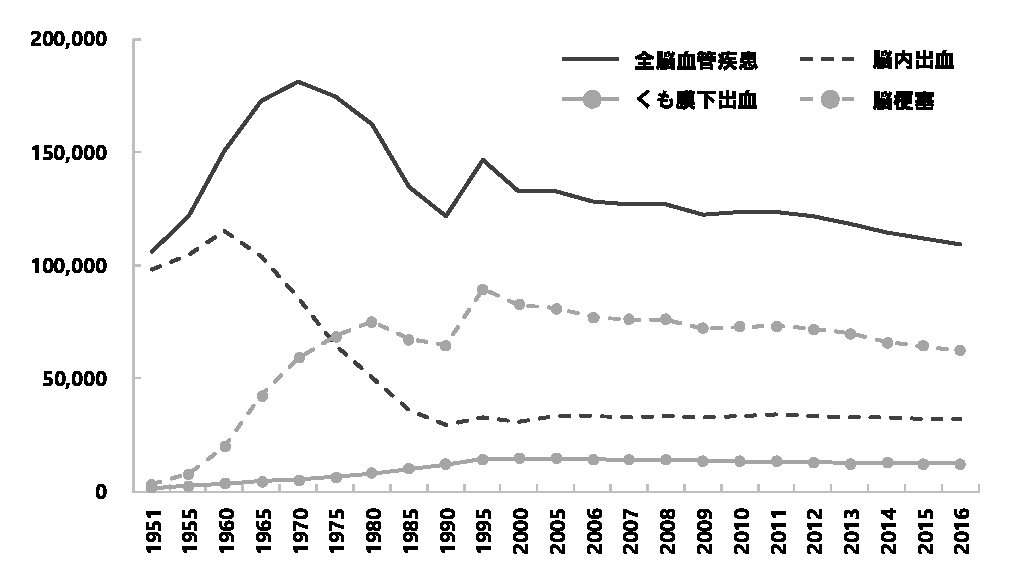
\includegraphics[width=0.95\linewidth]{./Chap1/fig/number_death.eps}
\caption{日本における脳卒中分類別死亡率の推移}
\label{fig:number_death}
\end{center}
\end{figure}

脳卒中のリハビリテーション(以下リハビリ)は,急性期,回復期,維持期の三つの区分に分けられている.
脳卒中発症直後の急性期からリハビリを行うことが勧められている\cite{脳卒中2009}.
脳卒中発症2週間後から5, 6ヶ月までの回復期において,
片側の上下肢が動かない片麻痺の患者は理学療法士から受けるリハビリを行うことで下肢の機能の再建を行う.
下肢機能の再建のための訓練により,Activities of Daily Livingの向上,Quality of Lifeの向上が見込める.
さらには維持期に長期的に運動機能を維持することで,社会復帰を図る.

%%%%%%%%%%%%%%%%%%%%%%%%%%%%%%%%%%%%%%%%%%%%%%%%%%%%%%%%%%%%%%%%%%%%%%%%%%%%%%%%%%%%%%%%%%%%%%%%%%%%%%%%%%%%%%%%%%%%%%%%%%%%%%%%%%%
\section{リハビリテーションへのロボットの介入}
\label{sec:robotics_chap1}
近年のロボット技術の向上により,リハビリの領域にロボットを介入することが期待されている.
ロボット介入の意義は
\begin{itemize}
	\item 多関節の同時コントロールが可能
	\item 正常軌道の運動が可能
	\item 負荷量の調節と負荷量の維持が可能
	\item 結果の提示,つまりフィードバックが可能
\end{itemize}
という4点である\cite{道免2015}.\\

すでに歩行運動については,歩行をアシストするロボットを用いることで歩行能力が改善された報告がある\cite{Fisher2011}\cite{Srivastava2016}\cite{有末2015}.

Fisherらは回復期の片麻痺患者に対し,理学療法士による従来のリハビリとアシストロボットを利用したトレッドミルでの歩行によるリハビリ(Robot Assisted Gait Trainig,以下RAGT)を比較した.
アシストロボット(Autoambulator)は患者を吊り下げるハーネスと,股関節・膝関節を補助する外骨格の駆動装置から成る.外観を図\ref{fig:autoambulator}に示す.
どちらの患者群でもリハビリの前後で,8 m歩行,3分歩行,Tinettiバランステストの全てにおいて優位にスコアが上昇した.
なお,理学療法士による従来のリハビリとRAGTによるリハビリとの間ではリハビリ後のスコアに差は無かった.

\begin{figure}[b]
	\begin{center}
		\includegraphics[width=4.5cm]{./Chap1/fig/Autoambulator.PNG}
		\caption{Autoambulatorによるリハビリの様子\cite{Fisher2011}}
		\label{fig:autoambulator}
	\end{center}
\end{figure}

Srivastavaらも理学療法士のリハビリとRAGTのリハビリを比較している.
麻痺側の足に外骨格(ALEX)を装着し,健常者の軌道から外れた時だけ支援する.
外観を図\ref{fig:ALEX}に示す.
Fisherらの結果と同様,どちらのリハビリでも患者の運動機能は改善したがスコアの上昇に差はなかった.
RAGTのリハビリの方が理学療法士の負担が減ると結論づけている.

\begin{figure}[b]
	\begin{center}
		\includegraphics[width=8cm]{./Chap1/fig/ALEX.PNG}
		\caption{RAGTのリハビリの様子\cite{Srivastava2016}}
		\label{fig:ALEX}
	\end{center}
\end{figure}

有末らは回復期の片麻痺患者に対し,Honda歩行アシストを用いた歩行練習を検討した.
Honda歩行アシストは股関節の屈曲・伸展運動を大腿部のフラームを通じて補助する.
装着者の歩行周期に合わせて,股関節の屈曲・伸展のタイミングを補正する\cite{渡邊2016}.
訓練前の歩行速度が60 m/min未満の患者において,歩行速度や歩行の幅が増加した.\\

本研究では回復期のリハビリにおける片麻痺患者の起立動作に着目する.
運動機能が低下すると生活範囲が狭まる\cite{Guralnik1994}ため,日常生活の中で活動の起点となる起立動作の訓練が必要である.
入院中や退院後について理学療法士がいない中でも,廃用性症候群を防ぐために起立動作を行わなければならない.
よって,自立を促すための起立動作の支援への要求があり,片麻痺患者の起立動作を支援する機器の開発が重要である.
%次項にて起立動作の支援機器に関する従来研究について述べる.

\clearpage

%%%%%%%%%%%%%%%%%%%%%%%%%%%%%%%%%%%%%%%%%%%%%%%%%%%%%%%%%%%%%%%%%%%%%%%%%%%%%%%%%%%%%%%%%%%%%%%%%%%%%%%%%%%%%%%%%%%%%%%%%%%%%%%%%%%

\section{起立動作の支援機器に関する従来研究}
\label{sec:related_research_chap1}

起立動作の支援機器に関する従来研究について述べる.
%支援機器は大きく分けて2つに分類することができる.
多くの片麻痺患者は非麻痺側の足からの感覚入力が受け取れないため,姿勢制御が不安定になる\cite{Chou2003}.
そのため,健側の足に体重を乗せて立ち上がるので動作は左右で非対称なものとなり,健側の足に大きな負担がかかってしまう.
リハビリテーションにおいては麻痺側の足をいかに活用し,左右対称な動きにするかが重要である.

起立動作の支援機器の従来研究として,起立動作を外骨格などにより支援するもの\cite{Tsukahara2010}と座面が上昇することで支援するもの\cite{Shiraishi2016}がある.

TsukaharaらはロボットスーツHALを用いて完全片麻痺患者の起立動作を支援するシステムを開発した.
腰・膝・足関節の運動を支援するHALと,前方に倒れないようにするために腰をサポートするハーネスでシステムは構成されている.外観を図\ref{fig:HAL}に示す.
システムは脛が前傾し,足部の圧力中心がある閾値を超えるかどうか判断することで使用者の動作意図を読み取り,起立動作を支援する.
完全片麻痺患者1名に対して実験を行い,安定して立ち上がることができたと報告している.

\begin{figure}[b]
	\begin{center}
		\includegraphics[width=10cm]{./Chap1/fig/HAL.PNG}
		\caption{HALを用いた支援の様子\cite{Tsukahara2010}}
		\label{fig:HAL}
	\end{center}
\end{figure}

Shiraishiらは座面が直線的に移動することで片麻痺患者の起立動作を支援するシステムを開発した.
床反力から使用者の動作意図を読み取り,座面が臀部を直線的に押し上げることで起立動作を支援する.外観を図\ref{fig:Handrail}に示す.
2名の片麻痺患者と1名の四肢麻痺患者に対して実験を行い,麻痺側と非麻痺側の足の使用率の差が減少したと報告している.

\begin{figure}[b]
	\begin{center}
		\includegraphics[width=10cm]{./Chap1/fig/Handrail.PNG}
		\caption{支援の様子\cite{Shiraishi2016}}
		\label{fig:Handrail}
	\end{center}
\end{figure}


これらの従来研究は関節に力を補助するような筋力増強が主である.
運動を最初から最後まで支援することなり,支援のしすぎとなる可能性がある.
しかし,運動を支援する際には,運動のメカニズムを理解したうえで支援することが重要である.



\clearpage
%%%%%%%%%%%%%%%%%%%%%%%%%%%%%%%%%%%%%%%%%%%%%%%%%%%%%%%%%%%%%%%%%%%%%%%%%%%%%%%%%%%%%%%%%%%%%%%%%%%%%%%%%%%%%%%%%%%%%%%%%%%%%%%%%%%
\section{研究の目的}
\label{sec:objective_chap1}

\ref{sec:background_chap1}節で,脳卒中により片麻痺となった患者のリハビリの重要性について述べた.
\ref{sec:robotics_chap1}節で,歩行動作のリハビリに投入されるロボットについて,\ref{sec:related_research_chap1}節で起立動作の支援機器について述べた.
しかし,従来の支援機器ではヒトの運動のメカニズムを理解した上で動作を支援していないことが明らかになった.\\

本研究ではヒトの運動のメカニズムを理解し,片麻痺患者のリハビリを日常的に支援する機器を開発する.
本研究の対象者は回復期の片麻痺患者であり,入院中に日常的に使用することでリハビリを行うことを目指す.
まず,片麻痺患者が理学療法士によるリハビリを受けてどのように起立動作が変化するかを調査する.
起立動作の変化をヒトの運動のメカニズムに沿って捉えることで,リハビリの効果を検証する.
次に,片麻痺患者の起立動作のリハビリにおける理学療法士の技能を解析する.
理学療法士は片麻痺患者の起立動作の最初から最後まで力を入れているわけではなく,特定のタイミングで起立動作を支援している.
特定のタイミングで支援する技能を解析することで,起立動作の支援機器に応用する.
そして,起立動作の支援機器を開発し,機器の有効性を検証する.

以上より,本研究の目的を以下のように3つ設定する.
%\begin{center}
%\doublebox{
%	\begin{tabular}{c}
		\begin{enumerate}
			\item 理学療法士の介入による片麻痺患者への影響を調査
			\item 理学療法士の技能を解析
			\item 理学療法士の技能を活用した,起立動作の支援機器の開発
		\end{enumerate}
%	\end{tabular}
%}
%\end{center}





\clearpage


%%%%%%%%%%%%%%%%%%%%%%%%%%%%%%%%%%%%%%%%%%%%%%%%%%%%%%%%%%%%%%%%%%%%%%%%%%%%%%%%%%%%%%%%%%%%%%%%%%%%%%%%%%%%%%%%%%%%%%%%%%%%%%%%%%%
\section{本論文の構成}

本論文は全6章から構成されている.本論文の構成を図\ref{fig:thesis_flow}に示す.

第1章では,本研究の背景と従来研究,目的について述べた.

第2章では,問題設定を明らかにし,本研究におけるアプローチについて述べる.

第3章では,理学療法士のリハビリテーションによる片麻痺患者への影響について述べる.

第4章では,理学療法士のリハビリテーションの技能について述べる.

第5章では,起立動作の支援機器への応用と有効性を検証するために行った実験について述べる.

第6章では,本研究の結論と今後の展望について述べる.

%\clearpage


\begin{figure}[b]
\begin{center}
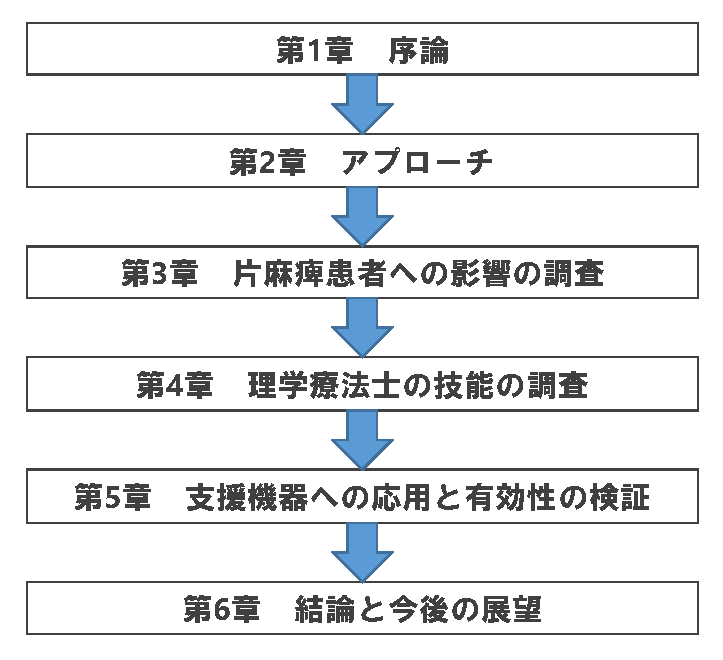
\includegraphics[width=8cm]{./Chap1/fig/thesis_flow.eps}
\caption{本論文の構成}
\label{fig:thesis_flow}
\end{center}
\end{figure}

\clearpage



%%%%%%%%%%%%%%%%%%%%%%%%%%%%%%%%%%%%%%%%%%%%%%%%%%%%%%%%%%%%%%%%%%%%%%%%%%%%%%%%%%%%%%%%%%%%%%%%%%%%%%%%%%%%%%%%%%%%%%%%%%%%%%%%%%%
%%% Local Variables:
%%% mode: katex
%%% TeX-master: "../thesis"
%%% End:

\chapter{本研究のアプローチ}
\label{chap:approach}
\minitoc

\thispagestyle{empty}

\newpage
%%%%%%%%%%%%%%%%%%%%%%%%%%%%%%%%%%%%%%%%%%%%%%%%%%%%%%%%%%%%%%%%%%%%%%%%%%%%%%%%%%%%%%%%%%%%%%%%%%%%%%%%%%%%%%%%%%%%%%%%%%%%%%%%%%%
\section{はじめに}
\label{sec:intro_chap2}

本章では,ヒトの運動のメカニズムを理解し,片麻痺患者の回復期のリハビリテーション(以下リハビリ)を日常的に支援する機器を開発するアプローチについて述べる.

%\ref{sec:problem_setteing_chap2}節にて,本研究における問題設定について述べる.

\ref{sec:approach_chap2}節にて,本手法のアプローチと解決すべき課題について述べる.
\ref{subsec:investigate_chap2}項にて,理学療法士のリハビリテーションにおける片麻痺患者への影響の調査について述べる.
\ref{subsec:analysys_chap2}項にて,理学療法士の技能を解析するアプローチについて述べる.
\ref{subsec:development_chap2}項にて,理学療法士の技能を応用する支援機器の開発のアプローチについて述べる.

\ref{sec:outro_chap2}節にて,本章のまとめを述べる.

\clearpage

%%%%%%%%%%%%%%%%%%%%%%%%%%%%%%%%%%%%%%%%%%%%%%%%%%%%%%%%%%%%%%%%%%%%%%%%%%%%%%%%%%%%%%%%%%%%%%%%%%%%%%%%%%%%%%%%%%%%%%%%%%%%%%%%%%%

%\section{問題設定}
%\label{sec:problem_setteing_chap2}
%第1章にて,が重要であることを述べた.\\
%
%また,\ref{sec:related_research_chap1}節にて,を述べた.などが例として挙げられる.\\
%
%また,同様に\ref{sec:related_research_chap1}節にて,であることを述べた.従って,本研究では利用する.\\
%
%上記を踏まえて,以下に本研究の問題設定をまとめる.
%\begin{itemize}
%\item 患者への影響を調査
%\item 技能を調査
%\item 支援機器を開発
%\end{itemize}
%
%このような問題設定の下,手法を提案する.
%
%
%\clearpage


%%%%%%%%%%%%%%%%%%%%%%%%%%%%%%%%%%%%%%%%%%%%%%%%%%%%%%%%%%%%%%%%%%%%%%%%%%%%%%%%%%%%%%%%%%%%%%%%%%%%%%%%%%%%%%%%%%%%%%%%%%%%%%%%%%%
\section{アプローチ}
\label{sec:approach_chap2}
\ref{sec:objective_chap1}節にて述べた通り,本研究の目的は理学療法士の介入による片麻痺患者への影響を調査,理学療法士の技能を解析,理学療法士の技能を活用した,起立動作の支援機器の開発の三つである.
それぞれの目的を達成するためのアプローチを次節で述べていく.\\

%\clearpage
%%%%%%%%%%%%%%%%%%%%%%%%%%%%%%%%%%%%%%%%%%%%%%%%%%%%%%%%%%%%%%%%%%%%%%%%%%%%%%%%%%%%%%%%%%%%%%%%%%%%%%%%%%%%%%%%%%%%%%%%%%%%%%%%%%%
\subsection{片麻痺患者への影響の調査}
\label{subsec:investigate_chap2}

理学療法士のリハビリテーションにより片麻痺患者にどのような影響があるのかを調査することを前述した.本項では,片麻痺患者への影響の調査方法について説明する.\\

起立動作は,年齢,関節角度,床反力,関節トルク,重心軌道,表面筋電図など多くの指標により調べられてきた.しかし,片麻痺患者に対してどの指標がより起立動作の特徴を捉えているか,有用な指標を抽出するような研究は行われていない\cite{長田2012}.

本研究では起立動作を運動学的な観点と表面筋電図から計算される筋シナジー構造から評価する.運動学的な観点の指標として,片麻痺患者の関節角度や重心(Center of Mass,以下CoM)の軌道を用いる.

起立動作のCoMについてはいくつかの報告がなされている.
\textcolor{red}{\cite{Mourey2000}と\cite{Yang2017}を引いて,高齢者や片麻痺患者は上体を深く曲げて起立することを記述}
%高齢者は筋肉量が低下しているため,起立の際には転倒の危険性が発生する.より安定した起立のために,若年者よりも上体を深く曲げることでCoMを足に近づけてから立ち上がる\cite{Mourey2000}.
%さらに,片麻痺患者になると健常な高齢者よりもCoMが足に近づいてから立ち上がることが分かっている\cite{Yang2017}.
\\

起立動作中の筋電図(Electromyogram,以下EMG)については以下のような報告がある.
\textcolor{red}{\cite{Silva2013}と\cite{Gross1998}を引いて,前脛骨筋の活動タイミングなどについて記述.}\\
%Silvaらは健常者と片麻痺患者を対象とし,ヒラメ筋と前脛骨筋のEMGを計測した\cite{Silva2013}.片麻痺患者において健常者よりも,麻痺と非麻痺の両側のヒラメ筋の活動タイミングが早く,麻痺側の前脛骨筋の活動タイミングが遅かったと報告している.
%また,Grossらは若年者と片麻痺患者を対象として前脛骨筋と大腿四頭筋のEMGを計測した\cite{Gross1998}.片麻痺患者において,健側の足の位置を変えることで前脛骨筋の大腿四頭筋の活動が増加することを報告した.

本研究ではヒトの運動のメカニズムを理解するべく,筋シナジー仮説を用いる.


\textcolor{red}{筋シナジー仮説とは何かを説明.}
\\

運動学的な指標や筋シナジー構造の詳細な算出方法や計測実験については第\ref{chap:investigation}章にて述べる.

%\clearpage
%%%%%%%%%%%%%%%%%%%%%%%%%%%%%%%%%%%%%%%%%%%%%%%%%%%%%%%%%%%%%%%%%%%%%%%%%%%%%%%%%%%%%%%%%%%%%%%%%%%%%%%%%%%%%%%%%%%%%%%%%%%%%%%%%%%
\subsection{理学療法士の技能解析}
\label{subsec:analysys_chap2}

片麻痺患者のリハビリテーション中において,理学療法士はどのような介入を行っているのかを調査することを前述した.本項では,理学療法士の技能の解析方法について説明する.\\

理学療法士の技能について,Tsusakaらは起立動作における理学療法士のスキル分析をしている\cite{Tsusaka2015}.
\textcolor{red}{スキル分析について記述.}\\

本研究では理学療法士の技能の調査方法として片麻痺患者に介入する腕の筋肉の表面筋電図を計測する.
理学療法士は図\ref{fig:view}に示すように,片麻痺患者の麻痺側の膝と骨盤後面に介入する.上肢の曲げ伸ばしをどのタイミングで行っているかを調査するため,理学療法士の腕の筋肉の表面筋電図を計測する.
\\

\begin{figure}[b]
	\begin{center}
		\includegraphics[width=8cm]{./Chap2/fig/view.eps}
		\caption{理学療法士による介入の様子}
		\label{fig:view}
	\end{center}
\end{figure}

理学療法士の技能の詳細な調査方法は第\ref{chap:analysys}章にて述べる.

%\clearpage

%%%%%%%%%%%%%%%%%%%%%%%%%%%%%%%%%%%%%%%%%%%%%%%%%%%%%%%%%%%%%%%%%%%%%%%%%%%%%%%%%%%%%%%%%%%%%%%%%%%%%%%%%%%%%%%%%%%%%%%%%%%%%%%%%%%
\subsection{起立動作の支援機器の開発}
\label{subsec:development_chap2}

本研究では理学療法士の技能を活用した,起立動作の支援機器の開発について前述した.
本項では,技能を活用した支援機器の従来研究について説明する.\\

\textcolor{red}{看護師の技能を活かした起立動作の支援システムを引く\cite{Chugo2007}.
	理学療法士のスキル活かした起立アシストロボットの開発を引く\cite{津坂2017}.
}\\



起立動作の支援機器の開発についての詳細な方法は第\ref{chap:development}章にて述べる.

\clearpage

%%%%%%%%%%%%%%%%%%%%%%%%%%%%%%%%%%%%%%%%%%%%%%%%%%%%%%%%%%%%%%%%%%%%%%%%%%%%%%%%%%%%%%%%%%%%%%%%%%%%%%%%%%%%%%%%%%%%%%%%%%%%%%%%%%%
\section{おわりに}
\label{sec:outro_chap2}

本章では,本研究のアプローチについて述べた.

%まず\ref{sec:problem_setteing_chap2}節にて,本研究において解決するべき課題について述べた.

\ref{sec:approach_chap2}節にて,本手法のアプローチと解決すべき課題について述べた.
\ref{subsec:investigate_chap2}節にて,理学療法士によるリハビリ中の片麻痺患者の起立動作の変化を調査するアプローチについて述べた.
\ref{subsec:analysys_chap2}項にて,理学療法士の技能を解析するためのアプローチについて述べた.
\ref{subsec:development_chap2}項にて,支援機器を開発するアプローチについて述べた.\\

次章では,技能解析について詳しく説明する.

\clearpage

%%%%%%%%%%%%%%%%%%%%%%%%%%%%%%%%%%%%%%%%%%%%%%%%%%%%%%%%%%%%%%%%%%%%%%%%%%%%%%%%%%%%%%%%%%%%%%%%%%%%%%%%%%%%%%%%%%%%%%%%%%%%%%%%%%%
%%% Local Variables:
%%% mode: katex
%%% TeX-master: "../thesis"
%%% End:

\chapter{����J�����ɂ��v���̂��߂̉摜����}
\label{chap:ImageProcessing}
\minitoc

\thispagestyle{empty}

\newpage
%%%%%%%%%%%%%%%%%%%%%%%%%%%%%%%%%%%%%%%%%%%%%%%%%%%%%%%%%%%%%%%%%%%%%%%%%%%%%%%%%%%%%%%%%%%%%%%%%%%%%%%%%%%%%%%%%%%%%%%%%%%%%%%%%%%
\section{�͂��߂�}
\label{sec:}

%\textcolor{red}{�{�͉͂��M�C������\��ł��D�}���ς��DOCamCalib�̎��ƃ��f���m�F}

�{�͂ł́C����J�����Ŏ擾�����摜�ɂ���ăI�[������3�����v�����s�����߂ɗp������W�n��K�v�ȃp�����[�^�C�摜�����ɂ‚��ďq�ׂ�D
%�{�����ł́C�n��̈قȂ镡���n�_�ɋ���J������ݒu���C�����������Ƃ��ăI�[�������B�e�����摜����͉摜�Ƃ���D
%���͉摜�̂���1�΂̓��͉摜��p���ăI�[�����̃X�e���I�v�����s�����C�J�����̈ʒu��p�����قȂ邽��2��̃J�����ɋ��ʂȍ��W�n��݂���D��������N�e�B�t�@�C�h���W�n�ƌĂԁD
%�ݒu���ꂽ�ʒu��p���̈قȂ�2��̃J�����摜��p���ăX�e���I�v�����s�����߁C2��̃J�����ɋ��ʂȍ��W�n��݂��C��������N�e�B�t�@�C�h���W�n�ƌĂԁD
%�{�����ł͋���摜��p�����v�����ȒP�ɂ��邽�߂ɁC�摜�����ɂ���ē��͉摜�����N�e�B�t�@�C�h���W�n�摜�֕ϊ����C����ɋ��჌���Y�ɋN������c�݂��������������e�摜�ւƕϊ�����D
%����摜�͋��჌���Y�̌��w���f���ɂ���ĕω����邽�߁C�g�p���鋛�჌���Y�̃��f���Ɋ�Â��ĉ摜�̍��W�ϊ���c�݂̏������s���D
%�܂��C�摜��ϊ�����ۂɕK�v�ȃJ�����̓����p�����[�^��O���p�����[�^�𐄒肷��D\\

�܂�\ref{sec:gaiyou2}�߂ł͖{�͂ōs���摜�����̊T�v�ɂ‚��ďq�ׂ�D

����\ref{sec:rectified}�߂Ŗ{�����ŋ���摜�΂𕽍s�X�e���I�y�A�Ƃ��Ĉ������߂ɒ�`������W�n�ɂ‚��ďq�ׂ�D

\ref{sec:fisheye_model}�߂ł́C��ʓI�ȃJ�����Ƌ���J�����̈Ⴂ�ɂ‚��ďq�ׂ���C���჌���Y�ɂ��c�݂̃��f���ɂ‚��Đ�������D�����Ė{�����ŗp���鋛��J�����̃��f���ɂ‚��ďq�ׂ�D

\ref{sec:calibration}�߂Ŗ{�����ɂ�����摜�����ɕK�v�ȃp�����[�^�ƁC�����̐�����@�ɂ‚��ďq�ׂ�D

\ref{sec:translation}�߂ł́C���͉摜�΂𕽍s�X�e���I�摜�΂ւƕϊ�����摜������@�ɂ‚��ďq�ׂ�D�摜�̕ϊ��ɂ�\ref{sec:rectified}�߂Œ�`�������W�n��\ref{sec:calibration}�߂Ő��肵���p�����[�^��p����D

%���̍��W�n�ւ̉摜�̕ϊ����@�ɂ‚��ďq�ׂ�D�ϊ��ɂ�\ref{sec:calibration}�߂Ő��肵���p�����[�^��p����D

�Ō��\ref{sec:undistortion}�߂ł́C���͉摜���狛�჌���Y�ɂ��c�݂���菜���������e�摜�ւƕϊ������@�ɂ‚��ďq�ׂ�D
%�Ō��\ref{sec:backsubtraction}�߂ł́C�����_���o�̂��߂ɉ摜������I�[�����̈�𒊏o����w�i�����ɂ‚��ďq�ׂ�D
\clearpage
%%%%%%%%%%%%%%%%%%%%%%%%%%%%%%%%%%%%%%%%%%%%%%%%%%%%%%%%%%%%%%%%%%%%%%%%%%%%%%%%%%%%%%%%%%%%%%%%%%%%%%%%%%%%%%%%%%%%%%%%%%%%%%%%%%%
\section{����J�����ɂ��v���̂��߂̉摜�����̊T�v}
\label{sec:gaiyou2}

��Ď�@�ł�2��̃J�����ŎB�e����1�΂̃I�[�����摜����Ή��_�����o���C�O�p���ʂ̌�������I�[������3�����`����v������D
���̂悤�ȃX�e���I�v���ɂ����ẮC2��̃J�����̍����𑵂����ꂼ��̌��������s�ɂȂ�悤�ɐݒu�������s�X�e���I�v���������s���Ă���D
�J�����𕽍s�X�e���I�y�A�Ƃ��邱�ƂŃG�s�|�[���􉽂ƌĂ΂��􉽏��������������m�ɗ��p�”\�ƂȂ�C
�摜�Ԃ���̑Ή��_���o�̑��x�␸�x�̌��オ���҂����D
�����Ŗ{�����ɂ����Ă��C�J�����𕽍s�X�e���I�y�A�Ƃ��v������D\\

������2��̃J�����̐ݒu�ʒu��p�x�𒲐��ł���ꍇ�C�����I�Ɍ����ɕ��s�X�e���I�y�A�ƂȂ�悤�J������ݒu���邱�Ƃ͗L���Ȏ�i�ł���D
�������I�[�����v���ɏ\���Ȏ����𓾂邽�߂ɂ́C�ݒu����J�����Ԃ̋�����傫������K�v������C
�����I�Ɍ����ȕ��s�X�e���I�y�A�Ƃ��邱�Ƃ͍���ł���ƍl������D
�����Ŗ{�����ł͉摜�����ɂ���ĉ摜�΂𕽍s�X�e���I�J�����ɂ���Ď擾�����摜�΂ɂȂ�悤�ϊ�����i\ref{sec:translation}�߁j�D
�摜�����ɂ���ĉ摜�΂𕽍s�����邽�߂ɂ́C�L�����u���[�V�����ɂ���ăJ�������L�̘c�݂�C�J�����̐ݒu�ʒu���]�Ƃ������p�����[�^�𐄒肷��K�v������i\ref{sec:calibration}�߁j�D
���̂悤�ȃp�����[�^���擾���邽�߂ɁC�܂��J���������s�ƂȂ���W�n��{�����Ŏg�p���鋛�჌���Y�ɂ��c�݂̃��f�����`����i\ref{sec:rectified}�߁C\ref{sec:fisheye_model}�߁j�D\\

�{�����ł͋���J�������g�p���邽�߁C������摜�͑傫�Șc�݂������Ă���D
��ʓI�ɋ���摜����̑Ή��_���o�́C�ʏ�̃����Y�ŎB�e�����摜�΂���̑Ή��_���o�ɔ�ד�Փx�������Ȃ�D
�����Ŗ{�����ł͑Ή��_���o�̑O�ɁC���s�������摜�΂���摜�����ɂ���ċ���摜���狛�჌���Y���L�̘c�݂���������i\ref{sec:undistortion}�߁j�D
�c�݂̏����ɂ́C�L�����u���[�V�����ɂ���Ď擾�����p�����[�^��p����D




\clearpage
%%%%%%%%%%%%%%%%%%%%%%%%%%%%%%%%%%%%%%%%%%%%%%%%%%%%%%%%%%%%%%%%%%%%%%%%%%%%%%%%%%%%%%%%%%%%%%%%%%%%%%%%%%%%%%%%%%%%%%%%%%%%%%%%%%%%
\section{���N�e�B�t�@�C�h���W�n}
\label{sec:rectified}

�{�����ł͒n��̈قȂ镡���n�_�ɋ���J������ݒu���C�S�ẴJ�����Ŏ����������Ƃ��ĎB�e�����I�[�����̉摜����͉摜�Ƃ���D
�����n�_����B�e�������͉摜�̂����C2�n�_����B�e����1�΂̓��͉摜��p���ăX�e���I�v�����s���D
�X�e���I�v���ł͈�ʓI�ɁC�����Ɛ��x�����コ���邽�߂ɃG�s�|�[���􉽂ƌĂ΂��􉽊w�I�ȍS���������p������\cite{cox1996}�D%���̃G�s�|�[���S�����摜��ŊȒP�Ɉ�����Ƃ������R����C�J�����𕽍s�ɐݒu�������s�X�e���I�v����
�{�����ł́C�G�s�|�[���S���̉摜��ł̈�����e�Ղɂ��邽�߂ɁC�J�����𕽍s�ɐݒu�������s�X�e���I�v�����s���D
�������}\ref{fig:camera_install}�̂悤�ɃI�[�����͍��x100 km�ȏ�̏��Ŕ������邽��\cite{jones1971}�C�O�p���ʂɂ��v���ɏ\���Ȏ����𓾂邽�߂�2��̃J�����͑傫�������������Đݒu����K�v������D
���̂���2��̃J�����̎p����ݒu���ɒ��߂��邱�Ƃɂ���Đ��m�ȕ��s�X�e���I�y�A�ɂ��邱�Ƃ͍���ł���D
�����ʼn摜�����ɂ����͉摜�΂𕽍s�X�e���I�摜�΂ւƕϊ�����K�v������D\\
%�������I�[�����͍��x100 km�ȏ�̏��ɔ������錻�ۂł��邽��[���p�\��]�C�X�e���I�v�����邽�߂ɂ̓J�����Ԃ̋�������ɑ傫������K�v������C�J�����𕽍s�X�e���I�y�A�ɂ��邱�Ƃ͍���ł���D�����ʼn摜�����ɂ���ē��͉摜�΂𕽍s�X�e���I�摜�΂ւƕϊ�����K�v������D\\

\begin{figure}[b]
\begin{center}
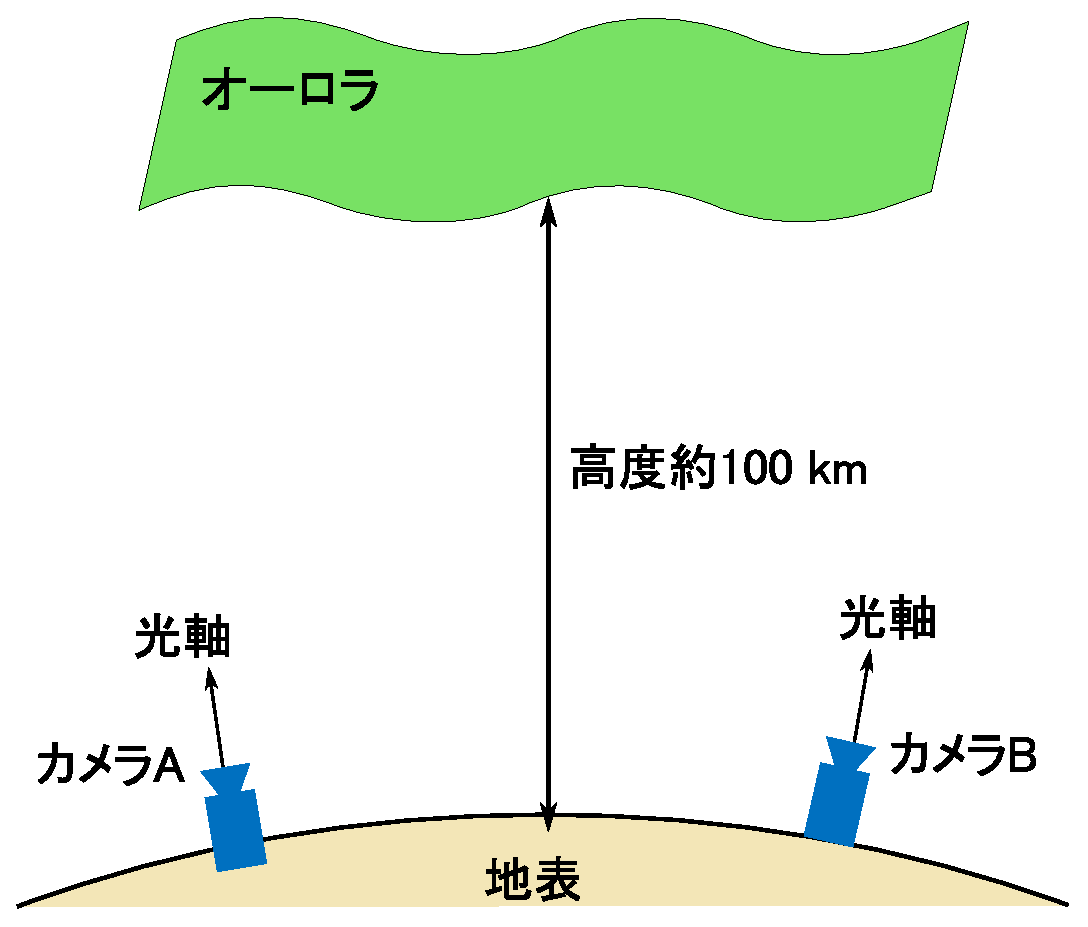
\includegraphics[width=7cm]{./chap3/eps/CameraInstall.eps}
\vspace{5mm}
\caption{�I�[�����̍��x�ƃJ�����ݒu�ʒu�̊֌W}
\label{fig:camera_install}
\end{center}
\end{figure}

���͉摜�΂𕽍s�X�e���I�摜�΂ւƕϊ����邽�߂ɁC2��̃J�����ɋ��ʂȍ��W�n��݂���D
���̍��W�n�����N�e�B�t�@�C�h���W�n�ƌĂԁD
2��̃J���������ꂼ��J����A�C�J����B�ƌĂԂ��ƂƂ���D�J����A�C�J����B�ƃ��N�e�B�t�@�C�h���W�n�Ƃ̊֌W��}\ref{fig:RicthifiedCoordinate}�Ɏ����D
���N�e�B�t�@�C�h���W�n�̌��_���J����A�̌��w���S�Ƃ��CX�����J����A�̌��w���S����J����B�̌��w���S�֌����������ƒ�`����D
X����Y���ɐ����ŁC�n�\����V�������Ɍ�����������Z�����Ƃ�D
�܂��CY���͉E��n�ɏ]���C���_�ɂ�����n�\�ʂ̐ݒu���ʂ�X���ɐ����ȕ����ƒ�`����D\\

�e�J�����̎p���ƃ��N�e�B�t�@�C�h���W�n�̊֌W��}\ref{fig:rictify_rotate}�Ɏ����D
�ݒu���ꂽ�J����A�̌�����$Z_A$�ŕ\���C$X_A$���C$Y_A$���͓�����摜�̍��W���ɕ��s�Ȏ���\���Ă���D�J����B�Ɋւ��Ă����l�ɕ\���Ă���D
�Ԃ����ŕ\�����������N�e�B�t�@�C�h���W�n�̊e����\���Ă���D
�J����A�̊e�������N�e�B�t�@�C�h���W�n�̊e���ƈ�v����悤�ȉ�]�s���$R_A$�Ƃ���D
�J����B��$X_B$�������N�e�B�t�@�C�h���W�n��$X$���ƈ�v�����C$Y_B$����$Z_B$�������N�e�B�t�@�C�h���W�n��$Y$����$Z$���ɕ��s�ƂȂ�悤�ɂ����]�s���$R_B$�Ƃ���D
�J����A�C�J����B�����ꂼ��$R_A$�C$R_B$��]������Ƃ��C2��̃J�����͕��s�X�e���I�y�A�ƂȂ�D
�܂��C�J�����ԋ�����$d$�Ƃ���ƁC���N�e�B�t�@�C�h���W�n�ɂ����ăJ����A�̍��W��$(0, 0, 0)$�C�J����B�̍��W��$(d, 0, 0)$�ƕ\�����D

%\clearpage

%\textcolor{red}{�i�}�C���\��j}



\begin{figure}[hbp]
\begin{center}
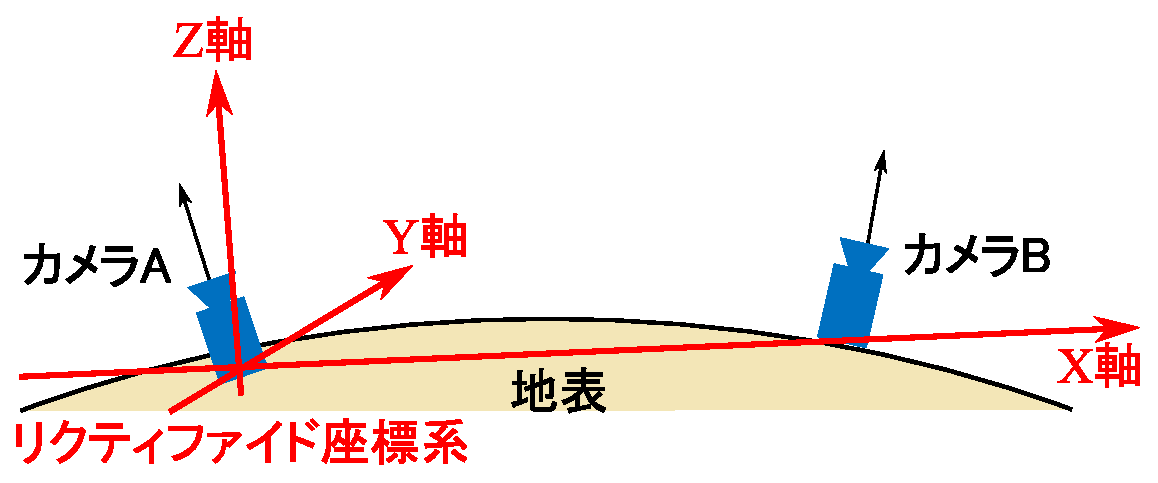
\includegraphics[width=8cm]{./chap3/eps/RicthifiedCoordinate.eps}
\vspace{5mm}
\caption{�J�����̍��W�n�ƃ��N�e�B�t�@�C�h���W�n�̊֌W}
\label{fig:RicthifiedCoordinate}
\end{center}
\end{figure}

%\subsection{���N�e�B�t�@�C�h���W�n�ւ̓��͉摜�ϊ�}
%\label{ssec:rectification}
\begin{figure}[hbp]
\begin{center}
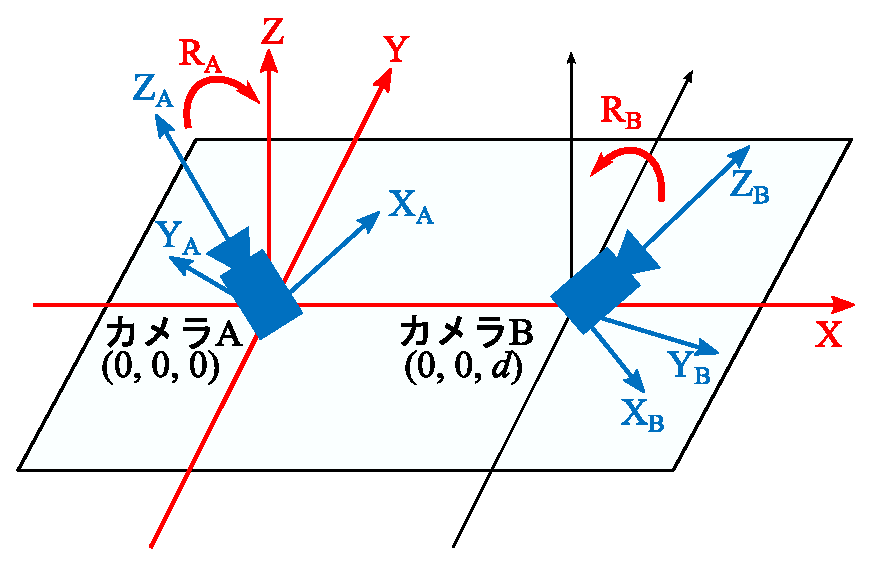
\includegraphics[width=8cm]{./chap3/eps/RecthifyRotate.eps}
\caption{���N�e�B�t�@�C�h���W�n�ւ̃J�����p���̕ϊ�}
\label{fig:rictify_rotate}
\end{center}
\end{figure}

\clearpage

%%%%%%%%%%%%%%%%%%%%%%%%%%%%%%%%%%%%%%%%%%%%%%%%%%%%%%%%%%%%%%%%%%%%%%%%%%%%%%%%%%%%%%%%%%%%%%%%%%%%%%%%%%%%%%%%%%%%%%%%%%%%%%%%%%%
\section{���჌���Y�̃��f��}
\label{sec:fisheye_model}

�摜�����ɂ���ēK�؂ɉ摜��ϊ������m�Ɍv�����s�����߂ɁC�J�����ɓ��˂�������Ƃ��ꂪ���e�����摜���W�Ƃ̊֌W�𐳂����m�邱�Ƃ͕s�Œ��ł���D
�ʏ�̃J�����̃����Y�͈�ʓI�ɓ������e�ˉe�������p�����C�J�����ւ̓��ˌ��̒P�ʃx�N�g�����i$x$, $y$, $z$�j�C�摜���S��($C_u$, $C_v$)�C�œ_������$f$�Ƃ���Ɠ��e�_�̉摜���W�i$u$, $v$�j�͈ȉ��̎�(\ref{eq:NormalCamera})�ɂĕ\�����D

\begin{equation}
\begin{bmatrix}
u\\
v
\end{bmatrix}
=
\begin{bmatrix}
f{x}/{z}\\
f{y}/{z}
\end{bmatrix}
\label{eq:NormalCamera}
\end{equation}

����C��Ď�@�ł͋��჌���Y��p����D���჌���Y�͓��ˌ��������Y�ő傫�����܂��邽�߁C���ˌ��Ɠ��e�_�Ƃ̊֌W����ʓI�ȃJ�����̎�(\ref{eq:NormalCamera})�Ƃ͈قȂ�D
�ʏ�̃����Y�Ƌ��჌���Y�ɂ����ˌ��Ɠ��e�_�Ƃ̊֌W�̈Ⴂ��}\ref{fig:lensmodel}�Ɏ����D\\

\begin{figure}[b]
  \centering
  \subfigure[�ʏ�̃����Y�̎ˉe���f��]{
    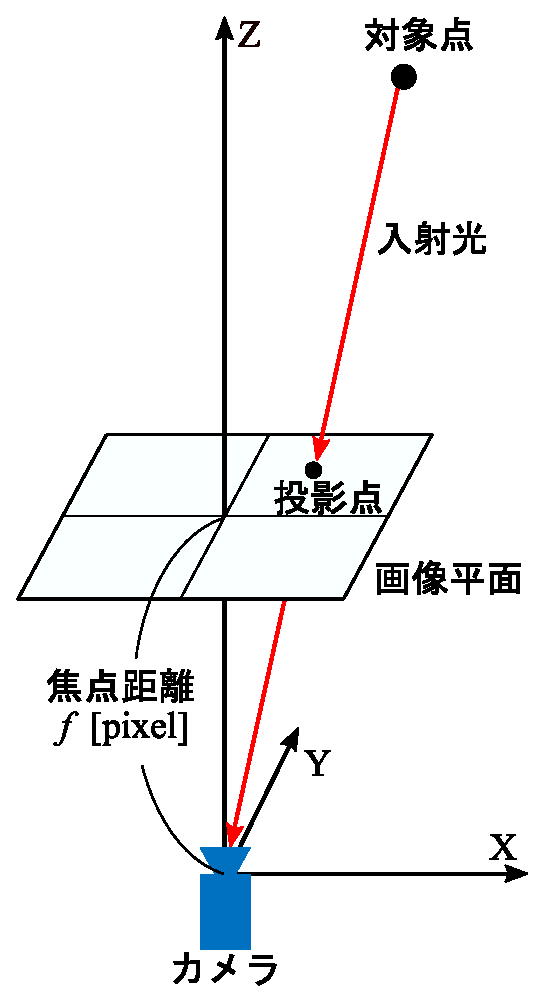
\includegraphics[width=4cm]{./chap3/eps/PerspectiveModel.eps}
  \label{fig:perspective_model}}
\hspace{2cm}
  \subfigure[���჌���Y�̎ˉe���f��]{
    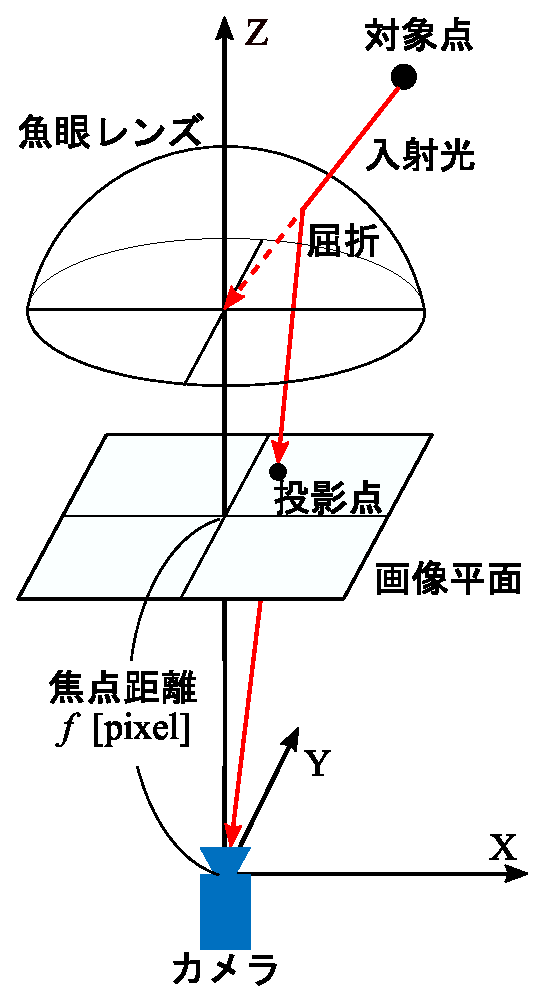
\includegraphics[width=4cm]{./chap3/eps/FisheyeModel.eps}
  \label{fig:fisheye_model}}
%\vspace{10mm}
  \caption{�ʏ�̃����Y�Ƌ��჌���Y�̎ˉe�̈Ⴂ}
  \label{fig:lensmodel}
\end{figure}

���჌���Y�Ƃ́C�L�`�ɖ�$180^{\circ}$���x�̍L����p�������������Y�̂��Ƃ��w�����C�����‚��̎�ނɕ��ނ����D
�C���[�W�T�[�N���a����ʂ̑Ίp�������傫�����჌���Y�͑Ίp���჌���Y�ƌĂ΂�C
��ʓI�ȃJ�������l�ɉ�ʑS�̂ɉf�����f��D
���΂ɃC���[�W�T�[�N������ʂ̍����C���������������჌���Y�͉~�����჌���Y�ƌĂ΂�C��p���̑S�Ẳf�����摜���̉~�`�̗̈�ɉf��D
�Ίp����摜�Ɖ~������摜�̈Ⴂ��}\ref{fig:DiagonalCircle}�Ɏ����D
�B��������p�͈قȂ邪�C�ǂ���̋�������ł����Ă�������摜�͋��჌���Y���L�̘c�݂�L���Ă���C
�c�݂̓����Y�̎ˉe�����Ɉˑ�����D\\



��L�̒ʂ苛�჌���Y�͎ˉe�����ɂ���Ă����ނ����D
�Ⴆ�΃����Y�𔼋��ʂƉ��肵���ꍇ�ɁC������̐}�`�����̂܂ܕ��ʂɎˉe���鐳�ˉe������C���ʏ�̋��������������e�����p�ɂ��𑜓x�̈Ⴂ�̂Ȃ��������ˉe�����C���̖ʐς����̊p�ɔ�Ⴗ�铙���̊p�ˉe�����Ȃǂ̎ˉe���������݂���D
���̎ˉe�����̈Ⴂ������J�����ɂ���ĎB�e���ꂽ�摜�̎��“��L�̘c�݂�ω�������D
���჌���Y�̓��ˌ��Ɠ��e�_�̊֌W��}\ref{fig:tourittai}�Ɏ����D
�摜���S$(C_u, C_v)$����̃s�N�Z��������$r$[pixel]�C�J��������������ˌ��ւ̊p�x��
$\theta$ [$rad$]�C���e�_$�iu, v�j$�Ɖ摜���S�����Ԓ�����$X$���ƂȂ��p��$\phi$ [$rad$]�Ƃ��ĕ\���Ă���D
�}\ref{fig:tourittai}����$\theta$��$r$�̊֌W���ˉe�����ɂ���ĈقȂ�C�����̓����Y�ŗL�̘c�݃p�����[�^$k$ [pixel]�ɂ���Ċ֌W�t������D
�ˉe�������̉摜���S����̃s�N�Z������$r$�ƃJ��������������ˌ��ւ̊p�x$\theta$�C�c�݃p�����[�^$k$�̊֌W��\\ref{table:distortion_parameter}�Ɏ����D\\

\begin{figure}[h]
  \centering
  \subfigure[�Ίp���჌���Y�Ŏ擾�����摜]{
    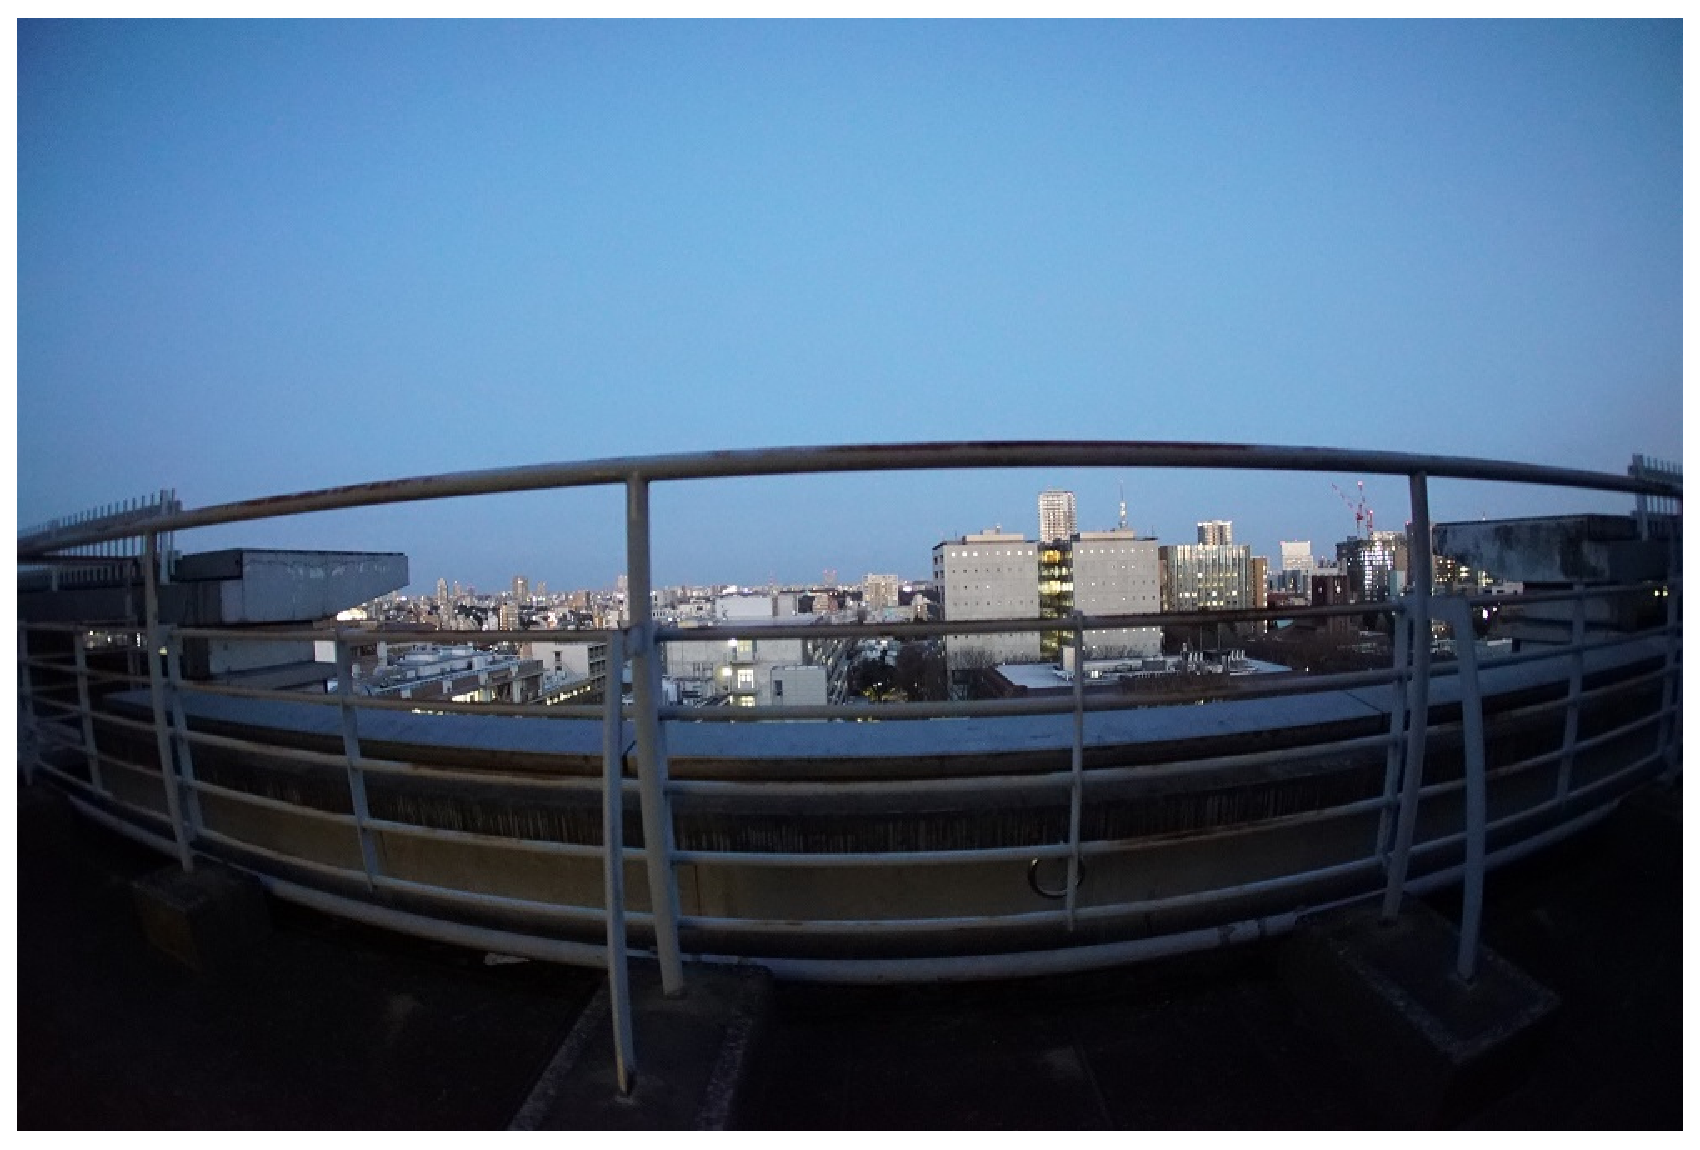
\includegraphics[width=6cm]{./chap3/eps/FisheyeDiagonal.eps}
  \label{fig:Diagonal}}
  \subfigure[�~�����჌���Y�Ŏ擾�����摜]{
    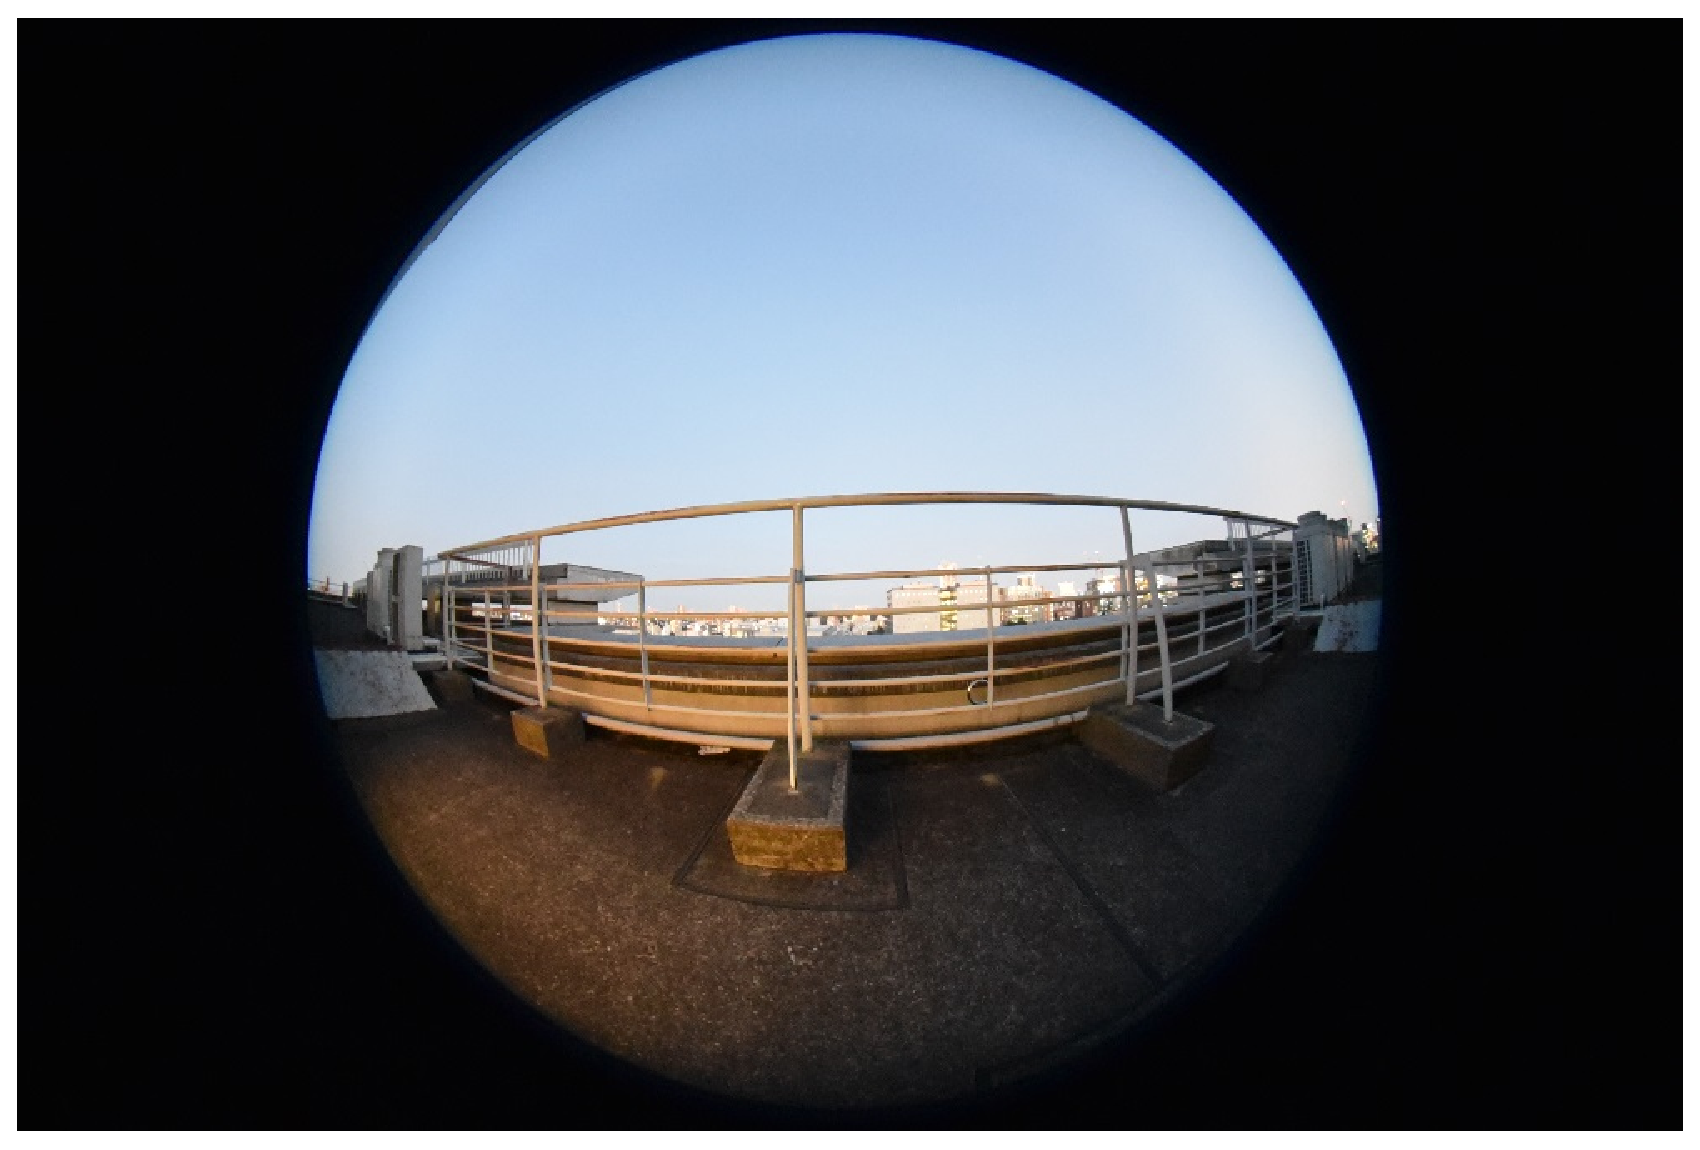
\includegraphics[width=6cm]{./chap3/eps/FisheyeCircle.eps}
  \label{fig:Circle}}
%\vspace{10mm}
  \caption{�Ίp���჌���Y�Ɖ~�����჌���Y�̈Ⴂ}
  \label{fig:DiagonalCircle}
\end{figure}

\clearpage


�}\ref{fig:tourittai}���C���e�_$�iu, v�j$�͓��ˌ��̒P�ʃx�N�g��$�ix, y, z�j$��p���Ĉȉ��̎�(\ref{eq:fisheye_uv})�C��(\ref{eq:fisheye_phi})�ŕ\�����D
�܂��C��(\ref{eq:fisheye_uv})����$r$�͕\\ref{table:distortion_parameter}�����ˌ��ƌ����Ƃ̊p�x$\theta$�Ƙc�݃p�����[�^$k$�ɂ���ĎZ�o�����D
����ăJ�����ŗL�̘c�݃p�����[�^$k$�𐄒肷�邱�Ƃŋ���摜��̃s�N�Z���Ɠ��ˌ��̕����x�N�g������ӂɊ֘A�t���邱�Ƃ��”\�ł���D\\

\begin{figure}[tb]
  \centering
  \subfigure[���ˌ��̓��e�̗l�q]{
    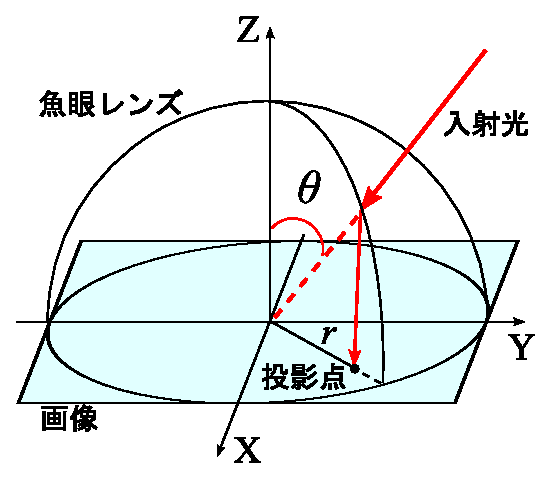
\includegraphics[width=6cm]{./chap3/eps/nyusya.eps}
  \label{fig:nyuusyakou}}
  \subfigure[���e�_$(u, v)$�ƃs�N�Z������$r$�̊֌W]{
    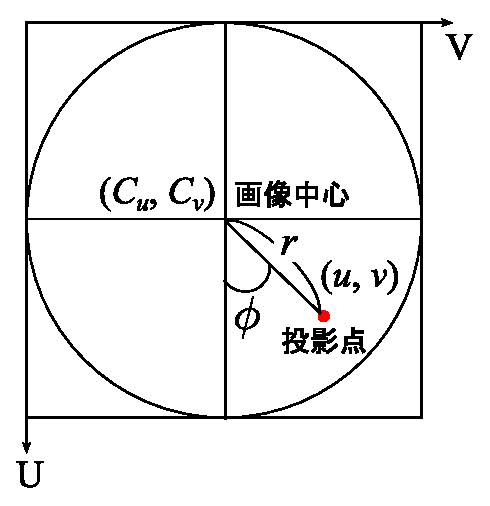
\includegraphics[width=5cm]{./chap3/eps/r2cucv.eps}
  \label{fig:pixel_kankei}}
%\vspace{10mm}
  \caption{���჌���Y�̓��ˌ��Ɠ��e�_�̊֌W}
  \label{fig:tourittai}
\end{figure}

\begin{table}[tb]
\begin{center}
\caption{�ˉe�������̉摜���S����̃s�N�Z������$r$�Ƙc�݃p�����[�^$k$�̊֌W}
\label{table:distortion_parameter}
\begin{tabular}{l c}\hline
�ˉe���� & $r$��$\theta$�̊֌W\\ \hline \hline
���ˉe���� & $r=k\sin{\theta}$ \\ 
�������ˉe���� & $r=k{\theta}$ \\
�����̊p�ˉe���� & $r=2k\sin{\frac{\theta}{2}}$ \\ \hline
\end{tabular}
\end{center}
\end{table}

\begin{equation}
\begin{bmatrix}
u\\
v
\end{bmatrix}
=
\begin{bmatrix}
r\cos\phi + C_u \\
r\sin\phi + C_v
\end{bmatrix} .
\label{eq:fisheye_uv}
\end{equation}

\begin{equation}
\phi = \cos^{-1}{\frac{x}{\sqrt{x^2 + y^2}}} = \sin^{-1}{\frac{y}{\sqrt{x^2 + y^2}}} .
\label{eq:fisheye_phi}
\end{equation}

\clearpage

���������ۂɂ̓����Y�쐬���ɐ������c�ݓ��̌�������C
�����Y�S�̂ɂ����ĕ\\ref{table:distortion_parameter}�̂悤��
�ˉe�������猈�肳���֌W���𖞂����Ă���킯�ł͂Ȃ��C�����Y���ɂ���Ă��قȂ�D
%�ɂ���đS�Ẵs�N�Z���Ɠ��ˌ��̊֌W�������ɕ\����킯�ł͂Ȃ��D
���̂��ߋ���摜�������Ɉ��������ꍇ�C�摜��̃s�N�Z���Ɠ��ˌ��̊֌W���������Y���ɎZ�o����K�v������D
�{�����ł́CScaramuzza��̎�@\cite{scaramuzza2006}�Ɠ��l�ɁC�摜���S����̃s�N�Z��������$r$�ł���s�N�Z��$(u, v)$�ƁC���ˌ��̃x�N�g��$(x, y, z)$�̊֌W����(\ref{eq:ocamcalib1})�C��(\ref{eq:uvr})�C��(\ref{eq:ocamcalib_k})�C��(\ref{eq:ocamcalib_g})�ŕ\���D
�܂����̊֌W���ɂ����āC$a_{i}$ $(i = 0,  1, 2, 3, 4)$��c�݃p�����[�^�C$r$�̊֐�$g(r)$��c�݊֐��ƌĂԂ��ƂƂ���D�L�����u���[�V�����ɂ���Ă��̘c�݃p�����[�^$a_{i}$ $(i = 0,  1, 2, 3, 4)$�����߂�D






%�����̊p�ˉe�����̑S�����჌���Y�̖͎��}��}\ref{fig:tourittai}�Ɏ����D
%�}\ref{fig:tourittai}����x���Cz���̓J�������W�n�̍��W���CU���CV���͓�����摜�̍��W����\���Ă���D
%�}\ref{fig:nyuusyakou}�͓��ˊp$\theta$�œ��˂������������Y�ŋ��܂��C�B���f�q�֓��e�����l�q��\���Ă���D�}\ref{fig:pixel_kankei}�͎B�e���ꂽ�摜��ł̉摜���S�ƁC���ړ_$(u, v)$�C�s�N�Z������$r$�̊֌W��\���Ă���D
%�\\ref{table:distortion_parameter}�Ɛ}\ref{fig:tourittai}���番����Ƃ���C�c�݃p�����[�^��m�邱�Ƃŋ���摜��̃s�N�Z���Ɠ��ˌ��̕����x�N�g�����Z�o���邱�Ƃ��”\�ł���D


\begin{equation}
\begin{bmatrix}
u-C_u\\
v-C_v\\
g(r)
\end{bmatrix}
=-k
\begin{bmatrix}
x\\
y\\
z
\end{bmatrix} .
\label{eq:ocamcalib1}
\end{equation}

\begin{equation}
r = \sqrt{(u-C_u)^2 + (v-C_v)^2} .
\label{eq:uvr}
\end{equation}

\begin{equation}
k = \sqrt{r^2 + \{g(r)\}^2} .
\label{eq:ocamcalib_k}
\end{equation}

\begin{equation}
g(r)=a_{0} + a_{1}r + a_{2}r^{2}+ a_{3}r^{3}+ a_{4}r^{4}\\
\label{eq:ocamcalib_g}
\end{equation}



\clearpage
%%%%%%%%%%%%%%%%%%%%%%%%%%%%%%%%%%%%%%%%%%%%%%%%%%%%%%%%%%%%%%%%%%%%%%%%%%%%%%%%%%%%%%%%%%%%%%%%%%%%%%%%%%%%%%%%%%%%%%%%%%%%%%%%%%%
\section{�J�����L�����u���[�V����}
\label{sec:calibration}
�O�q�̂Ƃ���C����J������ʂ��ĎB�e�����摜�̓����Y�ɂ��c�݂������Ă���D���̘c�݂�␳���邽�߂Ƀ����Y�ŗL�̃p�����[�^�𐄒肷��K�v������D
%�܂��C\ref{sec:rectified_coordinate}�߂ŏڂ����q�ׂ邪�C�{�����ł̓X�e���I�v�����s�����߂�2��̃J�����ŋ��ʂ������W�n��ݒ肷��D
�܂��C�e�J�����Ŏ擾�����摜�΂𕽍s�X�e���I�摜�΂ւƕϊ����邽�߂ɁC�n��ɐݒu���ꂽ�J�����Ԃ̈ʒu��p���𐄒肷��K�v������D
�����ŁC�{�߂ł́C�����Y�ŗL�̓����p�����[�^�ł���
�摜���S����јc�݃p�����[�^�̐����@��\ref{sec:internal_parameter}���C�O���p�����[�^�ł���J�����̈ʒu�p�����[�^��p���̉�]�p�����[�^�̐����@��\ref{sec:external_parameter}���ɂďq�ׂ�D

%\vspace{1cm}

%\begin{figure}[hbp]
%\begin{center}
%\includegraphics[width=10cm]{./chap3/tmp/parameter.eps}
%\caption{���肷��p�����[�^}
%\label{fig:parameter}
%\end{center}
%\end{figure}

%\clearpage
%\clearpage
%%%%%%%%%%%%%%%%%%%%%%%%%%%%%%%%%%%%%%%%%%%%%%%%
\subsection{�����p�����[�^�̐���}
\label{sec:internal_parameter}

�{�����ɂ����ĕK�v�ƂȂ鋛��J�����̓����p�����[�^�́C
\begin{itemize}
\item �摜���S�F$C_u$�C$C_v$
\item ���჌���Y�̘c�݃p�����[�^�F$a_{i}$ $(i = 0, 1, 2, 3, 4)$
\end{itemize}
�ł���D�Ȃ��摜���S�Ƃ̓����Y���S���猋���ʂւ̐����ƌ����ʂƂ̌�_���w���D\\%�����̐����@���ȉ��ŏq�ׂ�D
%\clearpage

%%%%%%%%%%%%%%%%%%%%%%%%%%%%%%%
%\subsubsection{�摜���S�̐���}



�{�����ł́C�����̓����p�����[�^�̐����Scaramuzza��̎�@���g�p����\cite{scaramuzza2006}�D
%����͈ȉ��̎菇�ōs���D
%�i�ȒP�Ɏ菇�������j
�B�e���u��ݒu�C�Œ肵����C�}\ref{fig:Ocam}�Ɏ����悤�Ɋi�q�p�^�[�����B�e�”\�͈͓��ňړ������Ȃ���l�X�Ȍ����p�x�ŎB�e����D�擾�����������̉摜����͉摜�Ƃ��C����J�����Ŏ擾�����摜�̉摜���S�̍��W($C_u$, $C_v$)�ƁC
�s�N�Z�����W�Ɠ��ˌ��̕����x�N�g���Ƃ��֌W�Â���c�݃p�����[�^$a_{i}$ $(i = 0, 1, 2, 3, 4)$�𐄒肷��D�{�����ɂ����Ă�10�����x�̎ʐ^����͂Ƃ����D

\vspace{1cm}

\begin{figure}[hbp]
\begin{center}
\includegraphics[width=11cm]{./chap3/tmp/ocamcalib.eps}
\caption{�����p�����[�^�̐���Ɏg�p������͉摜�̗�}
\label{fig:Ocam}
\end{center}
\end{figure}

%%%%%%%%%%%%%%%%%%%%%%%%%%%%%%%

%%%%%%%%%%%%%%%%%%%%%%%%%%%%%%%



%%%%%%%%%%%%%%%%%%%%%%%%%%%%%%%


\clearpage
%%%%%%%%%%%%%%%%%%%%%%%%%%%%%%%%%%%%%%%%%%%%%%%%%%%%%%%%%%%%%%%%%%%%%%%%%%%%%%%%%%%%%%%%%%%%%%%%%%%%%%%%%%%%%%%%%%%%%%%%%%%%%%%%%%%%%%%%%%%%%%%%%%%%%%%%%%
\subsection{�O���p�����[�^�̐���}
\label{subsec:external_parameter}

�{�����ɂ����ĕK�v�ƂȂ鋛��J�����̊O���p�����[�^�́C
\begin{itemize}
\item �J�����Ԃ̑��ΓI�Ȉʒu�p�����[�^�F�J�����ԋ���$d$�C���ʊp$\alpha$�C�Šp$\beta$
\item ��]�p�����[�^�F$\mathbf{R}$
\end{itemize}
�ł���D�����ŎZ�o�����]�p�����[�^�͊e�J�����̍��W�n�𕽍s���摜�֕ϊ����邽�߂̉�]�p�����[�^���w���D
�����̐����@���ȉ��ŏq�ׂ�D

%%%%%%%%%%%%%%%%%%%%%%%%%%%%%%%
\subsubsection{�ʒu�p�����[�^�̐���}
\label{ssec:position}
�{�����ł́C�g�p����B�e���u��GPS���j�b�g�𓋍ڂ���D����ɂ��C�B�e���u��ݒu�����ꏊ�̈ܓx�C�o�x�C�ȉ~�̍��Ƃ�����GPS�����擾���邱�Ƃ��”\�ł���D
GPS���j�b�g�ɂ���ē���e�J�����̈ʒu���𗘗p���C���N�e�B�t�@�C�h���W�n�ɂ�����J�����ԋ���$d$�𐄒肷��D
�܂�\ref{ssec:rotation}�ŏڍׂɏq�ׂ邪�C�e�J�����Ŏ擾�����摜�𕽍s���摜�ւƕϊ����邽�߂ɁC����̃J�������瑼���̃J�����ւ̕��ʊp$\alpha$�ƋŠp$\beta$���K�v�ł���D�������ʒu�p�����[�^�𗘗p���Đ��肷��D\\

�J�����ɓ��ڂ���GPS���j�b�g�ɂ��擾�����J�����ݒu�ʒu�̈ܓx��$lat$ [rad]�C�o�x��$lng$ [rad]�C�ȉ~�̍���$h$ [m]�Ƃ���D
�ȉ~�̍��Ƃ͒n����ȉ~�̂Ƌߎ������Ƃ��̑ȉ~�̂���̍����ł���D
�܂�GPS�ɂ���ē�������i$lat, lng, h$�j��p���ăJ�����ݒu�n�_�̍��W��ECEF�iEarth centered, earth fixed�j���W�n�ƌĂ΂����W�n�ŕ\������D
ECEF���W�n�͌��_��n���d�S�Ƃ��C$\rm Z^{ecef}$����n���̎��]���̖k�ɕ����C
$\rm X^{ecef}$����$\rm Z^{ecef}$���ɐ����Ŗ{���q�ߐ��̕����C$\rm Y^{ecef}$�����E��n�ł����̎��ƒ�������悤�ɒ�`�������W�n�ł���D
GPS����ECEF���W�n�Ƃ̊֌W��}\ref{fig:gps_ecef}�Ɏ����D
�܂��CGPS���$�ilat, lng, h�j$��ECEF���W�i$x^{ecef}, y^{ecef}, z^{ecef}$�j�ւƕϊ����邽�߂ɂ́C�n���̐ԓ����ϔ��a�ƝG�����Ƃ������萔���K�v�ł���D
�n���̌`���WGS84�����ȉ~�̂ƌĂ΂���]�ȉ~�̂Ƃ��ċߎ������Ƃ��C�ԓ����ϔ��a�ƝG�����͕\\ref{table:wgs84parameter}�̂悤�ɒ�߂��Ă���D\\

\begin{table}[b]
\begin{center}
\caption{WGS84�����ȉ~�̂̒萔}
\label{table:wgs84parameter}
\begin{tabular}{l c c}\hline
�p�����[�^ & �{�_�����ł̋L�� & �萔\\ \hline \hline
�ԓ��ʕ��ϔ��a �im�j & $a$ &6 378 137 \\ 
�G���� & $flat$ &1/298.257 223 563 \\ \hline
\end{tabular}
\end{center}
\end{table}

�\\ref{table:wgs84parameter}���g�p����ƁCWGS84�����ȉ~�̂̒Z���a$b$�Ɨ��S��$e$�͈ȉ��̎�(\ref{eq:WGS_b})�C��(\ref{eq:WGS_e})�ŕ\�����Ƃ��ł���D

\begin{equation}
b = a(1-flat)\\
\label{eq:WGS_b}
\end{equation}

\begin{equation}
e=\frac{\sqrt{a^2-b^2}}{a}\\
\label{eq:WGS_e}
\end{equation}


\begin{figure}[tp]
\begin{center}
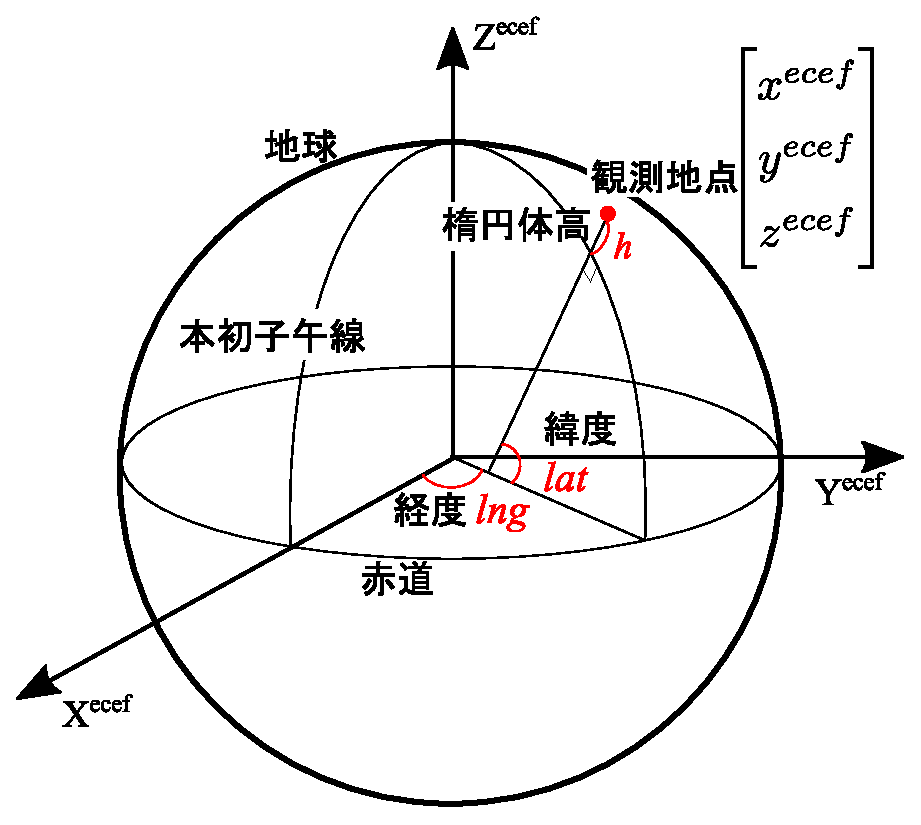
\includegraphics[width=8cm]{./chap3/eps/WGS84.eps}
\caption{GPS����ECEF���W�̊֌W}
\label{fig:gps_ecef}
\end{center}
\end{figure}

�\\ref{table:wgs84parameter}���̒萔�Ǝ�(\ref{eq:WGS_b})�C��(\ref{eq:WGS_e})��p���āC�ȉ��̎��ɂ����
GPS���$�ilat, lng, h�j$����ECEF���W$�ix^{ecef}, y^{ecef}, z^{ecef}�j$�ւƕϊ�����D\\


\begin{equation}
\begin{bmatrix}
x^{ecef}\\
y^{ecef}\\
z^{ecef}
\end{bmatrix}
=
\begin{bmatrix}
(N+h)\cos(lat)\cos(lng)\\
(N+h)\cos(lat)\sin(lng)\\
\{N(1-e^2)+h\}\sin(lat)
\end{bmatrix} .
\label{eq:GPS2ECEF}
\end{equation}

\begin{equation}
N = \frac{a}{\sqrt{1-e^2\sin^2(lat)}} .
\label{eq:WGS_N}
\end{equation}

\begin{figure}[tp]
\begin{center}
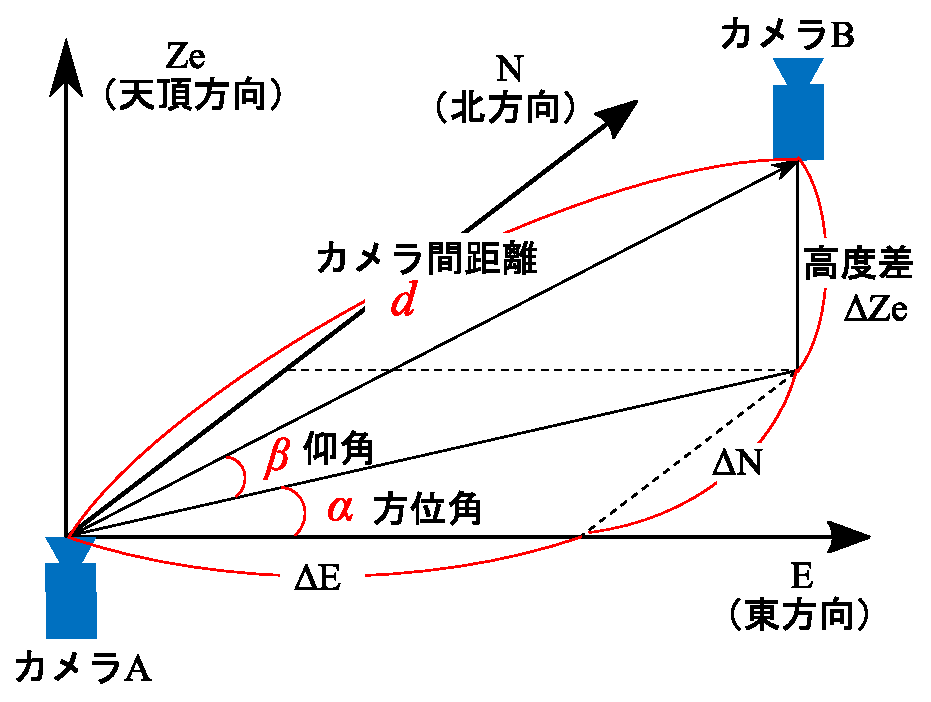
\includegraphics[width=8cm]{./chap3/eps/ENU.eps}
\caption{�J�����ԋ���$d$�C���ʊp$\alpha$�C�Šp$\beta$�̐���}
\label{fig:enu}
\end{center}
\end{figure}


���ɃJ����A�C�J����B��ECEF���W��p���āC�J�����ԋ���$d$�ƃJ��������J����B�ւ̕��ʊp$\alpha$�C�Šp$\beta$���Z�o����D
2��̃J������10 km�O��̈ʒu�ɐݒu����Ă��邽�߁C�n�\�𕽖ʂƋߎ�����D
�J����A�̐ݒu�ʒu�����_�Ƃ��C��������E���C�k������N���C�V��������Ze�����Ƃ���W�n��ݒ肷��D
���̂Ƃ��J����B��ENZe���W��$(\Delta E, \Delta N, \Delta Ze)$�Ƃ���ƁCENZe���W�n�Ƌ��߂�ʒu�p�����[�^$(d, \alpha, \beta)$�̊֌W�͐}\ref{fig:enu}�̂悤�ɂȂ�D
�܂��CENZe���W�n��ECEF���W�n��$\rm Z^{ecef}$���܂���$lng$ [rad]��]�������̂��C$\rm Y^{ecef}$���܂���$�i\pi / 2 - lat�j$ [rad]��]�����C�Ă�$\rm Z^{ecef}$���܂���$\pi / 2$ [rad]��]���������W�n�ł���D
�����ŁC�E����W�n��X���܂��CY���܂��CZ���܂���$\theta$ [rad]��]�������Ƃ��̍��W�ϊ��̍s������ꂼ��ȉ��̎�(\ref{eq:Rx})�C��(\ref{eq:Ry})�C��(\ref{eq:Rz})�̂悤�ɕ\���ƁC
$(\Delta E, \Delta N, \Delta Ze)$�͎�(\ref{eq:deltaEND})�ŎZ�o�����D



\begin{equation}
\mathbf{R}(X, \theta) =
\begin{pmatrix}
1 &0 &0 \\
0 &\cos(\theta) &\sin(\theta) \\
0 &-\sin(\theta) &\cos(\theta)
\end{pmatrix} .
\label{eq:Rx}
\end{equation}

\begin{equation}
\mathbf{R}(Y, \theta) =
\begin{pmatrix}
\cos(\theta) &0 &-\sin(\theta) \\
0 &1 &0 \\
\sin(\theta) &0 &\cos(\theta)
\end{pmatrix} .
\label{eq:Ry}
\end{equation}

\begin{equation}
\mathbf{R}(Z, \theta) =
\begin{pmatrix}
\cos(\theta) &\sin(\theta) &0 \\
-\sin(\theta) &\cos(\theta) &0 \\
0 &0 &1
\end{pmatrix} .
\label{eq:Rz}
\end{equation}

\begin{equation}
\begin{bmatrix}
\Delta E\\
\Delta N\\
\Delta Ze
\end{bmatrix}
=\mathbf{R}(Z^{ecef}, \pi /2)\mathbf{R}(Y^{ecef}, \pi /2-lat)\mathbf{R}(Z^{ecef}, lng)
\begin{bmatrix}
x^{ecef}_B - x^{ecef}_A \\
y^{ecef}_B - y^{ecef}_A \\
z^{ecef}_B - z^{ecef}_A 
\end{bmatrix} .
\label{eq:deltaEND}
\end{equation}


�}\ref{fig:enu}����C$(d, \alpha, \beta)$�͈ȏ�̎���p����$(\Delta E, \Delta N, \Delta Ze)$��p���Ď�(\ref{eq:abh})�ɂ���ĎZ�o�����D
�ȏ�̌v�Z�ɂ��C�J�����ɓ��ڂ���GPS�̏�񂩂�ʒu�p�����[�^���Z�o����D

\begin{equation}
\begin{bmatrix}
d\\
\alpha \\
\beta
\end{bmatrix}
=
\begin{bmatrix}
\sqrt{{\Delta E}^2 + {\Delta N}^2 + {\Delta Ze}^2} \\
\tan^{-1}({\Delta N}/{\Delta E}) \\
\tan^{-1}({\Delta Ze}/{\sqrt{{\Delta E}^2 + {\Delta N}^2}}) 
\end{bmatrix} .
\label{eq:abh}
\end{equation}







%%%%%%%%%%%%%%%%%%%%%%%%%%%%%%%

%\clearpage
%%%%%%%%%%%%%%%%%%%%%%%%%%%%%%%
\vspace{1cm}
\subsubsection{�J�����p�����킹�̂��߂̉�]�p�����[�^����}
\label{ssec:rotation}
%%%%%%%%%%%%%%%%%%%%%%%%%%%%%%%
\ref{ssec:position}�ڂɂĊe�J�����̈ʒu�p�����[�^�̎擾�ɂ‚��ďq�ׂ����CGPS���j�b�g���瓾������ł͊e�ʒu�ɂ�����J�����̎p�������ʂ��邱�Ƃ͂ł��Ȃ��D
�J�����̎p�������ʂ����N�e�B�t�@�C�h���W�n�ɂĊe�J�����𕽍s�X�e���I�̊֌W�ɕϊ����邽�߁C�ȉ��̎�@�ɂ���]�p�����[�^�𐄒肷��D
�{�����ł́C���̈ʒu�𗘗p���邱�Ƃʼn�]�p�����[�^�𐄒肷��D
�B�e�����摜���Ŗ��m�Ɋm�F�ł���N�‚̍P�����蓮�Ŏw�肵�C�摜���̐��ւ̕����x�N�g���ƁC���N�e�B�t�@�C�h���W�n�ɂ����鐯�ւ̕����x�N�g�����r���邱�Ƃɂ���Đ��肷��D\\
%�{�����ł͉摜���Ŗ��m�Ɋm�F�ł���N�‚̍P�����蓮�Ŏw�肷��D



�摜���擾�����ۂ̃J�������W�n�ɂ�����C�ϑ��n�_����${\it N}$�‚̊e���Ɍ����������̒P�ʃx�N�g�������ꂼ��$\mathbf{n_1}$�C$\mathbf{n_2}$...$\mathbf{n_{\it i}}$�Ƃ��C
���N�e�B�t�@�C�h���W�n�ł̊ϑ��n�_����${\it N}$�‚̊e���֌����������̒P�ʃx�N�g�������ꂼ��$\mathbf{m_1}$�C$\mathbf{m_2}$...$\mathbf{m_{\it i}}$�Ƃ���i������$i = 1, 2, ..., N$�j�D
%$(x_1, y_1, z_1)$�C$(x_2, y_2, z_2)$...$(x_i, y_i, z_i)$�i������$i = 1, 2, ..., N$�j�Ƃ���D
%�܂��C���N�e�B�t�@�C�h���W�n�ł̊ϑ��n�_����N�‚̊e���֌����������̒P�ʃx�N�g�������ꂼ��$(X_1, Y_1, Z_1)$�C$(X_2, Y_2, Z_2)$...$(X_i, Y_i, Z_i)$�i������$i = 1, 2, ..., N$�j�Ƃ���D
�܂��C$\mathbf{n_{\it i}} = (x_i, y_i, z_i)^T$�C$\mathbf{m_{\it i}} = (X_i, Y_i, Z_i)^T$�ƕ\���D
�J�����p���Ɛ��̕����x�N�g����\�����}��}\ref{fig:vector_direction}�Ɏ����D
�}\ref{fig:vector_direction}�ɂ�����ԐF�̃J�����p�������ۂ̃J�����p���C�F�̃J�����p�������N�e�B�t�@�C�h���W�n�ł̃J�����p���Ƃ���D
�_���̖��Ŏ����ꂽ���������ꂼ��̎p���ł̌��������ł���D�����Ń��N�e�B�t�@�C�h���W�n����J�������W�n�ւ̉�]�s���$\mathbf{R}$�Ƃ���ƁC
��(\ref{eq:nRm})�����藧�D
\begin{eqnarray}
\mathbf{n_{\it i}}=\mathbf{Rm_{\it i}}
\label{eq:nRm}
\end{eqnarray}

��(\ref{eq:nRm})���C�x�N�g��$\mathbf{n_{\it i}}�C\mathbf{m_{\it i}}$�����߂�Ή�]�p�����[�^�𐄒肷�邱�Ƃ��ł���D

\clearpage

%\vspace{1cm}
\begin{figure}[tb]
\begin{center}
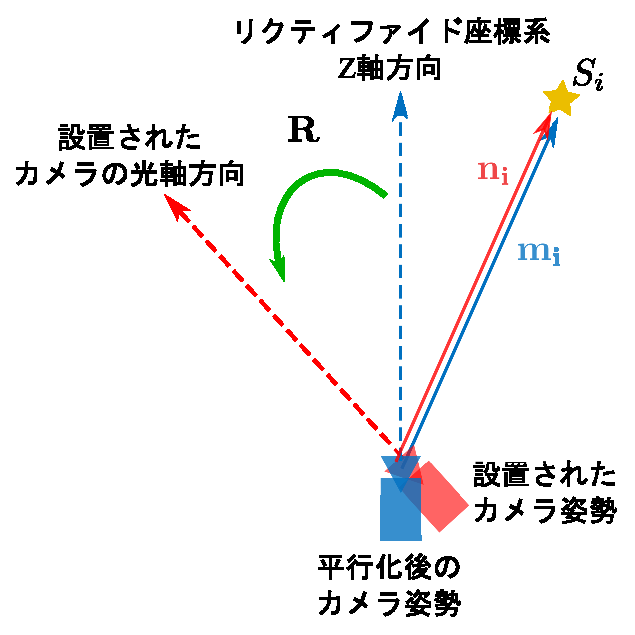
\includegraphics[width=7cm]{./chap3/eps/Camera2star.eps}
\caption{�J�����p���Ɛ��ւ̕����x�N�g��}
\label{fig:vector_direction}
\end{center}
\end{figure}


%\clearpage
%%%%%%%%%%%%%%%%%%%%%%%%%%%%%%
�ϑ��n�_����{\it i}�Ԗڂ̐�$S_i$�֌����������x�N�g��$\mathbf{n_{\it i}}$�͎�(\ref{eq:ocamcalib1})�C��(\ref{eq:ocamcalib_k})���Z�o�”\�ł���D
$S_i$�̉摜���ł̈ʒu��$(u_i, v_i)$�C�摜���S����̉摜���$S_i$�܂ł̋�����$r_i$�C�g�p���郌���Y�̘c�݊֐���$g(r)$�Ƃ���ƁC
$\mathbf{n_{\it i}}$�͎�(\ref{eq:ni})�ɂ���ċ��߂���D

\begin{eqnarray}
\mathbf{n_{\it i}}=
\left[\begin{array}{cc}x_i \\ y_i \\ z_i \end{array}\right]={\frac{1}{\sqrt{r_i^2 + g(r_i)^2}}}\left[\begin{array}{cc}u_i-C_u \\ v_i-C_v \\ g(r_i)  \end{array}\right]
\label{eq:ni}
\end{eqnarray}

�Ȃ��C�c�݊֐�$g(r)$���̘c�݃p�����[�^$a_{i}$ $(i = 0, 1, 2, 3, 4)$��\ref{sec:internal_parameter}���ŏq�ׂ��Ƃ���Scaramuzza��̎�@�ɂ��擾�”\�ł���D\\

\clearpage
%%%%%%%%%%%%%%%%%%%%%%%%%%%%%%


���Ƀ��N�e�B�t�@�C�h���W�n�ɂ�����$S_i$�ւ̕����̒P�ʃx�N�g��$\mathbf{m}_i$�����߂�D
���̂��߂ɂ́C�B�e���������ɂ�����$S_i$�̈ʒu��m��K�v�����邪�C
�C�ӂ̎����C�ʒu�C�����Ŋϑ������Ƃ��̑S�Ă̐��̈ʒu�͌����ɒm�邱�Ƃ��ł���D�܂��C���̈ʒu���v���l�^���E���`���ŕ\�����C�e�Ղɒm�邱�Ƃ��ł���悤�ɂ����\�t�g�E�F�A���������݂���D
�{�����ł́C���̒���1�‚ł���Toxsoft�Ђ��J������Stella Theater Lite���g�p����D�{�����ɂĎg�p���鐯�̒n�}�iStella Theater Lite�j��}\ref{fig:star_map}�Ɏ����D\\

\vspace{1cm}
\begin{figure}[hb]
\begin{center}
\includegraphics[width=9cm]{./chap3/tmp/StellaTheaterLite2.eps}
\caption{���̒n�}�iStella Theater Lite�j}
\label{fig:star_map}
\end{center}
\end{figure}

\clearpage

���̒n�}�֓��͂Ƃ���GPS���j�b�g�ɂ���Ď擾����ϑ��n�_�̈ܓx�C�o�x�C�B�e������^���邱�ƂŁC�ϑ��n�_���炱�̒n�}��̔C�ӂ̐��ւ̕��ʊp$Az$ [deg]�C�Šp$El$ [deg]���擾���邱�Ƃ��ł���D
�������C���̕��ʊp�͓삩�瓌�Ɍ����������֐��C�Šp�͒n�\����V���֌����������𐳂Ƃ��Ď擾�����D
�����ŁC�O�q��ENZe���W�n�ɂ����Đ}\ref{fig:world_vector}�Ɏ����悤��$(\theta_i�C\phi_i)$���`����Ƃ��C
$(\theta_i�C\phi_i)$�͎�(\ref{eq:AzEl})�ɂ���ĕ\����C
$(\theta_i�C\phi_i)$��p����ENZe���W�n�ɂ�����$S_i$�̕����̒P�ʃx�N�g�� $(E_i, N_i, Ze_i)^T$�͈ȉ��̎�(\ref{eq:xyz})�ɂ��Z�o�����D

\begin{equation}
\begin{bmatrix}
\theta_i\\
\phi_i
\end{bmatrix}
=
\begin{bmatrix}
\pi / 2 - El\\
Az - \pi / 2
\end{bmatrix} .
\label{eq:AzEl}
\end{equation}

\begin{eqnarray}
\left[\begin{array}{cc}E_i \\ N_i \\ Ze_i \end{array}\right]=\left[\begin{array}{cc}\sin\theta_i\cos\phi_i \\ \sin\theta_i\sin\phi_i \\ \cos\theta_i \end{array}\right]
\label{eq:xyz}
\end{eqnarray}

\begin{figure}[hbp]
\begin{center}
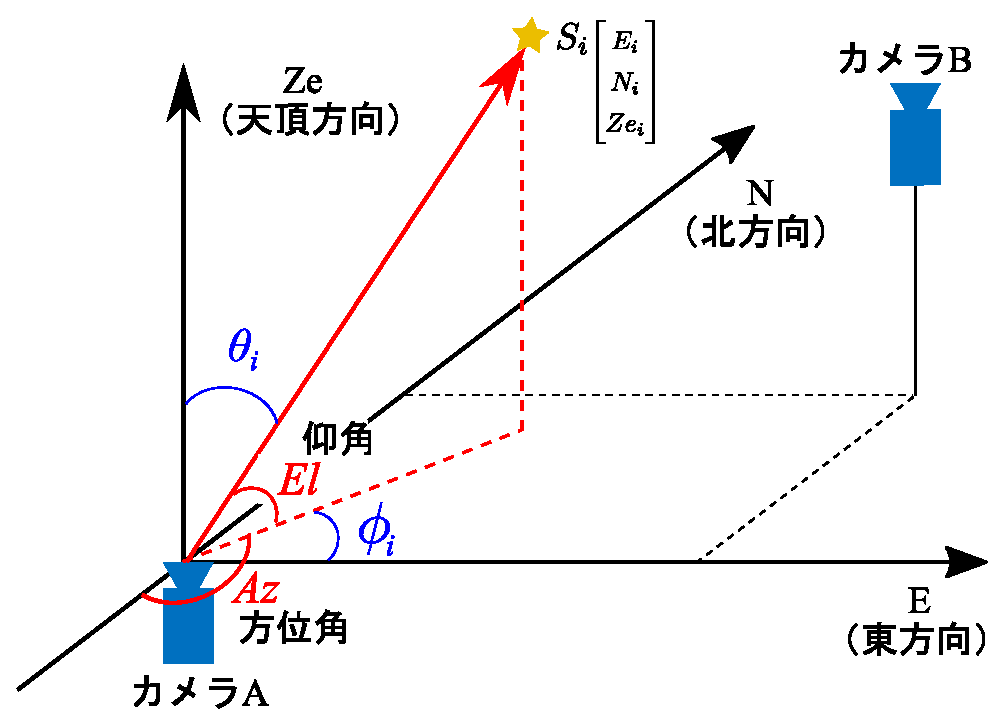
\includegraphics[width=9cm]{./chap3/eps/END2star.eps}
\caption{���E���W�n�ɂ����鐯�ւ̕����x�N�g���̎Z�o}
\label{fig:world_vector}
\end{center}
\end{figure}

\clearpage


���E���W�n�ɂ����鐯�̕����x�N�g�������N�e�B�t�@�C�h���W�n�ɂ���������x�N�g���֕ϊ����邽�߂ɁC\ref{ssec:position}�ڂ�GPS�̈ʒu��񂩂�Z�o�����J�����Ԃ̕��ʊp$\alpha$�ƋŠp$\beta$���g�p����D
���N�e�B�t�@�C�h���W�n�ɂ����鐯�̕����x�N�g���̎Z�o��}\ref{fig:ricthi_vector}�Ɏ����D�}����X���CY���CZ���̓��N�e�B�t�@�C�h���W�n�̍��W���ł���D
�}\ref{fig:ricthi_vector}���番����悤�ɁCENZe���W�n�����N�e�B�t�@�C�h���W�n�ւƕϊ����邽�߂ɂ�Ze���܂���$\alpha$��]������CN���܂���-$\beta$��]����΂悢�D
�����Ń��N�e�B�t�@�C�h���W�n�ɂ�����$S_i$�Ɍ����������̒P�ʃx�N�g��$\mathbf{m_{\it i}}$�́C��(\ref{eq:Ry})�Ǝ�(\ref{eq:Rz})�Œ�`������]�s��ƁC��(\ref{eq:xyz})�ŎZ�o����ENZe���W�n�ɂ�����$S_i$�̕����̒P�ʃx�N�g�� $(E_i, N_i, Ze_i)^T$��p����
�ȉ��̎�(\ref{eq:ricthi_vector})�ɂ���ĎZ�o�����D

\begin{equation}
\mathbf{m_{\it i}}=
\begin{bmatrix}
X_i\\
Y_i\\
Z_i
\end{bmatrix}
=\mathbf{R}(N, -\beta)\mathbf{R}(D, \alpha)
\begin{bmatrix}
E_i\\
N_i\\
Ze_i
\end{bmatrix}
\label{eq:ricthi_vector}
\end{equation}
%\clearpage

\vspace{2cm}


\begin{figure}[hbp]
\begin{center}
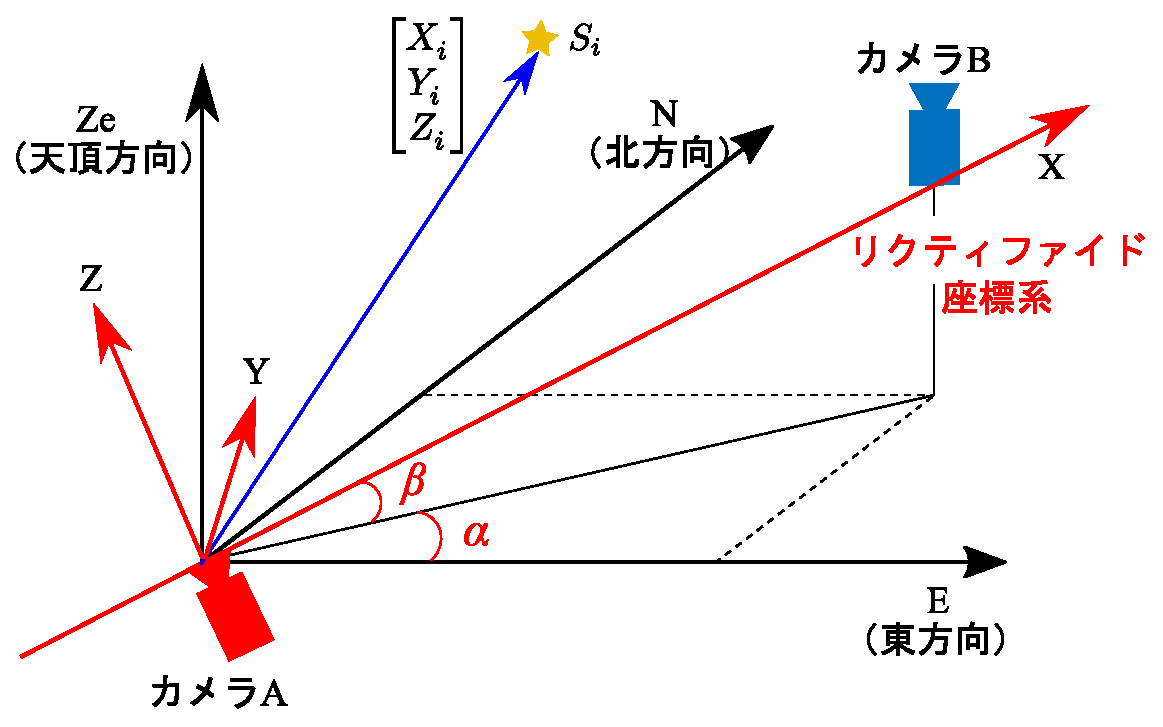
\includegraphics[width=11cm]{./chap3/eps/ricthi_vector.eps}
\caption{���N�e�B�t�@�C�h���W�n�ɂ����鐯�ւ̕����x�N�g���̎Z�o}
\label{fig:ricthi_vector}
\end{center}
\end{figure}

\clearpage


�����ŁC���N�e�B�t�@�C�h���W�n����J�������W�n�ւ̉�]�s��$\mathbf{R}$��$N$�‚̐��S�Ăɂ����Ď�(\ref{eq:nRm})�𖞂����s��ł���D
����āC���N�e�B�t�@�C�h���W�n�ɂ�����$S_i$�̕����x�N�g��$\mathbf{m_{\it i}}$�ƁC�J�������W�n�ɂ�����$S_i$�̕����x�N�g��$\mathbf{n_{\it i}}$����C��]�s��$\mathbf{R}$��p�����Ƃ��̌덷$\|\mathbf{n}_i - \mathbf{R}\mathbf{m}_i\|^2$�̑��a���ŏ��ƂȂ�悤��
��]�s��$\mathbf{R}$�����߂�D
�{�����ł͎�(\ref{eq:Restimate})�Ŏ����悤�ɓ��ْl������p���āC�J����A�C�J����B�̏ꍇ���ꂼ��ɂ�����$\mathbf{R}$�𐄒肷��D

\begin{equation}
\begin{split}
\min\sum_{i=1}^\mathbf{n} \|\mathbf{n}_i - \mathbf{R}\mathbf{m}_i\|^2 \\
= \min\|\mathbf{N} - \mathbf{RM} \|^2 \\
������ \mathbf{N} = (\mathbf{n}_1, \mathbf{n}_2, ..., \mathbf{n}_n), \mathbf{M} = (\mathbf{m}_1, \mathbf{m}_2, ..., \mathbf{m}_n)\\
\\
������\|\mathbf{N} - \mathbf{RM} \|^2\\
= tr((\mathbf{N}-\mathbf{RM})^T(\mathbf{N}-\mathbf{RM}))\\
=tr(\mathbf{N}^T\mathbf{N})+tr(\mathbf{M}^T\mathbf{M})-2tr(\mathbf{N}^T\mathbf{RM})�@����\\
\min\|\mathbf{N} - \mathbf{RM} \|^2 ���@\max(tr(\mathbf{N}^T\mathbf{RM}))�ƂȂ�\\
\\
\mathbf{MN}^T = \mathbf{U\Sigma V}^T�Ƃ����\\
tr(\mathbf{N}^T\mathbf{RM}) = tr(\mathbf{RMN}^T)\\
=tr(\mathbf{RU\Sigma V}^T)\\
=tr(\mathbf{V}^T\mathbf{RU\Sigma V}) \leq tr(\Sigma)�@���\\
\mathbf{V}^T\mathbf{RU} = \mathbf{I}_3�@�̂Ƃ��@tr(\mathbf{N}^T\mathbf{RM})�� \max �ƂȂ�\\
����ā@\mathbf{R} = \mathbf{VU}^T
\end{split}
\label{eq:Restimate}
\end{equation}


\textcolor{red}{������}

%\begin{equation}
% \mathbf{R}=\argmin_{R}E
%\label{eq:saisyouR}
%\end{equation}





\clearpage
%%%%%%%%%%%%%%%%%%%%%%%%%%%%%%%%%%%%%%%%%%%%%%%%%%%%%%%%%%%%%%%%%%%%%%%%%%%%%%%%%%%%%%%%%%%%%%%%%%%%%%%%%%%%%%%%%%%%%%%%%%%%%%%%%%%
\section{���N�e�B�t�@�C�h���W�n�摜�ւ̕ϊ�}
\label{sec:translation}

�{�߂ł́C\ref{sec:calibration}�߂ɂĐ��肵���p�����[�^����ɁC�摜��
\ref{sec:rectified}�߂Œ�`�������N�e�B�t�@�C�h���W�n�ɏ]�����s���摜�ւƕϊ������@�ɂ‚��ďq�ׂ�D
�摜�̕ϊ��ɂ́C\ref{sec:external_parameter}���ɂĐ��肵����]�s��$\mathbf{R}$��p����D
�ϊ���̉摜��̔C�ӂ̓_��$(U, V)$�C����ɑΉ�����ϊ��O�̉摜��̓_��$(u, v)$�Ƃ���D
\ref{sec:internal_parameter}���ɂĐ��肵���摜���S$(C_u, C_v)$�C�c�݊֐�$g(r)$���g�p���C
��(\ref{eq:ocamcalib1})--��(\ref{eq:ocamcalib_k})����C$(u, v)$�ɑΉ�����3���������x�N�g��$\mathbf{n}$����(\ref{eq:n_vector})�̂悤�ɎZ�o�”\�ł���D\\

\begin{equation}
\mathbf{n}=\frac{1}{\sqrt{r^2 +g(r)^2}}
\begin{bmatrix}
u-C_u\\
v-C_v\\
g(r)
\end{bmatrix}
=
\begin{bmatrix}
x(u,v)\\
y(u,v)\\
z(u,v)
\end{bmatrix}
\label{eq:n_vector}
\end{equation}


�����ŁC��]�s��$\mathbf{R}$�̓��N�e�B�t�@�C�h���W�n����J�������W�n�֕ϊ�����s��ł��邽�߁C
��(\ref{eq:nRm})�����藧�D
����ĉ�]�s��$\mathbf{R}$�̋t�s��$\mathbf{R}^{-1}$����(\ref{eq:rotation_matrix_Inver})�ŕ\���ƁC
$(U, V)$�ɑΉ�����3���������x�N�g��$\mathbf{m}$�͎�(\ref{eq:m_vector})�ɂ�蓾���C
��(\ref{eq:m_vector})����ɍ��W�\��$(\theta�C\phi)$�͎�(\ref{eq:theta_phi})�ɂ��C$\mathbf{n}$�̊֐��Ƃ��ĕ\����D\\

\begin{equation}
\mathbf{R}^{-1}=
\begin{bmatrix}
r_{11} &r_{12} &r_{13}\\
r_{21} &r_{22} &r_{23}\\
r_{31} &r_{32} &r_{33}
\end{bmatrix}
=
\begin{bmatrix}
\mathbf{r}_{1}\\
\mathbf{r}_{2}\\
\mathbf{r}_{3}
\end{bmatrix}
�C\mathbf{r}_{k}=
\begin{bmatrix}
r_{k1} &r_{k2} &r_{k3}
\end{bmatrix}
�ik=1,2,3�j
\label{eq:rotation_matrix_Inver}
\end{equation}

\begin{equation}
\mathbf{m}=
\begin{bmatrix}
\sin\theta\cos\phi\\
\sin\theta\sin\phi\\
\cos\theta
\end{bmatrix}
=\mathbf{R}^{-1}\mathbf{n}=
\begin{bmatrix}
\mathbf{r}_{1}\mathbf{n}\\
\mathbf{r}_{2}\mathbf{n}\\
\mathbf{r}_{3}\mathbf{n}
\end{bmatrix}
\label{eq:m_vector}
\end{equation}

%\begin{equation}
%\theta= \arccos(\mathbf{r}_{3}\mathbf{n})= f(\mathbf{n}), \phi=\arctan(\frac{\mathbf{r}_{2}\mathbf{n}}{\mathbf{r}_{1}\mathbf{n}})=g(\mathbf{n})
%\label{eq:theta_phi}
%\end{equation}

\begin{equation}
\begin{bmatrix}
\theta\\
\phi
\end{bmatrix}
=
\begin{bmatrix}
\cos^{-1}(\mathbf{r}_{3}\mathbf{n})\\
\tan^{-1}({\mathbf{r}_{2}\mathbf{n}}/{\mathbf{r}_{1}\mathbf{n}})
\end{bmatrix}
=
\begin{bmatrix}
h(\mathbf{n})\\
i(\mathbf{n})
\end{bmatrix}
\label{eq:theta_phi}
\end{equation}


�܂��C�g�p����J�����̓L�����u���[�V�������������Ă��邽�߁C
�����̓��ˊp$\theta$�Ɠ��e�_����摜���S�܂ł̋���$r'$�Ƃ̊֌W�͊��m�ł���D
�����$r'$����(\ref{eq:theta_r})�̂悤��$\theta$�ŕ\�����Ƃ��ł���D\\

\begin{equation}
r' = j(\theta)
\label{eq:theta_r}
\end{equation}


\clearpage
��(\ref{eq:fisheye_uv})�C��(\ref{eq:theta_r})����C$(U, V)$�͎�(\ref{eq:UV_uv})�ɂ��$(\theta�C\phi)$�̊֐��ŕ\����D\\

\begin{equation}
\begin{bmatrix}
U\\
V
\end{bmatrix}
=
\begin{bmatrix}
C_u+r'\cos\phi\\
C_v+r'\sin\phi
\end{bmatrix}
=
\begin{bmatrix}
s(\theta,\phi)\\
t(\theta,\phi)
\end{bmatrix}
\label{eq:UV_uv}
\end{equation}

�ȏ�̎�(\ref{eq:n_vector})--��(\ref{eq:UV_uv})����C�ϊ���̓_�ϊ���̓_$(U, V)$�ƁC�ϊ��O�̓_$(u, v)$�Ƃ̑Ή����Z�o�ł��邽�߁C
���N�e�B�t�@�C�h���W�n�ɏ]���摜���擾���邱�Ƃ��”\�ł���D\\

���N�e�B�t�@�C�h���W�n�ɏ]���摜�֕ϊ��O�̉摜�̗��}\ref{fig:trans_in}�C�ϊ���̉摜�̗��}\ref{fig:trans_out}�Ɏ����D
�J����A�C�J����B�ŎB�e���ꂽ�摜���̃I�[�����`���ڎ��ł��ꂼ���r����ƁC
�ϊ��O�̐}\ref{fig:trans_in}�ɂ����Ă݂͂͌��Ɋp�x���قȂ��Ă������C
�ϊ���̐}\ref{fig:trans_out}�ɂ����Ă�2���̉摜���̃I�[�����̌�������v���Ă��邱�Ƃ��m�F�ł���D

\clearpage

\begin{figure}[htb]
  \centering
  \subfigure[�J����A]{
    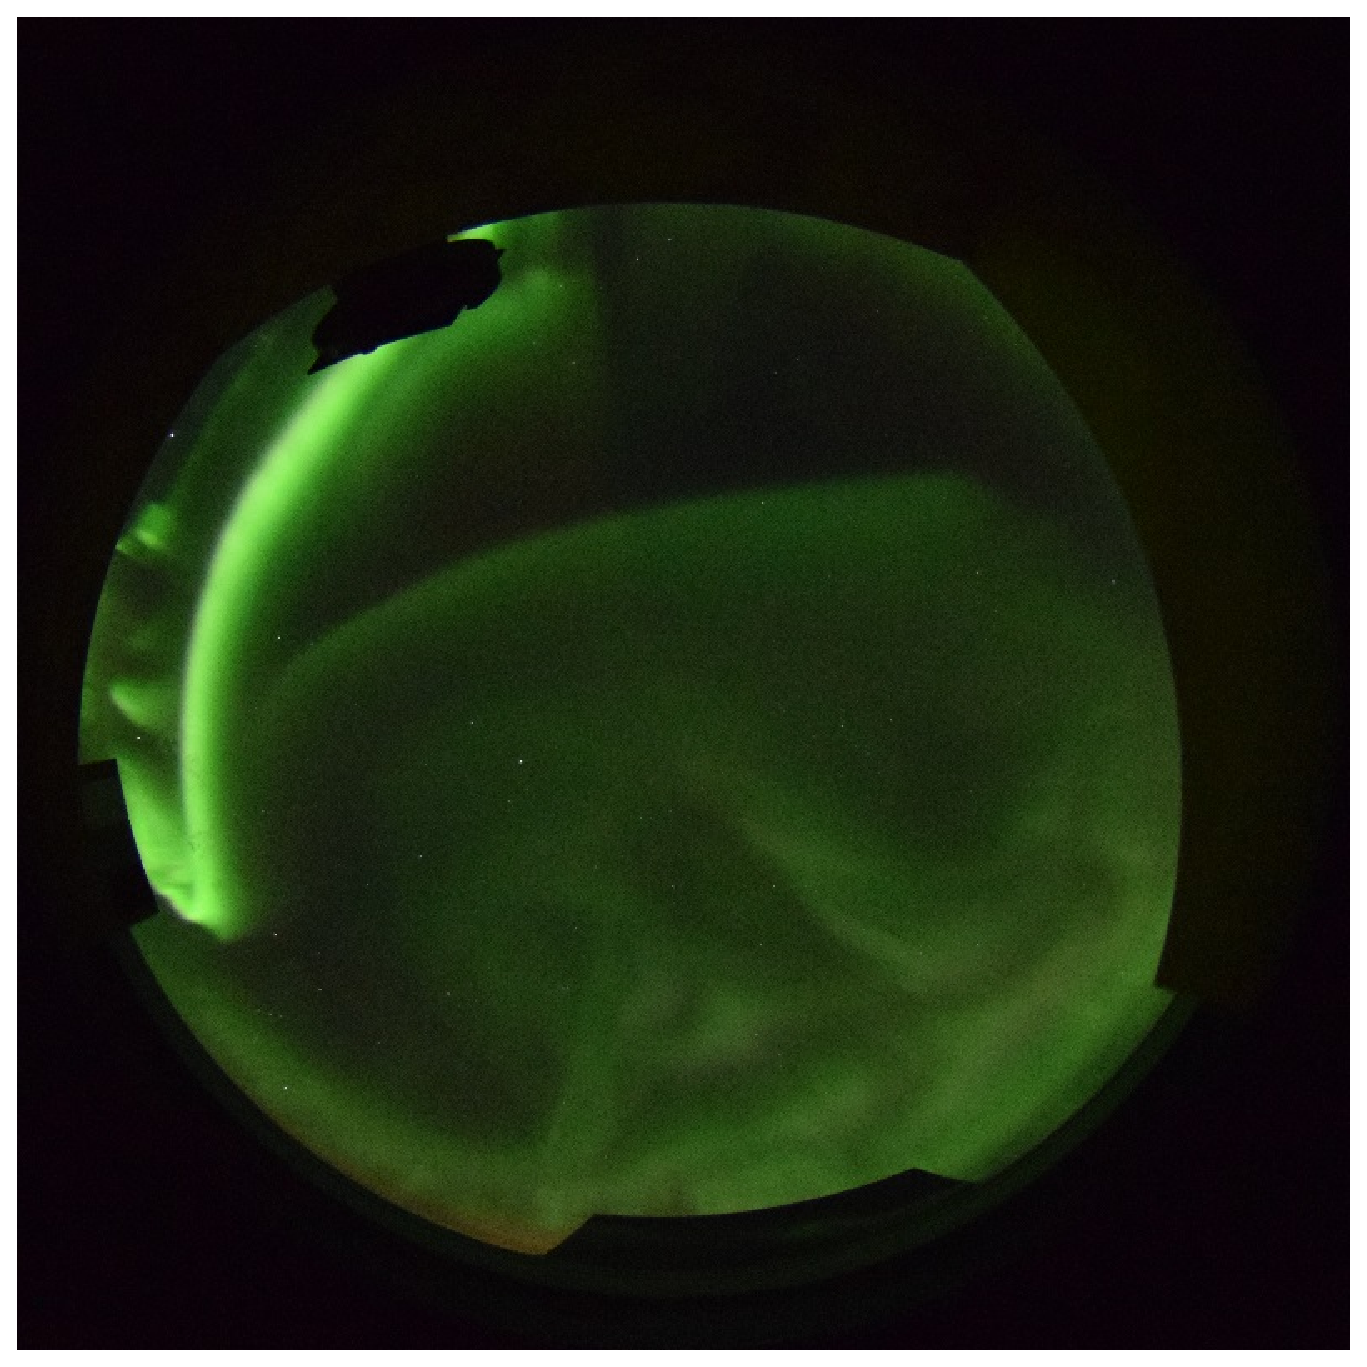
\includegraphics[width=5cm]{./chap3/eps/019_ori_L.eps}
  \label{fig:trans_in1}}
  \subfigure[�J����B]{
    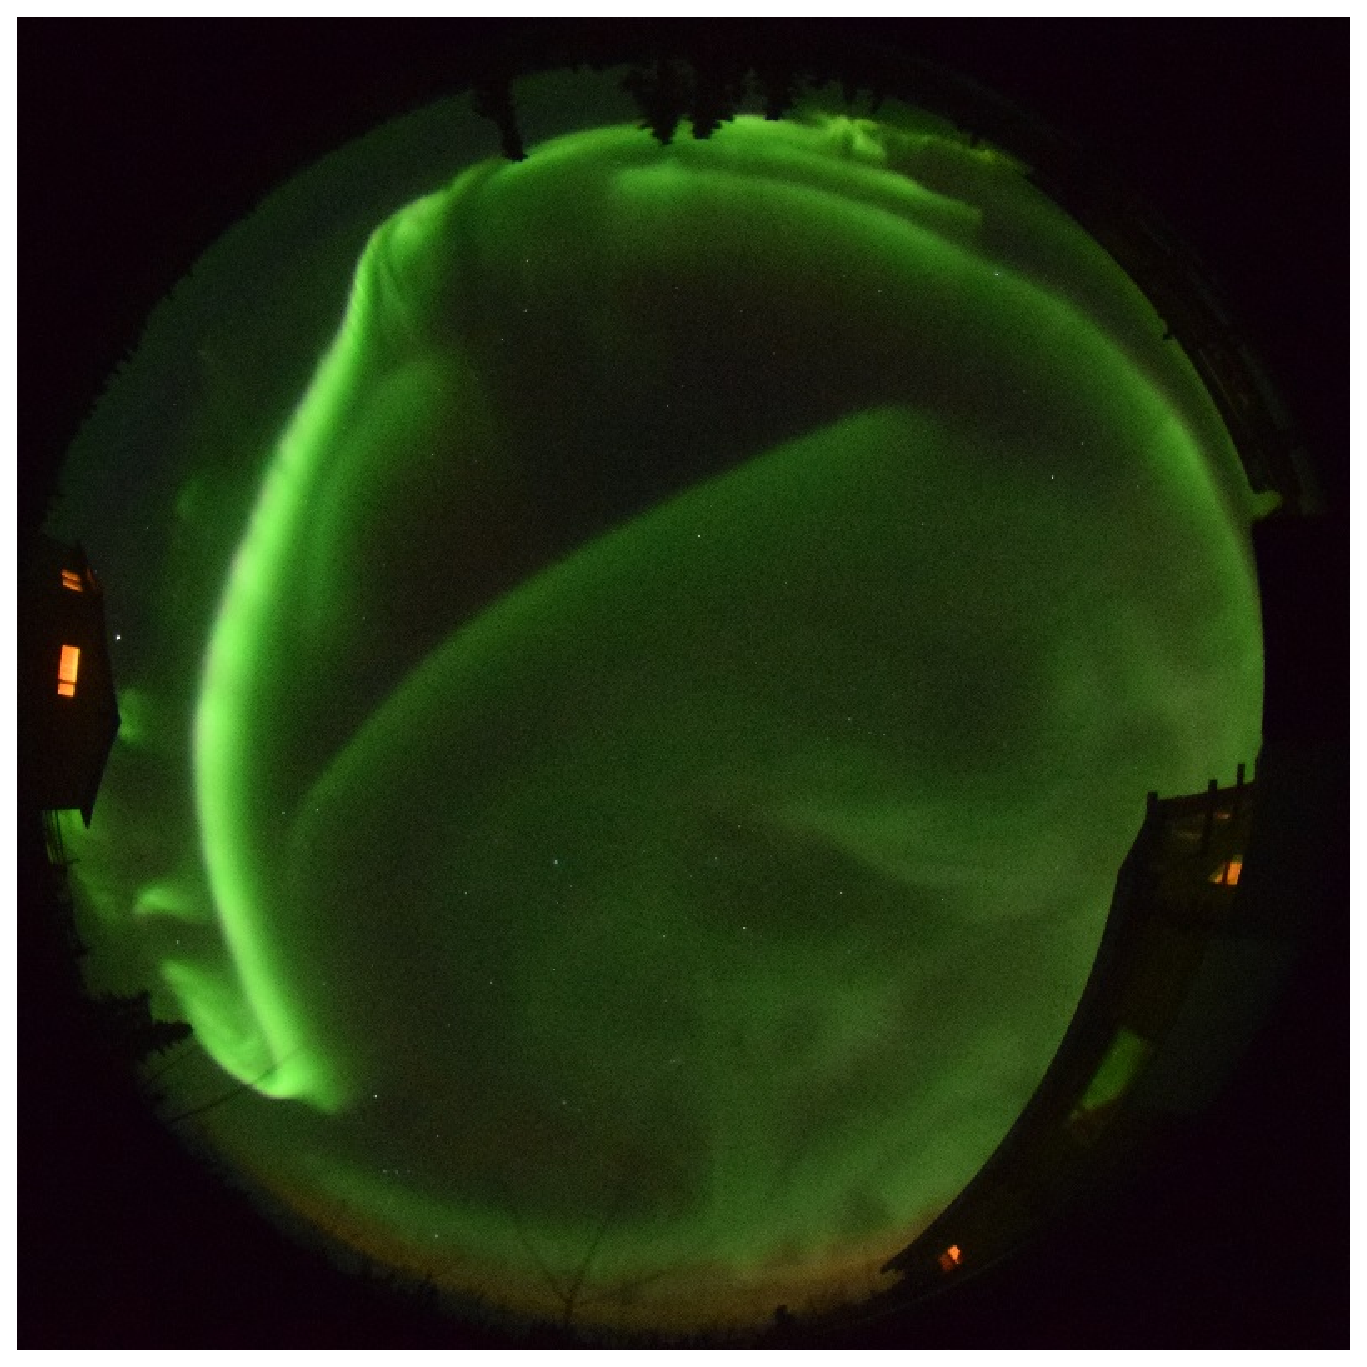
\includegraphics[width=5cm]{./chap3/eps/019_ori_R.eps}
  \label{fig:trans_in2}}
  \caption{���N�e�B�t�@�C�h���W�n�ւ̕ϊ��O�摜}
  \label{fig:trans_in}
\end{figure}


\begin{figure}[htb]
  \centering
  \subfigure[�J����A]{
    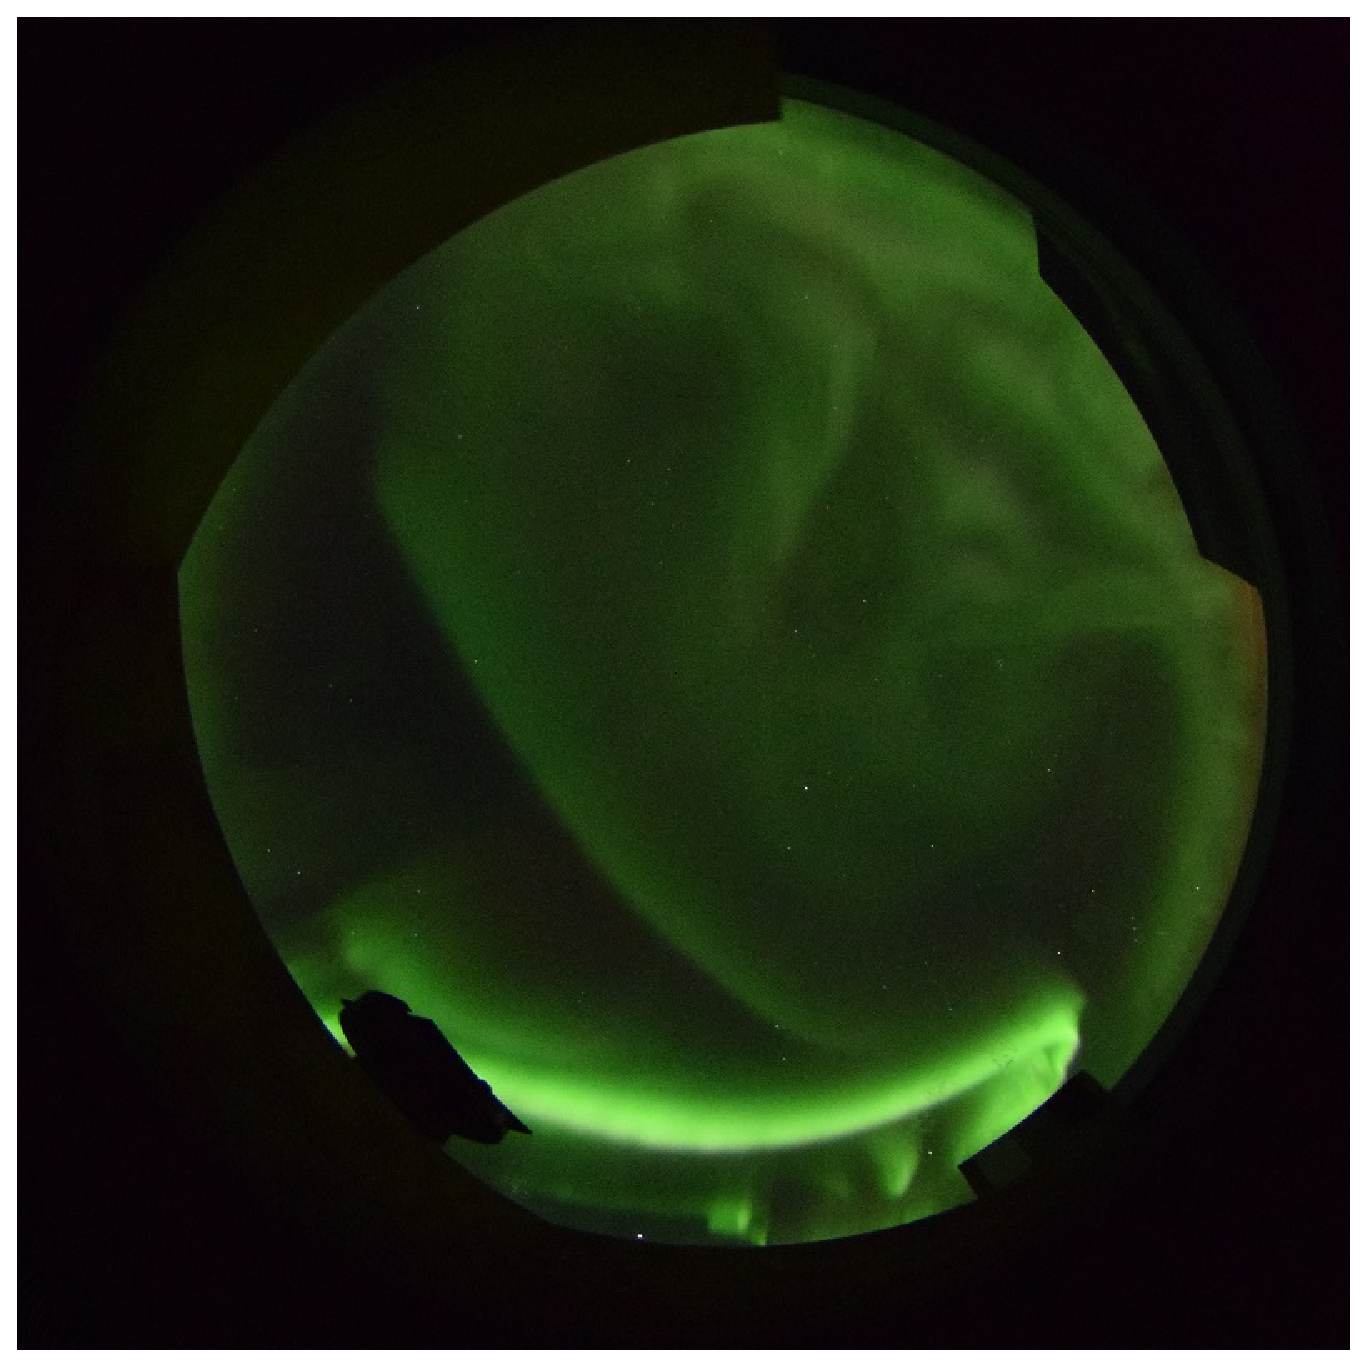
\includegraphics[width=5cm]{./chap3/eps/019_trans_L.eps}
  \label{fig:trans_out1}}
  \subfigure[�J����B]{
    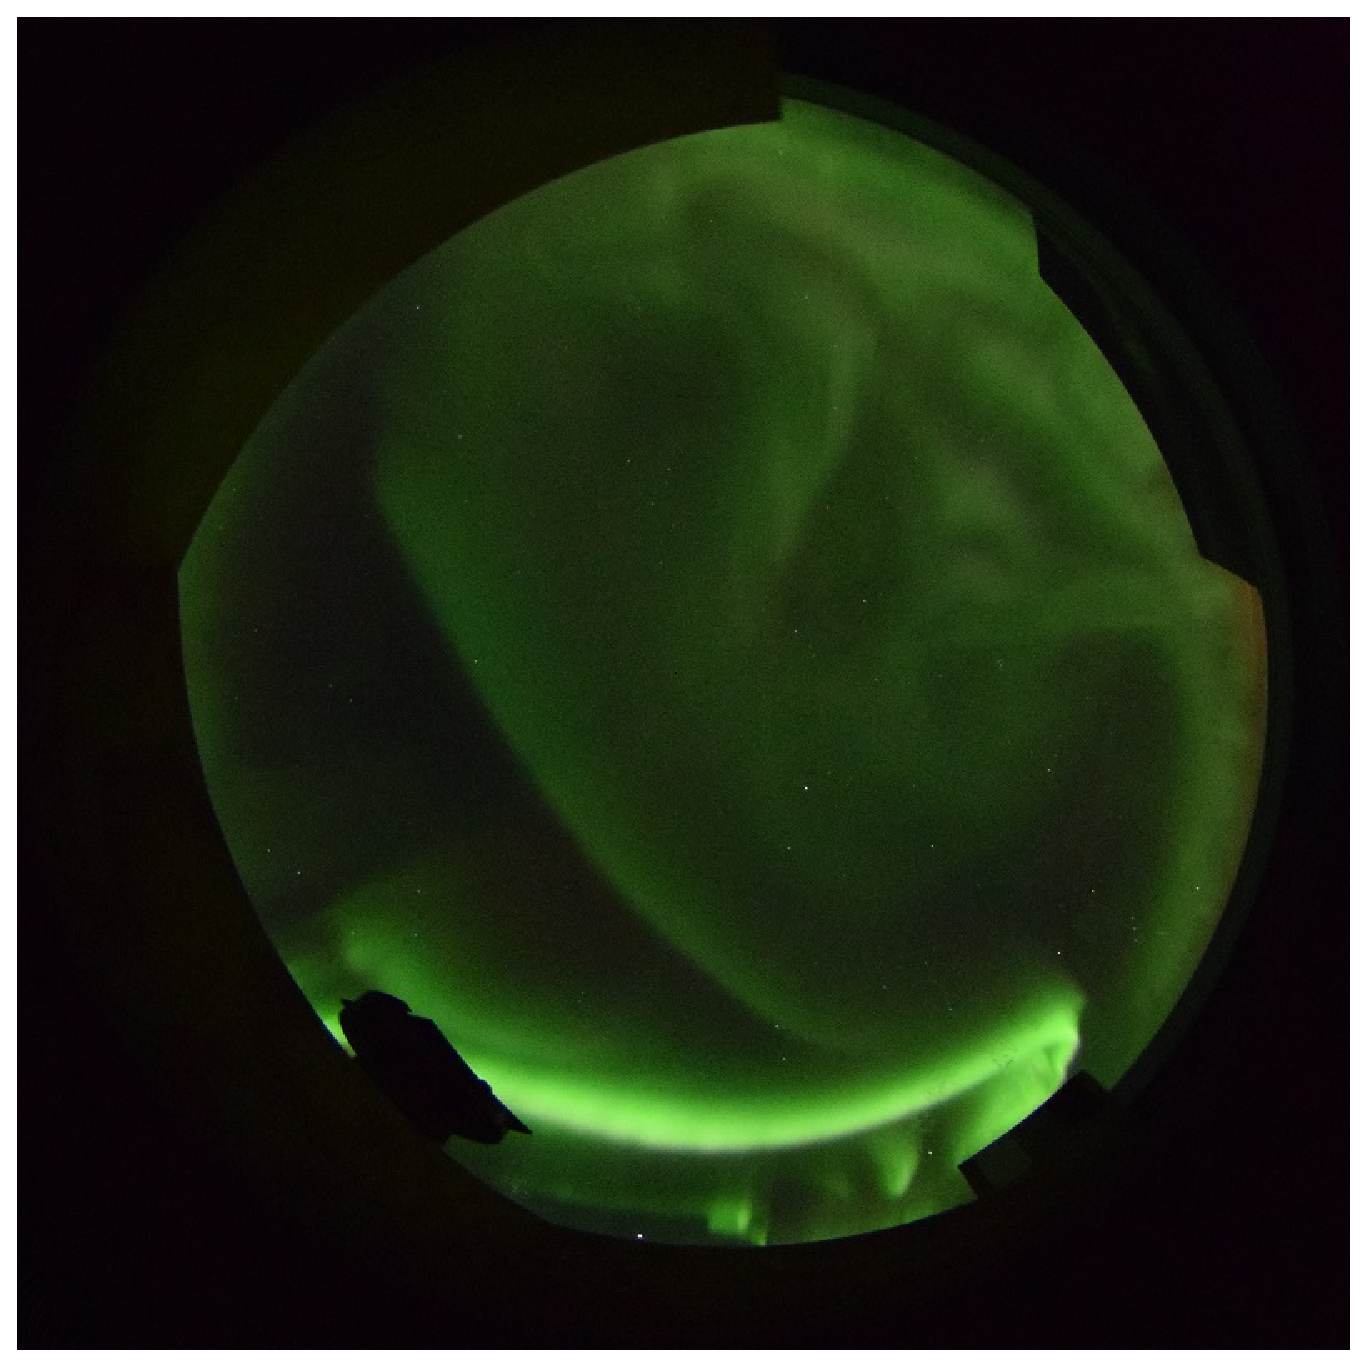
\includegraphics[width=5cm]{./chap3/eps/019_trans_L.eps}
  \label{fig:trans_out2}}
  \caption{���N�e�B�t�@�C�h���W�n�ւ̕ϊ���摜}
  \label{fig:trans_out}
\end{figure}

\clearpage

%�i�摜�����ւ��H�j
%%%%%%%%%%%%%%%%%%%%%%%%%%%%%%%%%%%%%%%%%%%%%%%%%%%%%%%%%%%%%%%%%%%%%%%%%%%%%%%%%%%%%%%%%%%%%%%%%%%%%%%%%%%%%%%%%%%%%%%%%%%%%%%%%%%
\section{����摜���瓧�����e�摜�ւ̕ϊ�}
\label{sec:undistortion}

����J�����ɂ��擾����摜�́C���჌���Y�̐����ɂ��c�݂�L����D�{�߂ł͎擾�摜���狛�჌���Y�ɂ��c�݂��������������e�ˉe�摜�֕ϊ�����D
�{�����Ŏg�p���鋛�჌���Y�̘c�݂�\ref{sec:internal_parameter}���Ő��肵���c�݊֐��Ɋ�Â��Ă���D
���ˌ��Ɖ摜��̓��e�_�̊֌W�̓L�����u���[�V�����ɂ���Ď�(\ref{eq:theta_r})�̂悤�Ɋ��m�ł���Ƃ���D\\

����摜���瓧�����e�摜�ւ̕ϊ��̗l�q��}\ref{fig:fisheye_ray}�C�}\ref{fig:hoseimen}�Ɏ����D
�}\ref{fig:fisheye_ray}�C�}\ref{fig:hoseimen}�͓������e�摜���ʂ��œ_����$Z_v$�̋����ɂ��邫�C
�������e�摜��̓��e�_�Ƌ���摜��̓��e�_���֌W�t���Ă���}�ł���D
����摜��̔C�ӂ̓_$(x_f, y_f)$���������e�摜���$(x_p, y_p)$�ƂȂ�Ƃ���D\\

\begin{figure}[b]
\begin{center}
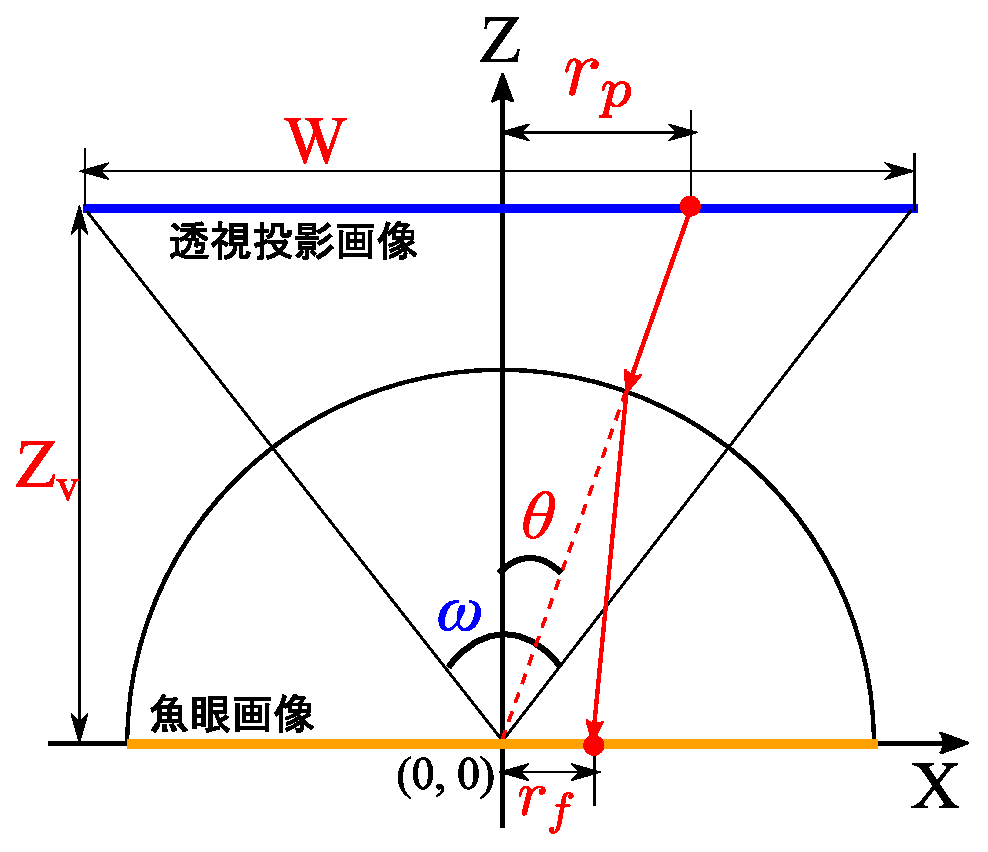
\includegraphics[width=7cm]{./chap3/eps/Fisheye2perspective.eps}
%\vspace{-0.5cm}
\caption{�������e�摜��̓_���狛�჌���Y�ւ̓��ˌ��̗l�q}
\label{fig:fisheye_ray}
\end{center}
\end{figure}

\begin{figure}[tb]
\begin{center}
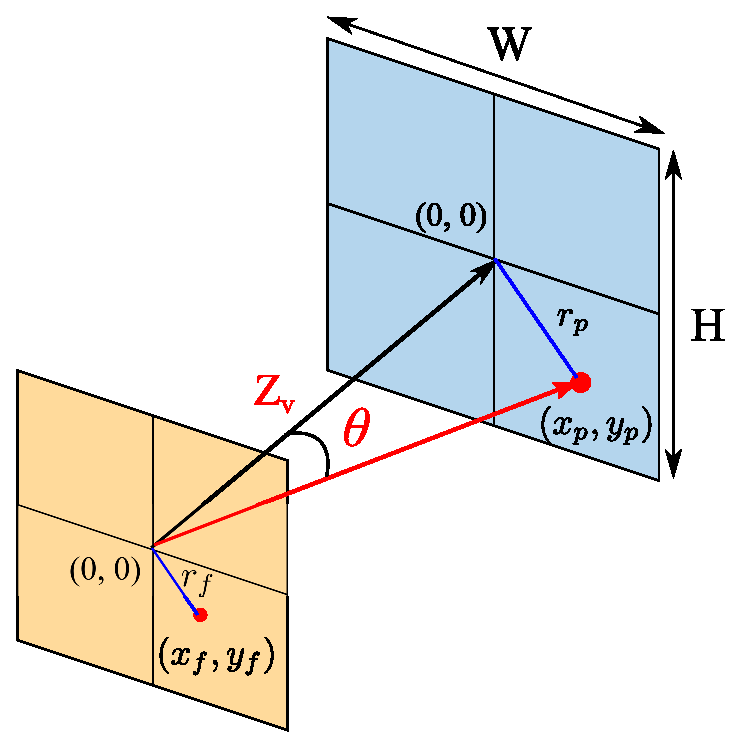
\includegraphics[width=7cm]{./chap3/eps/Fisheye2perspective2.eps}
\caption{�������e�摜��̓_�ƑΉ����鋛��摜��̓_�̊֌W}
\label{fig:hoseimen}
\end{center}
\end{figure}

�c�݂̕␳�ɍۂ��Ă܂��C����摜���瓧�����e�摜�ւƕϊ������p�͈͂��߂�D
�ʏ틛��摜�͉摜���S���痣���قǘc�݂��傫���␳������ɂȂ�D
�����Ōv�����x�̒ቺ������邽�߁C�{�����ł͉�p���ɂ߂đ傫���̈�͌v���͈͊O�Ƃ���D
�{�߂ł͔C�ӂ̉�p$\omega$ �͈̔͂ɂĕ␳�ʓW�J���s���Ƃ���D
���ɁC�␳�ʓW�J��̉摜�̍����C�������ꂼ��H�CW�Ƃ��C�}\ref{fig:fisheye_ray}�̂悤�ɏœ_����$Z_v$��ݒ肷��D
�������e�摜�ւ̕ϊ��́C�������e�摜��̍��W$(x_f, y_f)$�ɑΉ����鋛��摜��̓_$(x_p, y_p)$���Z�o���邱�Ƃōs���D
���჌���Y�ɂ��c�݂͉摜���S������˕����݂̂ł��邱�Ƃ���C����摜�̒��S����C�ӂ̓_$(x_f, y_f)$�܂ł̋�����$r_f$�C�������e�摜�̒��S����Ή�����_$(x_p, y_p)$�܂ł̋�����$r_p$�Ƃ���ƁC
�}\ref{fig:fisheye_ray}�C�}\ref{fig:hoseimen}���C$(x_f, y_f)$�C$(x_p, x_p)$�͎��̂悤�Ȋ֌W�����D

\begin{eqnarray}
\left[\begin{array}{cc}x_f\\y_f \end{array}\right] = \frac{r_f}{r_p} \left[\begin{array}{cc}x_p \\ y_p \end{array}\right]
\label{eq:XY}
\end{eqnarray}

����āC�������e�摜��̓_$(x_p, y_p)$�ɑΉ����鋛��摜��̓_$(x_f, y_f)$�����߂邽�߂ɂ�$r_f$�C$r_p$�̒l�����܂�Ηǂ��D
�����ŁC$r_p$�͐}\ref{fig:fisheye_ray}���C����(\ref{eq:R})�ɂ�苁�܂�D

\begin{eqnarray}
r_p = \sqrt{ x_p^2 + y_p^2}
\label{eq:R}
\end{eqnarray}

�܂��C$r_f$�͎�(\ref{eq:theta_r})���C$\theta$�̒l����܂�ΎZ�o�ł���D$\theta$�̒l�͎���(\ref{eq:theta})�C(\ref{eq:Zv})�ɂ��Z�o�����D
����������$r_f$�͎�(\ref{eq:r_p})�ɂ��C$x_p$�C$y_p$�C$Z_v$�̊֐��ŕ\�����D

\begin{eqnarray}
\theta = \cos^{-1} \frac{Zv}{\sqrt{ x_p^2 + y_p^2 + Z_v^2} }
\label{eq:theta}
\end{eqnarray}

\begin{eqnarray}
Z_v = \frac{W}{ 2\tan{\frac{\omega}{2}} }
\label{eq:Zv}
\end{eqnarray}

\begin{eqnarray}
r_f = j(x_p,y_p,Z_v)
\label{eq:r_p}
\end{eqnarray}

�ȏ�̊֌W���Ɋ�Â��C����摜���瓧�����e�摜�ւ̕ϊ����s���D










����摜�̘c�ݏ������s���O�̉摜�̗��}\ref{fig:before_expansion_120}�C���̉摜�𓧎����e�摜�ւƕϊ��������ʉ摜��}\ref{fig:after_expansion_120}�Ɏ����D
�}\ref{fig:before_expansion_120}���ɂ����ċ��჌���Y�ɂ��c��ł��������C�}\ref{fig:after_expansion_120}�̕␳�ʓW�J��̉摜���ł͒����ɂȂ��Ă��邱�Ƃ��m�F�ł���D


\begin{figure}[htb]
\begin{center}
\includegraphics[width=7cm]{./chap3/tmp/before_expansion.eps}
\caption{�␳�ʓW�J�O�̉摜�̗�i����J�����ł̎擾�摜�j}
\label{fig:before_expansion_120}
\end{center}
\end{figure}

\vspace{-0.5cm}

\begin{figure}[htb]
\begin{center}
\includegraphics[width=7cm]{./chap3/tmp/after_expansion.eps}
\caption{�␳�ʓW�J��̉摜�̗�}
\label{fig:after_expansion_120}
\end{center}
\end{figure}

\clearpage

%%%%%%%%%%%%%%%%%%%%%%%%%%%%%%%%%%%%%%%%%%%%%%%%%%%%%%%%%%%%%%%%%%%%%%%%%%%%%%%%%%%%%%%%%%%%%%%%%%%%%%%%%%%%%%%%%%%%%%%%%%%%%%%%%%%
\section{������}

�{�͂ł́C����J�����Ŏ擾�����摜�ɂ���ăI�[������3�����v�����s�����߂ɗp������W�n��K�v�ȃp�����[�^�C�摜�����ɂ‚��ďq�ׂ��D

�܂�\ref{sec:gaiyou2}�߂ł͖{�͂ōs���摜�����̊T�v�ɂ‚��ďq�ׁC\ref{sec:rectified}�߂Ŗ{�����ŋ���摜�΂𕽍s�X�e���I�y�A�Ƃ��Ĉ������߂ɒ�`������W�n�ɂ‚��ďq�ׂ��D

\ref{sec:fisheye_model}�߂ł́C��ʓI�ȃJ�����Ƌ���J�����̈Ⴂ�ɂ‚��ďq�ׂ���C���჌���Y�ɂ��c�݂̃��f���ɂ‚��Đ������C�{�����ŗp���鋛��J�����̃��f���ɂ‚��ďq�ׂ��D

\ref{sec:calibration}�߂Ŗ{�����ɂ�����摜�����ɕK�v�ȃp�����[�^�ƁC�����̐�����@�ɂ‚��ďq�ׂ��D

\ref{sec:translation}�߂ł́C���͉摜�΂𕽍s�X�e���I�摜�΂ւƕϊ�����摜������@�ɂ‚��ďq�ׂ��D

%���̍��W�n�ւ̉摜�̕ϊ����@�ɂ‚��ďq�ׂ�D�ϊ��ɂ�\ref{sec:calibration}�߂Ő��肵���p�����[�^��p����D

�Ō��\ref{sec:undistortion}�߂ł́C���͉摜���狛�჌���Y�ɂ��c�݂���菜���������e�摜�ւƕϊ������@�ɂ‚��ďq�ׂ��D

���͂ł́C���s������c�݂̏������ꂽ�I�[�����摜����͂Ƃ��C
�I�[������3�����v�����s��3�����Ž��������@�ɂ‚��ďq�ׂ�D
%�Ō��\ref{sec:backsubtraction}�߂ł́C�����_���o�̂��߂ɉ摜������I�[�����̈�𒊏o����w�i�����ɂ‚��ďq�ׂ�D
\clearpage



%%%%%%%%%%%%%%%%%%%%%%%%%%%%%%%%%%%%%%%%%%%%%%%%%%%%%%%%%%%%%%%%%%%%%%%%%%%%%%%%%%%%%%%%%%%%%%%%%%%%%%%%%%%%%%%%%%%%%%%%%%%%%%%%%%%
%%% Local Variables:
%%% mode: katex
%%% TeX-master: "../thesis"
%%% End:

\chapter{位置推定}
\thispagestyle{empty}
\label{chap4}
\minitoc

\newpage
%%%%%%%%%%%%%%%%%%%%%%%%%%%%%%%%%%%%%%%%%%%%%%%%%%%%%%%%%%%%%%%%%%%%%%%%%%%%%%%
%==============================================================================
% 4.1
%==============================================================================
\section{はじめに}

本章では,位置$\bm{P}$を推定する手法について述べる.

4.2節にて,手法の概要について述べる.

4.3節にて,特徴量の計算について述べる.

4.4節にて,$xy$座標の推定方法について述べる.

4.5節にて,$z$座標の推定方法について述べる.


\clearpage
%==============================================================================
% 4.2
%==============================================================================
\section{位置推定の概要}

位置推定では,各エッジ点とそれに対応する単位球面勾配ベクトル,姿勢$\bm{O}$,ラインマップからカメラの位置$\bm{P}$を推定する.
図\ref{fig:derotation}に示すように,ワールド座標系から姿勢$\bm{O}$の分ずれているカメラ座標系$x_{\rm{sph}}y_{\rm{sph}}z_{\rm{sph}}$を$\bm{O}^{-1}$回転させることでワールド座標系と向きが一致した状態に変換して位置を推定する.変換後のカメラ座標系を$x'_{\rm{sph}}y'_{\rm{sph}}z'_{\rm{sph}}$とする.
\\

\begin{figure}[b]
 \begin{center}
 \includegraphics[width=0.85\columnwidth]{./chap4/fig/derotation.png}
 \caption{ワールド座標系の向きと一致させるようなカメラ座標系の回転}
 \label{fig:derotation}
 \end{center}
\end{figure}

位置推定では,ワールド座標系における各軸方向の直線が球面に投影されたとき,それぞれの軸方向を法線ベクトルとする大円と交わる点の分布を特徴量とする.
この特徴量は,$y'_{\rm{sph}}z'_{\rm{sph}}$平面,$x'_{\rm{sph}}z'_{\rm{sph}}$平面,$x'_{\rm{sph}}y'_{\rm{sph}}$平面のそれぞれにおける単位円上の点の集合で表される.
例えば,図\ref{fig:feature_x}に示すように,青い実線で示す$x$軸方向に伸びる直線は青い破線で示す線のように球面に投影され,この破線と$x'_{\rm{sph}}$方向を法線ベクトルとする大円の交点は$y'_{\rm{sph}}z'_{\rm{sph}}$平面における単位円上に存在する.
すべての$x$軸方向の直線について同様に交点を計算すると,$y'_{\rm{sph}}z'_{\rm{sph}}$平面における単位円上の点の集合が得られる.
これと同様に,$y$軸方向に伸びる直線から$x'_{\rm{sph}}z'_{\rm{sph}}$平面における単位円上の点の集合が得られ(図\ref{fig:feature_y}),$z$軸方向に伸びる直線から$x'_{\rm{sph}}y'_{\rm{sph}}$平面における単位円上の点の集合が得られる(図\ref{fig:feature_z}).
これらをそれぞれ,$yz$特徴量,$xz$特徴量,$xy$特徴量と呼ぶ.
これらの特徴量は各カメラ位置において一意に定まるため,推定する画像の特徴量とラインマップから計算する各位置における特徴量を比較し,最も類似度の高い位置を探索することによりカメラの位置を推定することができる.
\\

\begin{figure}[tb]
 \begin{center}
 \includegraphics[width=0.85\columnwidth]{./chap4/fig/feature_x.png}
 \caption{$x$軸方向の直線から得られる$y'_{\rm{sph}}z'_{\rm{sph}}$平面における単位円上の点の集合}
 \label{fig:feature_x}
 \end{center}
\end{figure}

\begin{figure}[tb]
 \begin{center}
 \includegraphics[width=0.85\columnwidth]{./chap4/fig/feature_y.png}
 \caption{$y$軸方向の直線から得られる$x'_{\rm{sph}}z'_{\rm{sph}}$平面における単位円上の点の集合}
 \label{fig:feature_y}
 \end{center}
\end{figure}

\clearpage

\begin{figure}[tb]
 \begin{center}
 \includegraphics[width=0.85\columnwidth]{./chap4/fig/feature_z.png}
 \caption{$z$軸方向の直線から得られる$x'_{\rm{sph}}y'_{\rm{sph}}$平面における単位円上の点の集合}
 \label{fig:feature_z}
 \end{center}
\end{figure}


ここで,各軸方向の直線から得られる特徴量は,その軸方向のカメラ移動に依存せずに定まる.
つまり,$x$軸方向の直線から得られる$yz$特徴量はカメラの$yz$座標にのみにより定まり,$y$軸方向の直線から得られる$xz$特徴量はカメラの$xz$座標にのみにより定まり,$z$軸方向の直線から得られる$xy$特徴量はカメラの$xy$座標にのみにより定まる.
これを利用して,はじめに1つの特徴量を用いて2自由度の推定を行い,次に残りの特徴量から1つを選んで残りの1自由度の推定を行うことで,2自由度の推定と1自由度の推定に分離して行う.
本研究では,はじめに$xy$特徴量を用いた2次元の探索により$xy$座標を推定し,その後$xz$特徴量と推定された$x$座標を用いた1次元の探索により$z$座標を推定した.
\\

位置推定の流れを図\ref{fig:flow4}に示す.
まず,各エッジ点とそれに対応する単位球面勾配ベクトル,姿勢$\bm{O}$から推定する画像の特徴量を計算し,$xy$特徴量と$xz$特徴量を得る.
次に,得られた$xy$特徴量とラインマップから$xy$座標の推定を行い,推定値$x^*,\ y^*$を求める.
最後に,$xz$特徴量,推定値$x^*$,ラインマップから$z$座標の推定を行い,推定値$z^*$を求める.
以上の流れで,カメラの位置$\bm{P}$の推定値$\bm{P}^*=[x^*,\ y^*,\ z^*]^{\mathrm{T}}$を得る.


\begin{figure}[tb]
 \begin{center}
 \includegraphics[width=0.7\columnwidth]{./chap4/fig/flow4.png}
 \vspace{5mm}
 \caption{位置推定の流れ}
 \label{fig:flow4}
 \end{center}
\end{figure}

\clearpage
%==============================================================================
% 4.3
%==============================================================================
\section{特徴量の計算}

\subsection{エッジ点の分類}

エッジ点とそれに対応する単位球面勾配ベクトルの組から$xy$特徴及び$xz$特徴量を得るためには,それぞれの勾配ベクトルがどの軸方向の直線によるエッジ点から得られたものかによって分類する必要がある.
姿勢を推定したあと,3平面のうち最も近い平面からの距離が閾値以上の単位勾配ベクトルをoutlierとして除去する.
残った単位球面勾配ベクトルをそれぞれ最も近い平面ごとに分類することで,元の入力画像におけるエッジ点を,どの方向の直線に属するものかで3つのグループに分類する.
分類されたエッジ点の例を図\ref{fig:classified}に示す.
赤色のエッジ点が$x$軸方向の直線によるエッジ点,緑色のエッジ点が$y$軸方向の直線によるエッジ点,青色のエッジ点が$z$軸方向の直線によるエッジ点をそれぞれ表している.
\\

\begin{figure}[b]
 \begin{center}
 \includegraphics[width=0.7\columnwidth]{./chap4/fig/edge_inlier.png}
 \caption{分類されたエッジ点}
 \label{fig:classified}
 \end{center}
\end{figure}

\clearpage

\subsection{$xy$特徴量}

$xy$座標の推定に用いる$xy$特徴量には,$z$軸方向の直線が球上に投影される直線と全天球カメラの$x_{sph}y_{sph}$平面の交点の分布$(x_k,y_k)\ (k=1, 2,..., n)$を用いる.
特徴量の計算では,4.3.1項で分類したエッジ点のうち,$z$軸方向の直線に属するものを抽出して行う.
図\ref{fig:classified}に青色で示されたエッジ点がこれに該当する.
図\ref{fig:feature_xy}に示すように,抽出されたエッジ点座標を$(u_k, v_k)\ (k=1, 2,..., n)$,画像の幅を$w$とすると,交点$(x_k,y_k)$は以下の式によって求められる.

\begin{equation}
   \left(x_k,\ y_k\right) = \left(-\sin\frac{2\pi u_k}{w},\ -\cos\frac{2\pi u_k}{w}\right).
\end{equation}

\begin{figure}[b]
 \begin{center}
 \includegraphics[width=1.0\columnwidth]{./chap4/fig/feature_xy.png}
 \vspace{5mm}
 \caption{$xy$特徴量($x_{sph}y_{sph}$平面)の計算}
 \label{fig:feature_xy}
 \end{center}
\end{figure}

\clearpage
\subsection{$xz$特徴量}
$z$座標の推定に用いる$xz$特徴量には,$y$軸方向の直線が球上に投影される直線と全天球カメラの$x_{sph}z_{sph}$平面の交点の分布$(x_k,z_k)\ (k=1, 2,..., n)$を用いる.
まず,図\ref{fig:classified}に示すエッジ画像を$x$軸回りに-90 deg回転させることで,図\ref{fig:rotated_edge}のようなエッジ画像に変換する.
特徴量の計算では,このエッジ画像内のエッジ点のうち,$y$軸方向の直線に属するものを抽出して行う.
図\ref{fig:rotated_edge}に緑色で示されたエッジ点がこれに該当する.
図\ref{fig:feature_xz}に示すように,抽出されたエッジ点座標を$(u_k, v_k)\ (k=1, 2,..., n)$,画像の幅を$w$ pixelとすると,交点$(x_k,z_k)$は以下の式によって求められる.

\begin{equation}
   \left(x_k,\ z_k\right) = \left(-\sin\frac{2\pi u_k}{w},\ -\cos\frac{2\pi u_k}{w}\right).
\end{equation}

\begin{figure}[b]
 \begin{center}
 \includegraphics[width=0.7\columnwidth]{./chap4/fig/rotated_edge.png}
 \vspace{5mm}
 \caption{$x$軸回りに-90 deg回転させたエッジ画像}
 \label{fig:rotated_edge}
 \end{center}
\end{figure}


\begin{figure}[b]
 \begin{center}
 \includegraphics[width=1.0\columnwidth]{./chap4/fig/feature_xz.png}
 \vspace{5mm}
 \caption{$xz$特徴量($x_{sph}z_{sph}$平面)の計算}
 \label{fig:feature_xz}
 \end{center}
\end{figure}


\clearpage
%==============================================================================
% 4.4
%==============================================================================
\section{$xy$座標の推定}

$xy$座標の推定では,$z$座標を固定し,2次元の最適化によって推定する.
図\ref{fig:search_xy}に座標$(x,y)$における全天球カメラを上から見た図を示す.
緑色の点が上記の方法で求めた交点,赤色の点がラインマップから求めた,座標$(x,y)$から遮蔽されることなく見えるz軸方向の直線をそれぞれ表している.
画像から全ての直線を検出できるとは限らないため交点と直線の数は必ずしも一致せず,交点の数を$n$,直線の数を$m$とする.
各交点と直線の距離を,全天球カメラ座標系においてそれぞれが成す角によって定義し,すべての交点に対する最も近い直線までの距離の二乗和が最小となるような座標$(x,y)$を推定値とする.
交点の座標を$(x_k,y_k)\ (k=1, 2,..., n)$,ラインマップにおける$z$軸方向の直線の$xy$座標を$(x_l, y_l)\ (l=1, 2,...,m)$とすると,これらの距離$d_{k,l}$は,以下の式で得られる.
\begin{equation}
   d_{k,l} = \cos^{-1}\left(\frac{x_k(x_l-x)+y_k(y_l-y)}{\sqrt{(x_l-x)^2+(y_l-y)^2}}\right).
\end{equation}

$d_{k,l}\ (l=1,2,...,m)$のうち,最も小さいものを$d_k$とする.

\begin{equation}
   d_k = \min\left(d_{k,1},\ d_{k,2},\cdots,\ d_{k,m}\right).
\end{equation}

全ての交点における$d_k$の二乗和を最小とするようなパラメータ$(x^*,y^*)$が,$xy$座標の推定値である.
この非線形最適化を,Levenberg-Marquardt法を用いて解く.

\begin{equation}
(x^*,y^*)=\argmin_{x,y} \sum_{k=1}^nd_k^2.
\label{eq:optim2}
\end{equation}

\begin{figure}[b]
 \begin{center}
 \includegraphics[width=0.6\columnwidth]{./chap4/fig/search_xy.png}
 \caption{座標$(x,y)$における全天球カメラを$z$軸方向から見た図}
 \label{fig:search_xy}
 \end{center}
\end{figure}


\clearpage
%==============================================================================
% 4.4
%==============================================================================
\section{$z$座標の推定}

$z$座標の推定では,$y$座標と前節で推定した$x$座標を固定し,1次元の最適化によって推定する.
まず,$xy$座標の推定と同様に,各交点$(x_k,z_k)$と$y$軸方向の直線の$xz$座標$(x_l,z_l)\ (l=1,2,...,m)$に対して以下の式で距離を計算する.

\begin{equation}
   d_{k,l} = \cos^{-1}\left(\frac{x_k(x_l-x^*)+z_k(z_l-z)}{\sqrt{(x_z-x^*)^2+(z_l-z)^2}}\right).
\end{equation}

$d_{k,l}\ (l=1,2,...,m)$のうち,最も小さいものを$d_k$とする.

\begin{equation}
   d_k = \min\left(d_{k,1},\ d_{k,2},\cdots,\ d_{k,m}\right).
\end{equation}

全ての交点における$d_k$の二乗和を最小とするようなパラメータ$(z^*)$が,$z$座標の推定値である.
この非線形最適化を,Levenberg-Marquardt法を用いて解く.

\begin{equation}
(z^*)=\argmin_{z} \sum_{k=1}^nd_k^2.
\label{eq:optim2}
\end{equation}


\begin{figure}[b]
 \begin{center}
 \includegraphics[width=0.6\columnwidth]{./chap4/fig/search_xz.png}
 \caption{座標$(x,z)$における全天球カメラを$y$軸方向から見た図}
 \label{fig:search_xz}
 \end{center}
\end{figure}


\clearpage
%==============================================================================
% 4.5
%==============================================================================
\section{おわりに}

本章では,位置推定手法について説明した.

4.2節にて,位置推定の概要を述べた.

4.3節にて,特徴量の計算について述べた.

4.4節にて,$xy$座標の推定方法について述べた.

4.5節にて,$z$座標の推定方法について述べる.


次章では,提案手法の有効性を検証するために行った実験について述べる.

\clearpage
%%%%%%%%%%%%%%%%%%%%%%%%%%%%%%%%%%%%%%%%%%%%%%%%%%%%%%%%%%%%%%%%%%%%%%%%%%%%%%%%%
%%%%% Local Variables:
%%%%% mode: katex
%%%%% TeX-master: "../thesis"
%%%%% End:

\chapter{実験による提案手法の評価}
\label{chap:development}
\minitoc

\thispagestyle{empty}

\newpage
%%%%%%%%%%%%%%%%%%%%%%%%%%%%%%%%%%%%%%%%%%%%%%%%%%%%%%%%%%%%%%%%%%%%%%%%%%%%%%%%%%%%%%%%%%%%%%%%%%%%%%%%%%%%%%%%%%%%%%%%%%%%%%%%%%%
\section{はじめに}
\label{sec:intro_chap5}

本章では,理学療法士の技能を利用した,起立動作の支援機器の設計と開発,ならびに評価実験について述べる.

\ref{sec:design_chap5}節にて,支援機器の設計について述べる.

\ref{sec:development_chap5}節にて,支援機器の開発について述べる.

\ref{sec:experiment_chap5}節にて,支援機器の評価を行った実験について述べる.

\ref{sec:outro_chap5}節にて,本章のまとめを述べる.

\textcolor{red}{改ページする予定です.}
%\clearpage
%%%%%%%%%%%%%%%%%%%%%%%%%%%%%%%%%%%%%%%%%%%%%%%%%%%%%%%%%%%%%%%%%%%%%%%%%%%%%%%%%%%%%%%%%%%%%%%%%%%%%%%%%%%%%%%%%%%%%%%%%%%%%%%%%%%
\section{支援機器の設計}
\label{sec:design_chap5}

本節では,起立動作の支援機器の設計について述べる.\\

\textcolor{red}{改ページする予定です.}
%\clearpage
%%%%%%%%%%%%%%%%%%%%%%%%%%%%%%%%%%%%%%%%%%%%%%%%%%%%%%%%%%%%%%%%%%%%%%%%%%%%%%%%%%%%%%%%%%%%%%%%%%%%%%%%%%%%%%%%%%%%%%%%%%%%%%%%%%%
\section{支援機器の開発}
\label{sec:development_chap5}

本節では,起立動作の支援機器の開発について述べる.\\

\textcolor{red}{改ページする予定です.}
%\clearpage
%%%%%%%%%%%%%%%%%%%%%%%%%%%%%%%%%%%%%%%%%%%%%%%%%%%%%%%%%%%%%%%%%%%%%%%%%%%%%%%%%%%%%%%%%%%%%%%%%%%%%%%%%%%%%%%%%%%%%%%%%%%%%%%%%%%
\section{評価実験}
\label{sec:experiment_chap5}

本節では,開発した支援機器の評価を行うための実験について述べる.\\

\textcolor{red}{改ページする予定です.}
%\clearpage
%%%%%%%%%%%%%%%%%%%%%%%%%%%%%%%%%%%%%%%%%%%%%%%%%%%%%%%%%%%%%%%%%%%%%%%%%%%%%%%%%%%%%%%%%%%%%%%%%%%%%%%%%%%%%%%%%%%%%%%%%%%%%%%%%%%

\section{おわりに}
\label{sec:outro_chap5}

本章では,理学療法士の技能を利用した,起立動作の支援機器の設計と開発,ならびに評価実験について述べる.

\ref{sec:design_chap5}節にて,支援機器の設計について述べた.

\ref{sec:development_chap5}節にて,支援機器の開発について述べた.

\ref{sec:experiment_chap5}節にて,支援機器の評価を行った実験について述べた.\\

開発した支援機器により健常な高齢者の起立動作を支援することが可能であることを確認した.

\clearpage
%%%%%%%%%%%%%%%%%%%%%%%%%%%%%%%%%%%%%%%%%%%%%%%%%%%%%%%%%%%%%%%%%%%%%%%%%%%%%%%%%%%%%%%%%%%%%%%%%%%%%%%%%%%%%%%%%%%%%%%%%%%%%%%%%%%
%%% Local Variables:
%%% mode: katex
%%% TeX-master: "../thesis"
%%% End:

\chapter{結論}
\thispagestyle{empty}
\label{chap6}
\minitoc

\newpage
%%%%%%%%%%%%%%%%%%%%%%%%%%%%%%%%%%%%%%%%%%%%%%%%%%%%%%%%%%%%%%%%%%%%%%%%%%%%%%%
%==============================================================================
%まとめ
%==============================================================================
\section{結論}

本論文では,直線情報に基づく全天球カメラの高速な6自由度の位置姿勢推定手法を提案した.
\vspace{\baselineskip}

第1章にて,研究背景として位置姿勢推定における全天球カメラの優位性を示し,関連する従来研究では,大域的アプローチによる全天球カメラの6自由度の位置姿勢推定として,リアルタイムのアプリケーションに適用できるような高速な手法は提案されていないことを述べた.これに基づき本研究の目的を「全天球カメラを用いた大域的なアプローチによる高速な6自由度の位置姿勢推定」と設定した.
\vspace{\baselineskip}

第2章において,本研究のアプローチについて述べた.
本研究では,位置姿勢推定において位置の推定と姿勢の推定を分離して行い,初めに姿勢を推定してから位置を推定することを述べた.
姿勢推定は消失点を用いて行い,画像の勾配のみから推定することで高速化することを述べた.
位置推定は,$xy$座標の推定と$z$座標の推定を分離してそれぞれを高速に行うことを述べた.
\vspace{\baselineskip}

第3章では姿勢推定の提案手法について詳しく説明した.
姿勢推定は,単位球面勾配ベクトルの分布とマンハッタンワールドにおける互いに直交する3平面を比較することによって行うことを説明した.
単位球面勾配ベクトルの計算は,画像内の2次元の勾配ベクトルを変換することによって行い,歪みによる勾配の計算精度の低下を抑えるために,歪みの大きい領域における勾配の計算には,入力画像を球面に変換して3次元空間において回転させた画像を用いることを述べた.
\vspace{\baselineskip}

第4章では位置推定の提案手法について詳しく説明した.
$z$軸方向に伸びる直線が投影された球上の直線と全天球カメラの$xy$平面の交点の分布は,カメラの$xy$座標にのみ依存することから,これを利用してまず$xy$座標を推定することを述べた.
その後,$x$軸方向に伸びる直線が投影された球上の直線と全天球カメラの$yz$平面の交点の分布を利用して$z$座標を推定する手法を提案した.
\vspace{\baselineskip}

第5章では,提案手法の有効性を示すために行った実験について述べた.
シミュレーション環境および実環境において位置姿勢推定実験を行い,高速に推定可能であることを実証した.
一方で,推定精度に関しては改善の必要があることが確認された.
\vspace{\baselineskip}

本論文により,直線情報に基づく全天球カメラの高速な6自由度の位置姿勢推定手法が確立された.

\newpage
%==============================================================================
%今後の展望
%==============================================================================
\section{今後の展望}

本論文では,直線情報に基づく全天球カメラの高速な6自由度の位置姿勢推定手法を構築した.
位置姿勢を高速に推定することができたものの,推定精度に関しては課題が残る結果となった.
さらなる性能の向上のためには,直線以外の情報の活用が考えられる.
例えば,直線周辺のテクスチャ情報を利用することなどが例として挙げられる.
これにより,精度やロバスト性の向上が期待される.
\vspace{\baselineskip}

%また,本手法は大域的アプローチによって全天球カメラの位置姿勢推定を行った.環境全域からある程度の位置を推定することができれば全天球カメラ画像と3次元モデルの直線の対応を推定することができる.直線の対応を推定できれば,直線の対応を用いて位置姿勢を推定することでより高精度に位置姿勢推定が可能となる.
%\vspace{\baselineskip}

また,本手法で使用した変数や閾値の中には試行錯誤的に定められたものが数点存在する.
環境によっては,これらのパラメータが精度に影響を与えることも考えられる.
特に,エッジ検出のパラメータは直線検出の精度に大きな影響を与える可能性があり,環境によって適切に定める必要がある.
従って,これらのパラメータを適切に決定する手法の構築は本手法の実用化において必要な課題である.
\vspace{\baselineskip}

%また,本手法では屋内環境に着目した手法を提案したが,様々な用途に対応するためには屋外環境にも適用可能な手法の構築が必要となる.
%屋外環境では,日照条件の違いによる照明の変化や車などの移動物体など,屋内環境にはない課題が考えられる.
%これらの課題を克服するために,屋外環境に対応可能なディスクリプタの構築が必要となる.
%\vspace{\baselineskip}

このような課題を解決することで,本提案手法は全天球カメラの位置姿勢推定を行う際の一般的枠組みとして幅広く応用可能になることが期待できる.


\newpage

%%%%%%%%%%%%%%%%%%%%%%%%%%%%%%%%%%%%%%%%%%%%%%%%%%%%%%%%%%%%%%%%%%%%%%%%%%%%%%%%
%%%% Local Variables:
%%%% mode: katex
%%%% TeX-master: "../thesis"
%%%% End:

\cleardoublepage
}

%
%謝辞
\addcontentsline{toc}{chapter}{謝辞}
\chapter*{謝辞}
\thispagestyle{empty}
\markboth{謝辞}{}
\label{thankyou}
%\def\thepage{}

\newpage

本論文の締めくくりに,本研究を進めるにあたってご指導,ご協力をいただいた全ての方々に,
深く感謝申し上げます.
\\

本研究の指導教員である東京大学大学院 工学系研究科 精密工学専攻准教授 山下 淳先生には,
お忙しい中親身に,そして熱心にご指導いただきました.
研究のストーリーの組み立て方から論文や発表における効果的な表現の仕方まで,研究活動におけるあらゆることを学ばせていただきました.
また,非常に多くの学生のご指導をされていたのにも関わらず,一切手を抜かずに全ての学生に対して親身になってご指導される姿に感銘を受けました.
山下先生に教わったことを胸に刻み,今後の人生を歩んでいきたいと思っています.
誠にありがとうございました.
\\

本研究の副査を引き受けていただいた東京大学大学院 工学系研究科 人工物工学研究センター准教授 大竹 豊先生には,ご多忙の中,研究内容に対してたくさんの有意義なご指摘,ご助言をいただきました.
大竹先生からいただいたご意見によって,自分の研究を新たな視点から見つめなおすことができ,非常に勉強になりました.
ここに深く感謝申し上げます.
誠にありがとうございました.
\\

東京大学大学院 工学系研究科 精密工学専攻教授 淺間 一先生には,
ミーティングや発表練習の場で,論理的な考え方や伝わりやすいプレゼンテーションの仕方について丁寧にご指導いただきました.
第一線でご活躍なさっている淺間先生に指導していただいたことは大きな刺激となり,今後の人生においても有意義な経験となりました.
ここに深く感謝申し上げます.
ありがとうございました.
\\

千葉工業大学 先進工学部 未来ロボティクス学科准教授 藤井 浩光先生には,
本研究を進めるにあたってあらゆる場面でお世話になりました.
研究の過程でトラブルが生じた際に親身になって解決の手助けをしていただいたり,論文における文章の論理的なつながりを細かくチェックしていただいたりしたことは,大きな助けとなりました.
深く感謝申し上げます.
ありがとうございました.
\\

中央大学 理工学部 精密機械工学科助教 池 勇勳先生には,
研究内容に関するご意見やご助言,そして論文のチェックなどで研究を支えていただきました.
また研究以外においても,一緒に食事に行ったりと気さくに接していただき,楽しく過ごすことができました.
深く感謝申し上げます.
ありがとうございました.
\\

東京大学大学院 工学系研究科 精密工学専攻外国人特別研究員 Sarthak Pathak博士には,
本研究を一番近くで支えていただきました.
不自由なく研究を行う環境を整えていただくところから,研究内容についての議論,プログラムの実装や実験の手助け,そして論文やプレゼン資料のチェックまで,研究活動のあらゆる場面で支えていただき,頼りになる存在でした.
また研究以外においても,皆で交流する機会を積極的に設けてくださり,全天球グループの親睦を深めることができました.
深く感謝いたします.
ありがとうございました.
\\

東京大学大学院 工学系研究科 総合研究機構特任助教 濱崎 峻資博士には,
本論文のチェックをしていただきました.
様々な角度からのご指摘は非常に参考になり,より良い論文に仕上げることができました.
深く感謝いたします.
\\

研究室の先輩である樋口 寛氏には,
オブザーバとして参加していただいていたミーティングで,大変有意義なアドバイスをいただきました.
樋口さんの鋭いご意見によって,本研究をより良いものにすることができました.
誠にありがとうございました.
\\

研究室の同期である川田 桃子氏,山内 統広氏,金 ダベ氏,呉 家旭氏,長野 樹氏,湊 真司氏,尹 ソンミン氏とは,
研究生活だけでなく私生活においても多くの時間を共に過ごし,お互い切磋琢磨しながら充実した日々を過ごすことができました.
特に,同じ研究グループの金君には,研究の手助けもしていただきました.
ありがとうございました.
\\

その他研究室の皆様には,日頃から大変お世話になりました.
スタッフの皆様には,研究生活における様々な面においてサポートをしていただきました.
秘書の皆様には,物品の購入や出張時の手続きなどの事務作業を行っていただき,研究に専念して日々を過ごすことができました.お菓子などの差し入れも大変ありがたかったです.
学生の皆様には,研究に対しそれぞれ真摯にひたむきに取り組む姿から大変良い刺激を受けました.
日々の生活やイベント等で皆様と楽しく過ごせたことも大切な思い出です.
ありがとうございました.
\\

崔氏,青野氏,後藤氏をはじめとする友人の皆様には,日頃から励ましていただいたり,息抜きに付き合っていただいたりと,大きな支えとなりました.
ありがとうございました.
\\

最後に,これまで私を支えてくれた家族に深く感謝の意を表します.本当にありがとうございました.
%\\

\begin{flushright}
2020年 2月 野田 純平
\end{flushright}


\newpage
%%%%%%%%%%%%%%%%%%%%%%%%%%%%%%%%%%%%%%%%%%%%%%%%%%%%%%%%%%%%%%%%%%%%%%%%%%%%%%%

%%%%%%%%%%%%%%%%%%%%%%%%%%%%%%%%%%%%%%%%%%%%%%%%%%%%%%%%%%%%%%%%%%%%%%%%%%%%%%%
%%% Local Variables:
%%% mode: katex
%%% TeX-master: "../thesis"
%%% End:

\cleardoublepage
	
%参考文献
\bibliographystyle{junsrt}
\bibliography{ref}
\addcontentsline{toc}{chapter}{参考文献}
\chapter*{参考文献}
%\addcontentsline{toc}{chapter}{参考文献}
\lhead[参考文献]{}
%\renewcommand{\refname}{引用文献}
\thispagestyle{empty}

\newpage

%==============================================================================
%和文文献
%==============================================================================
\subsection*{\textmc{<和文文献>}}
\begin{mythebibliography}{}

%\bibitem[井上 2015]{井上2015}
%\leavevmode \\井上 優希, 董 阿飛, 田平 創, 鳥居 秋彦, 奥富 正敏:
%\newblock ``全球パノラマ画像を用いたSfMによる3次元復元と自己位置・方位推定への応用'',
%\newblock 精密工学会誌, Vol.~81, No.~12, pp.~1173--1179, 2015.
%\\

%\bibitem[大津 2014]{大津2014}
%\leavevmode \\大津 恭平, 久保田 孝:
%\newblock ``特徴の少ない地形における惑星探査ローバのビジュアルオドメトリ法'',
%\newblock 日本ロボット学会誌, Vol.~32, No.~9, pp.~825--831, 2014.
%\\

\bibitem[酒井 2014]{酒井2014}
\leavevmode \\酒井 研斗, 堀 浩一:
\newblock ``小型UAVによる自律分散型SLAMシステムの実証研究'',
\newblock 人工知能学会全国大会論文集, Vol.~28, pp.~1--4, 2014.
\\

%\bibitem[角谷 2016]{角谷2016}
%\leavevmode \\角谷 和宣, 繁田 亮, 川原 圭博, 浅見 徹, 蒲谷 直樹:
%\newblock ``低価格移動式農業用ロボットのためのウェブカメラを用いた自己位置推定'',
%\newblock 電子情報通信学会技術研究報告, Vol.~116, No.~308, pp.~79--84, 2016.
%\\

\bibitem[ゾリーグ 2014]{ゾリーグ2014}
\leavevmode \\ゾリーグ アナラ, 萩庭 篤史, 佐藤 裕幸:
\newblock ``タブレットPCを用いたAGVの自立走行制御における走行精度の向上'',
\newblock 電子情報通信学会技術研究報告, Vol.~113, No.~433, pp.~93--98, 2014.
\\

%\bibitem[橋本 2001]{橋本2001}
%\leavevmode \\橋本 秀紀, 秋山 尊志:
%\newblock ``空間知能化―インテリジェント・スペースの提案'',
%\newblock 生産研究, Vol.~53, No.~5, pp.~257--267, 2001.
%\\

\bibitem[八木 2001]{八木2001}
\leavevmode \\八木 康史, 横矢 直和:
\newblock ``全方位ビジョン:センサ開発と応用の最新動向'',
\newblock 精密工学会誌, Vol.~81, No.~12, pp.~1173--1179, 2015.
\\

\bibitem[ELECOM]{ELECOM}
\leavevmode \\エレコム株式会社:
\newblock 半天球360度カメラ,\\
\newblock http://www2.elecom.co.jp/products/ACAM-VRS01BK.html (閲覧日 2019.12.16).
\\

\bibitem[Panasonic]{Panasonic}
\leavevmode \\パナソニック株式会社:
\newblock 全方位ネットワークカメラ,\\
\newblock https://sol.panasonic.biz/security/camera/ipro\_hd/sfv481\_sfn480/ (閲覧日 2019.12.16).
\\

\bibitem[RICOH]{RICOH}
\leavevmode \\株式会社リコー:
\newblock RICOH THETA,\\
\newblock https://theta360.com/ja/ (閲覧日 2019.12.16).
\\

\bibitem[VSTONE]{VSTONE}
\leavevmode \\ヴイストン株式会社:
\newblock 全方位センサ・全方位カメラ,\\
\newblock http://www.vstone.co.jp/products/sensor\_camera/ (閲覧日 2019.12.16).
\\


%\bibitem[東京電力株式会社 HP]{東京電力株式会社HP}
%\leavevmode \\東京電力株式会社:
%\newblock 福島第一原発原子炉建屋周辺の様子(画像),\\
%\newblock http://photo.tepco.co.jp/cat2/01-j.html, 2014.
%\\


\newpage
%==============================================================================
%英文文献
%==============================================================================
\subsection*{\textmc{\hspace{-1zw}<英文文献>}}

\bibitem[Aihara 1998]{Aihara1998} 
\leavevmode \\N.~Aihara, H.~Iwasa, N.~Yokoya and H.~Takemura:
\newblock ``Memory-based Self-localization Using Omnidirectional Images'',
\newblock Proceedings of the 14th International Conference on Pattern Recognition, pp.~1799--1803, 1998.
\\

%\bibitem[Alcantarilla 2013]{Alcantarilla2013} 
%\leavevmode \\P.~F.~Alcantarilla, J.~Nuevo and A.~Bartoli:
%\newblock ``Fast Explicit Diffusion for Accelerated Features in Nonlinear Scale Spaces'',
%\newblock Proceedings of the British Machine Vision Conference, pp.~1--11, 2013.
%\\

%\bibitem[Aldoma 2011]{Aldoma2011} 
%\leavevmode \\A.~Aldoma and M.~Vincze:
%\newblock ``CAD-Model Recognition and 6DOF Pose Estimation Using 3D Cues'',
%\newblock Proceedings of the 2011 IEEE International Conference on Computer Vision, pp.~585--592, 2011.
%\\

\bibitem[Antone 2000]{Antone2000} 
\leavevmode \\M.~E.~Antone and S.~Teller:
\newblock ``Automatic Recovery of Relative Camera Rotation for Urban Scenes'',
\newblock Proceedings of the 2000 IEEE Conference on Computer Vision and Pattern Recognition, pp.~282--289, 2000.
\\

\bibitem[Arulampalam 2002]{Arulampalam2002} 
\leavevmode \\M.~S.~Arulampalam, S.~Maskel, N.~Gordon and T.~Clapp:
\newblock ``A Tutorial on Particle Filters for Online Nonlinear/Non-Gaussian Bayesian Tracking'',
\newblock IEEE Transactions on Signal Processing, Vol.~50, No.~2, pp.~174--188, 2002.
\\

\bibitem[Arulampalam 2004]{Arulampalam2004} 
\leavevmode \\S.~Arulampalam, N.~Gordon and B.~Ristic:
\newblock Beyond the Kalman Filter: Particle Filters for Tracking Applications,
\newblock Aetech House, 2004.
\\

%\bibitem[Barcel\'{o} 2000]{Barcel\'{o}2000}
%\leavevmode \\J.~A.~Barcel\'{o}, M.~Forte and D.~H.~Sanders:
%\newblock Virtual Reality in Archaeology,
%\newblock ArchaeoPress Oxford, UK, 2000.
%\\

\bibitem[Bazin 2012a]{Bazin2012a} 
\leavevmode \\J.~C.~Bazin, C.~Demonceaux, P.~Vasseur and I.~Kweon:
\newblock ``Rotation Estimation and Vanishing Point Extraction by Omnidirectional Vision in Urban Environment'',
\newblock The International Journal of Robotics Research, Vol.~31, No.~1, pp.~63--81, 2012.
\\

\bibitem[Bazin 2012b]{Bazin2012b} 
\leavevmode \\J.~C.~Bazion and M.~Pollefeys:
\newblock ``3-line RANSAC for Orthogonal Vanishing Point Detection'',
\newblock Proceedings of the 2012 IEEE/RSJ International Conference on Intelligent Robots and Systems, pp.~4282--4287, 2012.
\\

\newpage

\bibitem[Blender]{Blender} 
\leavevmode \\blender.org:
\newblock Blender,\\
\newblock https://www.blender.org/ (閲覧日 2019.12.16).
\\

\bibitem[Bleser 2006]{Bleser2006} 
\leavevmode \\G.~Bleser, H.~Wuest and D.~Stricker:
\newblock ``Online Camera Pose Estimation in Partially Known and Dynamic Scenes'',
\newblock Proceedings of the 5th IEEE/ACM International Symposium on Mixed and Augmented Reality, pp.~56--65, 2006.
\\

\bibitem[Canny 1986]{Canny1986} 
\leavevmode \\J.~Canny:
\newblock ``A Computational Approach to Edge Detection'',
\newblock IEEE Transaction on Pattern Analysis and Machine Intelligence, Vol.~8, No.~6, pp.~679--698, 1986.
\\

\bibitem[Caron 2012]{Caron2012} 
\leavevmode \\G.~Caron, E.~M.~Mouaddib and E.~Marchand:
\newblock ``3D Model Based Tracking for Omnidirectional Vision: A New Spherical Approach'',
\newblock Robotics and Autonomous Systems, Vol.~60, No.~8, pp.~1056--1068, 2012.
\\

\bibitem[Caruso 2015]{Caruso2015} 
\leavevmode \\D.~Caruso, J.~Engel and D.~Cremers:
\newblock ``Large-Scale Direct SLAM for Omnidirectional Cameras'',
\newblock Proceedings of the 2015 IEEE/RSJ International Conference on Intelligent Robots and System, pp.~141--148, 2015.
\\

\bibitem[Cham 2010]{Cham2010} 
\leavevmode \\T.~Cham, A.~Ciptadi, W.~Tan, M.~Pham and L.~Chia:
\newblock ``Estimating Camera Pose from a Single Urban Ground-View Omnidirectional Image and a 2D Building Outline Map'',
\newblock Proceedings of the 2010 IEEE International Conference on Computer Vision and Pattern Recognition, pp.~366--373, 2010.
\\

%\bibitem[Cheng 2006]{Cheng2006} 
%\leavevmode \\Y.~Cheng, M.~W.~Maimone and L.~Matthies:
%\newblock ``Visual Odometry on the Mars Exploration Rovers - A Tool to Ensure Accurate Driving and Science imaging'',
%\newblock IEEE Robotics \& Automation Magazine, Vol.~13, No.~2, pp.~54--62, 2006.
%\\

\newpage

\bibitem[Coughlan 2001]{Coughlan2001} 
\leavevmode \\J.~M.~Coughlan and A.~L.~Yuille:
\newblock ``The Manhattan World Assumption: Regularities in Scene Statistics Which Enable Bayesian Inference'',
\newblock Proceedings of the Advances in Neural Information Processing Systems, pp.~845--851, 2001.
\\

%\bibitem[Demonceaux 2006]{Demonceaux2006}
%\leavevmode \\C.~Demonceaux, P.~Vasseur and C.~Pegard:
%\newblock ``UAV Attitude Computation by Omnidirectional Vision in Urban Environment'',
%\newblock Proceedings of the 2007 IEEE International Conference on Robotics and Automation, pp.~2017--2022, 2006.
%\\

\bibitem[Denis 2008]{Denis2008}
\leavevmode \\P.~Denis, J.~H.~Elder and F.~J.~Estrada:
\newblock ``Efficient Edge-based Methods for Estimating Manhattan Frames in Urban Imagery'',
\newblock Proceedings of the 2008 European Conference on Computer Vision, pp.~197--210, 2008.
\\

\bibitem[Elloumi 2012]{Elloumi2012}
\leavevmode \\W.~Elloumi, S.~Treuillet and R.~Leconge:
\newblock ``Tracking Orthogonal Vanishing Points in Video Sequences for Reliable Camera Orientation in Manhattan World'',
\newblock Proceedings of the 5th International Congress on Image and Signal Processing, pp.~128--132, 2012.
\\

\bibitem[Elloumi 2013]{Elloumi2013}
\leavevmode \\W.~Elloumi, S.~Treuillet and R.~Leconge:
\newblock ``Real-time Estimation of Camera Orientation by Tracking Orthogonal Vanishing Points in Videos'',
\newblock Proceedings of the 2013 International Conference on Computer Vision Theory and Applications, pp.~215--222, 2013.
\\

%\bibitem[Engel 2013]{Engel2013}
%\leavevmode \\J.~Engel, J.~Sturm and D.~Cremers:
%\newblock ``Semi-dense Visual Odometry for a Monocular Camera'',
%\newblock Proceedings of the 2013 International Conference on Computer Vision, pp.~1449--1456, 2013.
%\\

%\bibitem[Engel 2014]{Engel2014}
%\leavevmode \\J.~Engel, T.~Sch\.{o}ps and D.~Cremers:
%\newblock ``Large-Scale Direct Monocular SLAM'',
%\newblock Proceedings of the 2014 European Conference on Computer Vision, pp.~834--849, 2014.
%\\

%\bibitem[Engel 2015]{Engel2015} 
%\leavevmode \\J.~Engel, J.~St\.{u}cker and D.~Cremers:
%\newblock ``Large-Scale Direct SLAM with Stereo Cameras'',
%\newblock Proceedings of the 2015 IEEE/RSJ International Conference on Intelligent Robots and Systems, pp.~1935--1942, 2015.
%\\

%\bibitem[Engel 2017]{Engel2017} 
%\leavevmode \\J.~Engel, V.~Koltun and D.~Cremers:
%\newblock ``Direct Sparse Odometry'',
%\newblock IEEE Transactions on Pattern Analysis and Machine Intelligence, DOI 10.1109/TPAMI.2017.2658577, 2017.
%\\

\bibitem[Fischler 1981]{Fischler1981} 
\leavevmode \\M.~A.~Fischler and R.~C.~Bolles:
\newblock ``Random Sample Consensus: A Paradigm for Model Fitting with Applications to Image Analysis and Automated Cartography'',
\newblock Communications of the ACM, Vol.~24, No.~6, pp.~381--395, 1981.
\\

%\bibitem[Forster 2014]{Forster2014} 
%\leavevmode \\C.~Forster, M.~Pizzoli and D.~Scaramuzza:
%\newblock ``SVO: Fast Semi-Direct Monocular Visual Odometry'',
%\newblock Proceedings of the 2014 IEEE International Conference on Robotics and Automation, pp.~15--22, 2014.
%\\


\bibitem[Forster 2017]{Forster2017} 
\leavevmode \\C.~Forster, Z.~Zhang, M.~Gassner, M.~Werlberger and D.~Scaramuzza:
\newblock ``SVO: Semi-Direct Visual Odometry for Monocular and Multi-camera Systems'',
\newblock IEEE Transactions on Robotics, Vol.~33, No.~2, pp.~249--265, 2017.
\\

%\bibitem[George 2015]{George2015} 
%\leavevmode \\M.~George, JP.~Tardif and A.~Kelly:
%\newblock ``Visual and Inertial Odometry for a Disaster Recovery Humanoid'',
%\newblock Proceedings of the 9th Conference on Field and Service Robotics, Vol.~105, pp.~501--514, 2015.
%\\

\newpage

\bibitem[Goto 2018]{Goto2018} 
\leavevmode \\T.~Goto, S.~Pathak, Y.~Ji, H.~Fujii, A.~Yamashita and H.~Asama:
\newblock ``Line-based Global Localization of a Spherical Camera in Manhattan Worlds'',
\newblock Proceedings of the 2018 IEEE International Conference on Robotics and Automation, pp.~2269--2303, 2018.
\\

\bibitem[Grauman 2004]{Grauman2004} 
\leavevmode \\K.~Grauman and T.~Darrell:
\newblock ``Fast Contour Matching Using Approximate Earth Mover's Distance'',
\newblock Proceedings of the 2004 IEEE International Conference on Computer Vision and Pattern Recognition, pp.~220--227, 2004.
\\

\bibitem[Hada 2017]{Hada2017} 
\leavevmode \\Y.~Hada, M.~Nakao, M.~Yamada, H.~Kobayashi, N.~Sawasaki, K.~Yokoji, S.~Kanai, F.~Tanaka, H.~Date, S.~Pathak, A.~Yamashita, M.~Yamada and T.~Sugihara:
\newblock ``Development of a Bridge Inspection Support System Using Two-wheeled Multicopter and 3D Modeling Technology'',
\newblock Journal of Disaster Research, Vol.~12, No.~3, pp.~593--606, 2017.
\\

\bibitem[Hartley 1997]{Hartley1997}
\leavevmode \\R.~I.~Hartley:
\newblock ``In Defense of the Eight-point Algorithm'',
\newblock IEEE Transactions on Pattern Analysis and Machine Intelligence, Vol.~19, No.~6, pp.~580--593, 1997.
\\


\bibitem[Hartley 2004]{Hartley2004}
\leavevmode \\R.~I.~Hartley and A.~Zisserman:
\newblock Multiple View Geometry in Computer Vision,
\newblock Cambridge University Press, Second Edition, 2004.
\\

%\bibitem[Huang 1994]{Huang1994}
%\leavevmode \\T.~S.~Huang and A.~N.~Netravali:
%\newblock``Motion and Structure from Feature Correspondences: A Review'',
%\newblock Proceedings of the IEEE, Vol.~82, No.~2, pp.~252--268, 1994.
%\\

\bibitem[Ishizuka 2011]{Ishizuka2011}
\leavevmode \\D.~Ishizuka, R.~Kawanishi, T.~Kaneko, A.~Yamashita and H.~Asama:
\newblock``Self-localization of Mobile Robot Equipped with Omnidirectional Camera Using Image Matching and 3D-2D Edge Matching'',
\newblock Proceedings of the 2011 IEEE International Conference on Computer Vision Workshop, pp.~272--279, 2011.
\\

\newpage

\bibitem[Ji 2017]{Ji2017}
\leavevmode \\Y.~Ji, A.~Yamashita and H.~Asama:
\newblock``Automatic Calibration of Camera Sensor Networks Based on 3D Texture Map Information'',
\newblock Robotics and Autonomous Systems, Vol.~87, pp.~313--328, 2017.
\\

\bibitem[Kim 2007]{Kim2007} 
\leavevmode \\S.~Kim, C.~Roh, S.~Kang and M.~Park:
\newblock ``Outdoor Navigation of a Mobile Robot Using Different GPS and Curb Detection'',
\newblock Proceedings of the 2007 IEEE International Conference on Robotics and Automation, pp.~3414--3419, 2007.
\\

\bibitem[Kim 2017]{Kim2017} 
\leavevmode \\P.~Kim, B.~Coltin and H.~J.~Kim:
\newblock ``Visual Odometry with Drift-free Rotation Estimation Using Indoor Scene Regularities'',
\newblock Proceedings of the 2017 British Machine Vision Conference, pp.~1--12, 2017.
\\

\bibitem[Kim 2019]{Kim2019} 
\leavevmode \\D.~Kim, S.~Pathak, A.~Moro, R.~Komatsu, A.~Yamashita and H.~Asama:
\newblock ``E-CNN: Accurate Spherical Camera Rotation Estimation via Uniformization of Distorted Optical Flow Fields'',
\newblock Proceedings of the 2019 IEEE International Conference on Acoustic, Speech and Signal Processing, pp.~2232--2236, 2019.
\\

\bibitem[Klein 2007]{Klein2007}
\leavevmode \\G.~Klein and D.~Murray:
\newblock ``Parallel Tracking and Mapping for Small AR Workspaces'',
\newblock Proceedings of the 6th IEEE/ACM International Symposium on Mixed and Augmented Reality, pp.~225--234, 2007.
\\

\bibitem[Kuipers 1999]{Kuipers1999}
\leavevmode \\J.~B.~Kuipers:
\newblock ``Quaternions and Rotation Sequences'',
\newblock Princeton: Princeton University Press, Vol.~66, pp.~127--143, 1999.
\\

%\bibitem[Lee 2002]{Lee2002} 
%\leavevmode \\J.~H.~Lee and H.~Hashimoto:
%\newblock ``Intelligent Space-Concept and Contents'',
%\newblock Advanced Robotics, Vol.~16, No.~3, pp.~265--280, 2002.
%\\

\newpage

\bibitem[Lee 2015]{Lee2015} 
\leavevmode \\J.~K.~Lee and K.~J.~Yoon:
\newblock ``Real-time Joint Estimation of Camera Orientation and Vanishing Points'',
\newblock Proceedings of the 2015 IEEE Conference on Computer Vision and Pattern Recognition, pp.~1866--1874, 2015.
\\

\bibitem[LG 360]{LG360} 
\leavevmode \\LG Electronics Incorporated:
\newblock LG 360 CAM,\\
\newblock http://www.lg.com/us/mobile-accessories/lg-LGR105AVRZTS-360-cam/ (閲覧日 2019.12.16).
\\

\bibitem[Li 2012]{Li2012} 
\leavevmode \\S.~Li and H.~Jia:
\newblock ``Vanishing Point Estimation by Spherical Gradient'',
\newblock Proceedings of the 21th International Conference on Pattern Recognition, pp.~902--905, 2012.
\\

\bibitem[Lourakis 2004]{Lourakis2004}
\leavevmode \\M.~Lourakis:
\newblock ``Levmar: Levenberg-Marquardt Nonlinear Least Squares Algorithms in C/C++'',
\newblock http://www.ics.forth.gr/~lourakis/levmar/, 2004 (閲覧日 2019.12.16).
\\

\bibitem[Makadia 2003]{Makadia2003} 
\leavevmode \\A.~Makadia and K.~Daniilidis:
\newblock ``Direct 3D-Rotation Estimation from Spherical Images via a Generalized Shift Theorem'',
\newblock Proceedings of the 2013 IEEE Computer Society Conference on Computer Vision and Pattern Recognition, Vol.~2, pp.~210--217, 2003.
\\

\bibitem[Makadia 2004]{Makadia2004} 
\leavevmode \\A.~Makadia, L.~Sorgi and K.~Daniilidis:
\newblock ``Rotation Estimation from Spherical Images'',
\newblock Proceedings of the 17th International Conference on Pattern Recognition, pp.~590--593, 2004.
\\

\bibitem[Makadia 2006]{Makadia2006} 
\leavevmode \\A.~Makadia and K.~Daniilidis:
\newblock ``Rotation Recovery from Spherical Images without Correspondences'',
\newblock IEEE Transactions on Pattern Analysis and Machine Intelligence, Vol.~28, No.~7, pp.~1170--1175, 2006.
\\

\bibitem[Mariottini 2007]{Mariottini2007} 
\leavevmode \\G.~L.~Mariottini and D.~Prattichizzo:
\newblock ``Uncalibrated Video Compass for Mobile Robots from Paracatadioptric Line Images'',
\newblock Proceedings of the 2007 IEEE/RSJ International Conference on Intelligent Robots and Systems, pp.~226--231, 2007.
\\

\bibitem[Marquardt 1963]{Marquardt1963} 
\leavevmode \\D.~W.~Marquardt:
\newblock ``An Algorithm for Least-squares Estimation on Non-linear Parameters'',
\newblock Journal of the Society for Industrial and Applied Mathematics, Vol.~11, No.~2, pp.~431--441, 1963.
\\

\bibitem[Martins 2005]{Martins2005} 
\leavevmode \\A.~Martins, P.~Aguiar and M.~Figueiredo:
\newblock ``Orientation in Manhattan: Equiprojective Classes and Sequential Estimation'',
\newblock IEEE Transactions on Pattern Analysis and Machine Intelligence, Vol.~27, No.~5, pp.~822--826, 2005.
\\

\bibitem[Minagawa 2000]{Minagawa2000} 
\leavevmode \\A.~Minagawa, N.~Tagawa, T.~Moriya and T.~Gotoh:
\newblock ``Vanishing Point and Vanishing Line Estimation with Line Clustering'',
\newblock IEICE Transactions on Information and Systems, Vol.~83, No.~7, pp.~1574--1582, 2000.
\\

\bibitem[Miyagusuku 2016]{Miyagusuku2016} 
\leavevmode \\R.~Miyagusuku, A.~Yamashita and H.~Asama:
\newblock ``Improving Gaussian Processes Based Mapping of Wireless Signals Using Path Loss Models'',
\newblock Proceedings of the 2016 IEEE/RSJ International Conference on Intelligent Robots and Systems, pp.~4610--4615, 2016.
\\

\bibitem[Mirzaei 2011]{Mirzaei2011} 
\leavevmode \\F.~M.~Mirzaei and S.~I.~Roumeliotis:
\newblock ``Globally Optimal Pose Estimation from Line Correspondences'',
\newblock Proceedings of the 2011 IEEE International Conference on Robotics and Automation, pp.~5581--5588, 2011.
\\

\newpage

\bibitem[Nist\'{e}r 2004]{Nister2004} 
\leavevmode \\D.
~Nist\'{e}r, O.~Naroditsky and J.~Bergen:
\newblock ``Visual Odometry'',
\newblock Proceedings of the 2004 IEEE International Conference on Computer Vision and Pattern Recognition, pp.~652--659, 2004.
\\

%\bibitem[Newcombe 2011]{Newcombe2011} 
%\leavevmode \\R.~A.~Newcombe, S.~J.~Lovegrove and A.~J.~Davison:
%\newblock ``DTAM: Dense Tracking and Mapping in Real-time'',
%\newblock Proceedings of the 2011 IEEE International Conference on Computer Vision, pp.~2320--2327, 2011.
%\\

%\bibitem[Nozaki 2016]{Nozaki2016} 
%\leavevmode \\S.~Nozaki, M.~Kimura, G.~Masuyama and K.~Umeda:
%\newblock ``High-speed Three-dimensional Mapping by Direct Estimation of a Small Motion Using Range Images'',
%\newblock Proceedings of the 11th France-Japan Congress on Mechatronics / the 9th Europe-Asia Congress on Mechatronics / the 17th International Conference on Research and Education in Mechatronics, pp.~68--73, 2016.
%\\

\bibitem[Ohno 2004]{Ohno2004} 
\leavevmode \\K.~Ohno, T.~Tsubouchi, B.~Shigematsu and S.~Yuta:
\newblock ``Differencial GPS and Odometry-based Outdoor Navigation of a Mobile Robot'',
\newblock Advanced Robotics, Vol.~18, No.~6, pp.~611--635, 2004.
\\

\bibitem[Olson 2011]{Olson2011} 
\leavevmode \\E.~Olson:
\newblock ``Apriltag: A Robust and Flexible Visual Fiducial System'',
\newblock Proceedings of the 2011 IEEE International Conference on Robotics and Automation, pp.~3400--3407, 2011.
\\

%\bibitem[Orson 2003]{Orson2003} 
%\leavevmode \\C.~F.~Orson, L.~Matthies, M.~W.~Schoppers and M.~Maimone:
%\newblock ``Rover Navigation Using Stereo Ego-motion'',
%\newblock Robotics and Autonomous Systems, Vol.~43, No.~4, pp.~215--229, 2003.
%\\

\bibitem[Pagani 2011]{Pagani2011} 
\leavevmode \\A.~Pagani and D.~Stricker:
\newblock ``Structure from Motion Using Full Spherical Panoramic Cameras'',
\newblock Proceedings of the 2011 IEEE International Conference on Computer Vision Workshops, pp.~375--382, 2011.
\\

%\bibitem[Pathak 2016]{Pathak2016} 
%\leavevmode \\S.~Pathak, A.~Moro, A.~Yamashita and H.~Asama:
%\newblock ``Dense 3D Reconstruction from Two Spherical Images via Optical Flow-based Equirectangular Epipolar Rectification'',
%\newblock Proceedings of the 2016 IEEE International Conference on Imaging Systems and Techniques, pp.~140--145, 2016.
%\\

%\bibitem[Pathak 2017a]{Pathak2017a} 
%\leavevmode \\S.~Pathak, A.~Moro, A.~Yamashita and H.~Asama:
%\newblock ``Optical Flow-based Epipolar Estimation of Spherical Image Pairs for 3D Reconstruction'',
%\newblock Proceedings of the 2017 SICE Journal of Control, Measurement, and System Integration, Vol.~10, No.~5, pp.~476--485, 2017.
%\\

\bibitem[Pathak 2017]{Pathak2017} 
\leavevmode \\S.~Pathak:
\newblock Motion Estimation of Spherical Cameras and 3D Reconstruction Based on Sparse and Dense Pixel Flows,
\newblock Ph.D.~Thesis, The University of Tokyo, 2017.
\\

%\bibitem[Pertile 2016a]{Pertile2016a} 
%\leavevmode \\M.~Pertile, S.~Chiodini, S.~Debei and E.~Lorenzini:
%\newblock ``Uncertainty Comparison of Three Visual Odometry Systems in Different Operative Conditions'',
%\newblock Measurement, Vol.~78, pp.~388--396, 2016.
%\\

%\bibitem[Pertile 2016b]{Pertile2016b} 
%\leavevmode \\M.~Pertile, S.~Chiodini, R.~Giubilato and S.~Debei:
%\newblock ``Effect of Rolling Shutter on Visual Odometry Systems Suitable for Planetary Exploration'',
%\newblock Proceedings of the 2016 IEEE Metrology for Aerospace, pp.~598--603, 2016.
%\\

\bibitem[Rabin 2008]{Rabin2008} 
\leavevmode \\J.~Rabin, J.~Delon and Y.~Gousseau:
\newblock ``Circular Earth Mover's Distance for the Comparison of Local Features'',
\newblock Proceedings of the 19th International Conference on Pattern Recognition, pp.~3576--3579, 2008.
\\

\bibitem[Ramalingam 2011]{Ramalingam2011} 
\leavevmode \\S.~Ramalingam, S.~Bouaziz, P.~Sturm and M.~Brand:
\newblock ``Geolocalization Using Skylines from Omni-Image'',
\newblock Proceedings of the 2011 IEEE International Conference on Computer Vision Workshop, pp.~23--30, 2011.
\\

\bibitem[Rubner 1998]{Rubner1998} 
\leavevmode \\Y.~Rubner, C.~Tomasi and L.~J.~Guibas:
\newblock ``A Metric for Distributions with Application to Image Databases'',
\newblock Proceedings of the 1998 IEEE International Conference on Computer Vision, pp.~59--66, 1998.
\\

%\bibitem[Salvi 2007]{Salvi2007} 
%\leavevmode \\J.~Salvi, C.~Matabosch, D.~Fofi and J.~Forest:
%\newblock ``A Review of Recent Range Image Registration Methods with Accuracy Evaluation'',
%\newblock Image and Vision Computing, Vol.~25, No.~5, pp.~578--596, 2007.
%\\

\bibitem[Samsung]{Samsung} 
\leavevmode \\Samsung Electronics Co., Ltd:
\newblock Samsung Gear 360,\\
\newblock http://www.samsung.com/global/galaxy/gear-360/ (閲覧日 2019.12.16).
\\

\bibitem[Sattler 2011]{Sattler2011} 
\leavevmode \\T.~Sattler, B.~Leibe and L.~Kobbelt:
\newblock ``Fast Image-Based Localization Using Direct 2D-to-3D Matching'',
\newblock Proceedings of the 2011 IEEE International Conference on Computer Vision, pp.~667--674, 2011.
\\

\bibitem[Scaramuzza 2006]{Scaramuzza2006} 
\leavevmode \\D.~Scaramuzza, A.~Martinelli and R.~Siegwart:
\newblock ``A Toolbox for Easy Calibrating Omnidirectional Cameras'',
\newblock Proceedings of the 2006 IEEE/RSJ International Conference on Intelligent Robots and Systems, pp.~5695--5701, 2006.
\\

%\bibitem[Scaramuzza 2011]{Scaramuzza2011} 
%\leavevmode \\D.~Scaramuzza and F.~Fraundorfer:
%\newblock ``Visual Odometry [Tutorial] Part I: The First 30 Years and Fundamentals'',
%\newblock IEEE Robotics \& Automation Magazine, Vol.~18, No.~4, pp.~80--92, 2011.
%\\

\bibitem[Smith 2013]{Smith2013} 
\leavevmode \\A.~Smith, A.~Doucet, N.~Freitas and N.~Gordon:
\newblock Sequential Monte Carlo Methods in Practice,
\newblock Springer Science \& Business Media, 2013.
\\

%\bibitem[Torii 2007]{Torii2007}
%\leavevmode \\A.~Torii and A.~Imiya:
%\newblock ``The Randomized-Hough-Transform-based Method for Great-Circle Detection on Sphere'',
%\newblock Pattern Recognition Letters, Vol.~28, No.~10, pp.~1186--1192, 2007.
%\\

%\bibitem[Torii 2014]{Torii2014}
%\leavevmode \\A.~Torii, Y.~Dong, M.~Okutomi, J.~Sivic and T.~Pajdra:
%\newblock ``Efficient Localization of Panoramic Images Using Tiled Image Descriptors'',
%\newblock Information and Media Technologies, Vol.~9, No.~3, pp.~351--355, 2014.
%\\

%\bibitem[Triggs 2000]{Triggs2000}
%\leavevmode \\B.~Triggs, P.~F.~McLauchlan, R.~I.~Hartley and A.~W.~Fitzgibbon:
%\newblock ``Bundle Adjustment -- A Modern Synthesis'',
%\newblock Vision Algorithms: Theory and Practice, pp.~298--372, 2000.
%\\

\bibitem[Vakhitov 2016]{Vakhitov2016} 
\leavevmode \\A.~Vakhitov, J.~Funke and F.~Moreno-Noguer:
\newblock ``Accurate and Linear Time Pose Estimation from Points and Lines'',
\newblock Proceedings of the 2016 European Conference on Computer Vision, pp.~583--599, 2016.
\\

%\bibitem[Valgaerts 2012]{Valgaerts2012} 
%\leavevmode \\L.~Valgaerts, A.~Bruhn, M.~Mainberger and J.~Weickert:
%\newblock ``Dense versus Sparse Approaches for Estimating Fundamental Matrix'',
%\newblock International Journal of Computer Vision, Vol.~96, pp.~212--234, 2012.
%\\

%\bibitem[Xu 2009]{Xu2009} 
%\leavevmode \\L.~Xu and E.~Oja:
%\newblock ``Randomized Hough Transform'',
%\newblock Encyclopedia of Artificial Intelligence, pp.~1343--1350, 2009.
%\\

\bibitem[Xu 2017]{Xu2017} 
\leavevmode \\C.~Xu, L.~Zhang, L.~Cheng and R.~Koch:
\newblock ``Pose Estimation from Line Correspondences: A Complete Analysis and A Series of Solutions'',
\newblock IEEE Transactions on Pattern Analysis and Machine Intelligence, Vol.~39, No.~6, pp.~1209--1222, 2017.
\\

%\bibitem[Zhang 2016]{Zhang2016} 
%\leavevmode \\Z.~Zhang, H.~Rebecq, C.~Forster and D.~Scaramuzza:
%\newblock ``Benefit of Large Field-of-View Cameras for Visual Odometry'',
%\newblock Proceedings of 2016 IEEE International Conference on Robotics and Automation, pp.~801--808, 2016.
%\\


%\bibitem[Michael 2012]{Michael2012}
%\leavevmode \\M.~Michael, S.~Shen, K.~Mohna, Y.~Mulgaonkar, V.~Kumar, K.~Nagatani, Y.~Okada, S.~Kiribayashi, K.~Otake, K.~Yoshida, et~al.:
%\newblock ``Collaborative Mapping of an Earthquake-Damaged Building via Ground and Aerial Robots'',
%\newblock Journal of Field Robotics, Vol.~29, No.~5, pp.~832--841, 2012.
%\\
%
%\bibitem[Sonnemann 2006]{Sonnemann2006}
%\leavevmode \\T.~Sonnemann, M.~Sauerbier, F.~Remondino and G.~Schrotter:
%\newblock ``Reality-based 3D Modeling of the Angkorian Temples using Aerial Images'',
%\newblock BAR International Series, Vol.~1568, p.~573, 2006.
%\\
%
%\bibitem[Bruno 2010]{Bruno2010}
%\leavevmode \\F.~Bruno, S.~Bruno, G.~De~Sensi, M.~-L.~Luch, S.~Mancuso and M.~Muzzupappa:
%\newblock ``From 3D Reconstruction to Virtual Reality: A Complete Methodology for Digital Archaeological Exhibition'',
%\newblock Journal of Cultural Heritage, Vol.~11, No.~1, pp.~42--49, 2010.
%\\
%
%\bibitem[Suveg 2004]{Suveg2004}
%\leavevmode \\I.~Suveg and G.~Vosselman:
%\newblock ``Reconstruction of 3D Building Models from Aerial Images and Maps'',
%\newblock ISPRS Journal of Photogrammetry and Remote Sensing, Vol.~58, No.~3, pp.~202--224, 2004.
%\\

\end{mythebibliography}
\cleardoublepage

%研究業績
\addcontentsline{toc}{chapter}{研究業績}
\chapter*{研究業績}
\thispagestyle{empty}
\lhead[研究業績]{}
\markboth{研究業績}{}
\label{achive}
%\def\thepage{}

\newpage
%==============================================================================
%本論文と関係がある業績
%==============================================================================
\section*{学術論文}
%\subsection*{学術論文}
%\begin{enumerate}[{[}1{]}]
\mbox{}
\begin{enumerate}
\item
\textbf{野田 純平}, Sarthak Pathak, 藤井 浩光, 山下 淳, 淺間 一: ``計測点の信頼度を考慮した全天球ステレオカメラの運動推定”,精密工学会誌, Vol.~85, No.~6, pp.~568--576, 2019.
\\
\item
\textbf{Jumpei Noda}, Sarthak Pathak, Yonghoon Ji, Hiromitsu Fujii, Atsushi Yamashita, Hajime Asama: ``Fast Rotation Estimation of Spherical Camera in Man-made Environments Based Only on Image Gradients”, IEEE Signal Processing Letters (to be submitted).
\end{enumerate}

%==============================================================================
%査読有り国内論文投稿
%==============================================================================
%\section*{査読有り学術論文}
%\begin{enumerate}[{[}1{]}]
%\mbox{}
%\begin{enumerate}
%\item 
%\textbf{柴田 彬}, 藤井 浩光, 山下 淳, 淺間 一: “単眼カメラと透明平板による屈折を利用したスケール復元が可能なStructure from Motion”, 精密工学会誌論文集(審査中).\\
%\end{enumerate}

%==============================================================================
%査読有り国際会議
%==============================================================================
%\section*{査読有り国際会議}
%%\begin{enumerate}[{[}1{]}]
%\mbox{}
%
%\begin{enumerate}
%
%\item
%\textbf{Yukari Okumura}, Hiromitsu~Fujii, Atsushi~Yamashita and Hajime~Asama: ``Global Optimization with Viewpoint Selection for Scale-reconstructible Structure from Motion Using Refraction", Proceedings of the International Workshop on Advanced Image Technology 2017 (IWAIT2017), Malaysia, Penang, January 2017. 
 


%\item 
%\textbf{Akira Shibata}, Hiromitsu~Fujii, Atsushi~Yamashita and Hajime~Asama: “Absolute Scale Structure from Motion Using a Refractive Plate”, the 2015 IEEE/SICE International Symposium on System Integration (SII2015), pp.~540--545, Nagoya, Japan, December 2015.
%\\

%\end{enumerate}

%==============================================================================
%査読有り国内会議
%==============================================================================
%\section*{査読有り国内会議}
%\begin{enumerate}[{[}1{]}]
%\mbox{}
%\begin{enumerate}
%\item 
%\textbf{柴田 彬}, 藤井 浩光, 山下 淳, 淺間 一: “屈折を利用した単眼カメラによる
%スケール復元が可能なStructure from Motion”, 第20回ロボティクスシンポジア講演予稿集, pp.~25--30, 軽井沢, March 2015.\\
%\\
%\end{enumerate}
%\clearpage

\mbox{}
%==============================================================================
%査読無し国内会議
%==============================================================================
\section*{査読無し国内会議}
%\begin{enumerate}[{[}1{]}]
\mbox{}

\begin{enumerate}
\item
\textbf{野田 純平}, Sarthak Pathak, 藤井 浩光, 山下 淳, 淺間 一: ``計測点の信頼度を考慮した全天球ステレオカメラによる運動推定”,第18回計測自動制御学会システムインテグレーション部門講演会予稿集, pp.~608--612, 2017.
\\
\end{enumerate}



%\section*{学術受賞}
%%\begin{enumerate}[{[}1{]}]
%\mbox{}
%\begin{enumerate}
%\item 
%\textbf{Akira Shibata}, Hiromitsu~Fujii, Atsushi~Yamashita and Hajime~Asama: “Scale-reconstructable Structure from Motion Using Refraction with a Single Camera”, the 2015 IEEE International Conference on Robotics and Automation (ICRA2015),
%\textbf{IEEE Robotics and Automation Society (RAS) Japan Chapter Young Award}, Seattle, USA, May 2015.
%\end{enumerate}
%%%%%%%%%%%%%%%%%%%%%%%%%%%%%%%%%%%%%%%%%%%%%%%%%%%%%%%%%%%%%%%%%%%%%%%%%%%%%%%

%%%%%%%%%%%%%%%%%%%%%%%%%%%%%%%%%%%%%%%%%%%%%%%%%%%%%%%%%%%%%%%%%%%%%%%%%%%%%%%
%%% Local Variables:
%%% mode: katex
%%% TeX-master: "../thesis"
%%% End:

\cleardoublepage
%
%
%%付録
%\appendix
%%\chapter{従来のStructure from Motion手法}
\lhead[付録A 従来のStructure from Motion手法]{}
\setcounter{page}{1}
\renewcommand{\thepage}{A--\arabic{page}}

\thispagestyle{empty}

\newpage
%%%%%%%%%%%%%%%%%%%%%%%%%%%%%%%%%%%%%%%%%%%%%%%%%%%%%%%%%%%%%%%%%%%%%%%%%%%%%%%
\section{はじめに}

本付録では,屈折を用いていない従来のStructure from Motionについて述べる.

A.2節にて,従来のStructure from Motionの概要について述べる.

A.3節にて,従来のStructure from Motionの理論の詳細について述べる.



\newpage

\section{従来のStructure from Motionの概要}

ここでは,屈折を用いていない従来のStructure from Motionの概要を述べる.
本付録では,従来のStructure from Motionの計算方法の1つである8点法について述べる.
8点法はLonguet-HigginsやHartleyらによって開発された,Structure from Motionの計算方法の中で最も基本的な手法である\cite{Longuet-Higgins1981}\cite{Hartley2004}.

従来の8点法の流れを\mbox{図\ref{}に示す.}


\newpage

%%%%%%%%%%%%%%%%%%%%%%%%%%%%%%%%%%%%%%%%%%%%%%%%%%%%%%%%%%%%%%%%%%%%%%%%%%%%%%%
%%% Local Variables:
%%% mode: katex
%%% TeX-master: "../thesis"
%%% End:

%%\chapter{水中Structure from Motionの研究との違いについて}
\lhead[付録B 水中Structure from Motionの研究との違いについて]{}
\setcounter{page}{1}
\renewcommand{\thepage}{B--\arabic{page}}

\thispagestyle{empty}

\newpage
%%%%%%%%%%%%%%%%%%%%%%%%%%%%%%%%%%%%%%%%%%%%%%%%%%%%%%%%%%%%%%%%%%%%%%%%%%%%%%%
\section{はじめに}




\newpage

\section{水中Structure from Motionの研究との違いについて}


\newpage


%%%%%%%%%%%%%%%%%%%%%%%%%%%%%%%%%%%%%%%%%%%%%%%%%%%%%%%%%%%%%%%%%%%%%%%%%%%%%%%
%%% Local Variables:
%%% mode: katex
%%% TeX-master: "../thesis"
%%% End:

%%\input{./Appendix/appendix_C}
\cleardoublepage
%
% 論文の最後
%
\end{document}